\documentclass{ConfigurationFiles/Politecnico_Di_Milano}


% CONFIGURATIONS
\usepackage{parskip} % For 
\usepackage{booktabs}
\usepackage{xcolor}
%paragraph layout
\usepackage{setspace} % For using single or double spacing
\usepackage{emptypage} % To insert empty pages
\usepackage{multicol} % To write in multiple columns (executive summary)
\setlength\columnsep{15pt} % Column separation in executive summary
\setlength\parindent{0pt} % Indentation
\raggedbottom
\usepackage{multirow}

% PACKAGES FOR TITLES
\usepackage{titlesec}
% \titlespacing{\section}{left spacing}{before spacing}{after spacing}
\titlespacing{\section}{0pt}{3.3ex}{2ex}
\titlespacing{\subsection}{0pt}{3.3ex}{1.65ex}
\titlespacing{\subsubsection}{0pt}{3.3ex}{1ex}
\usepackage{color}
\usepackage{enumitem}

% PACKAGES FOR LANGUAGE AND FONT
\usepackage[english]{babel} % The document is in English  
\usepackage[utf8]{inputenc} % UTF8 encoding
\usepackage[T1]{fontenc} % Font encoding
\usepackage[11pt]{moresize} % Big fonts

% PACKAGES FOR IMAGES
\usepackage{graphicx}
\usepackage{transparent} % Enables transparent images
\usepackage{eso-pic} % For the background picture on the title page
\usepackage{subfig} % Numbered and caption subfigures using \subfloat.
\usepackage{tikz} % A package for high-quality hand-made figures.
\usetikzlibrary{}
\graphicspath{{./images/}} % Directory of the images
\usepackage{amsthm} % Coloured "Theorem"
\usepackage{thmtools}
\usepackage{xcolor}
\usepackage{float}

% STANDARD MATH PACKAGES
\usepackage{amsmath}
\usepackage{amssymb}
\usepackage{amsfonts}
\usepackage{bm}
\usepackage[overload]{empheq} % For braced-style systems of equations.
\usepackage{fix-cm} % To override original LaTeX restrictions on sizes

% PACKAGES FOR TABLES
\usepackage{tabularx}
\usepackage{longtable} % Tables that can span several pages
\usepackage{colortbl}

% PACKAGES FOR ALGORITHMS (PSEUDO-CODE)
\usepackage{algorithm}
\usepackage{algorithmic}


% PACKAGES FOR REFERENCES & BIBLIOGRAPHY
\usepackage[
    colorlinks=true,
    linkcolor=black,
    anchorcolor=black,
    citecolor=black,
    filecolor=black,
    menucolor=black,
    runcolor=black,
    urlcolor=black
]{hyperref} % Adds clickable links at references
\usepackage{cleveref}
\usepackage[square, numbers, sort&compress]{natbib} % Square brackets, citing references with numbers, citations sorted by appearance in the text and compressed
\bibliographystyle{abbrvnat} % You may use a different style adapted to your field

% OTHER PACKAGES
\usepackage{pdfpages} % To include a pdf file
\usepackage{afterpage}
\usepackage{lipsum} % DUMMY PACKAGE
\usepackage{fancyhdr}
\usepackage{wasysym} % For the headers
\usepackage{rotating}
\usepackage{listings}
\usepackage{hyperref}
%%
% Alloy language definition for using with the listings package.
%
% 2017, Daniel Andrade
% BSD 3-Clause License
%%
\lstdefinelanguage{alloy}{
    morekeywords={
        module, open, as,
        private, abstract, sig, extends, in,
        lone, some, one, disj,
        fact, pred, fun, assert,
        run, check,
        for, but, exactly,
        this, not, implies, else, let,
        not, no, set, all, sum,
        iff, or, Int, and,
        none, univ, iden
    },
    sensitive=true,
    morecomment=[l]{//},
    morecomment=[l]{--},
    morecomment=[s]{/*}{*/},
    morestring=[b]{"},
%literate={->}{$\rightarrow$}1
% replacing characters can cause problems when copying from PDF to editor
}[keywords,comments,strings]

\fancyhf{}

% Input of configuration file. Do not change config.tex file unless you really know what you are doing. 
% Define dark magenta color
\definecolor{darkmagenta}{rgb}{0.6, 0.0, 0.6}

% Custom theorem environments
\declaretheoremstyle[
    headfont=\color{darkmagenta}\normalfont\bfseries,
    bodyfont=\color{black}\normalfont\itshape,
]{colored}

% Set-up caption colors
\captionsetup[figure]{labelfont={color=darkmagenta}} % Set colour of the captions
\captionsetup[table]{labelfont={color=darkmagenta}} % Set colour of the captions
\captionsetup[algorithm]{labelfont={color=darkmagenta}} % Set colour of the captions

\theoremstyle{colored}
\newtheorem{theorem}{Theorem}[chapter]
\newtheorem{proposition}{Proposition}[chapter]

% Enhances the features of the standard "table" and "tabular" environments.
\newcommand\T{\rule{0pt}{2.6ex}}
\newcommand\B{\rule[-1.2ex]{0pt}{0pt}}

% Pseudo-code algorithm descriptions.
\newcounter{algsubstate}
\renewcommand{\thealgsubstate}{\alph{algsubstate}}
\newenvironment{algsubstates}
{\setcounter{algsubstate}{0}%
\renewcommand{\STATE}{%
    \stepcounter{algsubstate}%
    \Statex {\small\thealgsubstate:}\space}}
{}

% New font size
\newcommand\numfontsize{\@setfontsize\Huge{200}{60}}

% Title format: chapter
\titleformat{\chapter}[hang]{
    \fontsize{50}{20}\selectfont\bfseries\filright}{\textcolor{darkmagenta} \thechapter\hsp\hspace{2mm}\textcolor{darkmagenta}{|   }\hsp}{0pt}{\huge\bfseries \textcolor{darkmagenta}
}

% Title format: section
\titleformat{\section}
{\color{darkmagenta}\normalfont\Large\bfseries}
{\color{darkmagenta}\thesection.}{1em}{}

% Title format: subsection
\titleformat{\subsection}
{\color{darkmagenta}\normalfont\large\bfseries}
{\color{darkmagenta}\thesubsection.}{1em}{}

% Title format: subsubsection
\titleformat{\subsubsection}
{\color{darkmagenta}\normalfont\large\bfseries}
{\color{darkmagenta}\thesubsubsection.}{1em}{}

% Shortening for setting no horizontal-spacing
\newcommand{\hsp}{\hspace{0pt}}

\makeatletter
% Renewcommand: cleardoublepage including the background pic
\renewcommand*\cleardoublepage{%
    \clearpage\if@twoside\ifodd\c@page\else
    \null
    \AddToShipoutPicture*{\BackgroundPic}
    \thispagestyle{empty}%
    \newpage
    \if@twocolumn\hbox{}\newpage\fi\fi\fi}
\makeatother

%For correctly numbering algorithms
\numberwithin{algorithm}{chapter}



\definecolor{dkgreen}{rgb}{0,0.6,0}
\definecolor{gray}{rgb}{0.5,0.5,0.5}
\definecolor{mauve}{rgb}{0.58,0,0.82}

\lstset{frame=tb,
    language=alloy,
    aboveskip=3mm,
    belowskip=3mm,
    showstringspaces=false,
    columns=flexible,
    basicstyle={\small\ttfamily},
    numbers=none,
    numberstyle=\tiny\color{gray},
    keywordstyle=\bf\color{blue},
    commentstyle=\it\color{dkgreen},
    stringstyle=\color{mauve},
    breaklines=true,
    breakatwhitespace=true,
    tabsize=3
}







%----------------------------------------------------------------------------
%	BEGIN OF YOUR DOCUMENT
%----------------------------------------------------------------------------



\begin{document}
    \fancypagestyle{plain}{%
        \fancyhf{} % Clear all header and footer fields
        \fancyhead[RO,RE]{\thepage} %RO=right odd, RE=right even
        \renewcommand{\headrulewidth}{0pt}
        \renewcommand{\footrulewidth}{0pt}}

        
    \pagestyle{empty} % No page numbers
    \frontmatter % Use roman page numbering style (i, ii, iii, iv...) for the preamble pages

    \puttitle{
        title=Software Engineering 2\\Design Documentation,
        name1=Shreesh Kumar Jha - 11022306, % Author Name and Surname
        name2=Samarth Bhatia - 11059097,
        name3=Satvik Sharma - 11054680,
        academicyear=2024-2025,
        version=2.0,
        releasedate=04/01/2025,
    }
    
    
    \startpreamble
    \setcounter{page}{1} % Set page counter to 1


% TABLE OF CONTENTS
    \thispagestyle{empty}
    \tableofcontents % Table of contents
    \thispagestyle{empty}
    \cleardoublepage

    
    \addtocontents{toc}{\vspace{1em}} % Add a gap in the Contents, for aesthetics
    \mainmatter % Begin numeric (1,2,3...) page numbering


    \chapter{Introduction}
    \label{ch:introduction}%
    \section{Purpose}
\label{sec:purpose}%
The Students \& Companies (S\&C) platform was created by a different team as a component of the Software Engineering 2 course, and the Acceptance Test Document (ATD) attempts to verify and methodically test its implementation. This document guarantees that the project satisfies the requirements listed in the Design Document (DD) and the Requirement Analysis and Specification Document (RASD). Verifying essential features, identifying discrepancies, and assessing how well the system satisfies user requirements and expected behaviors are the main goals of the testing process.


\section{Scope}
\label{subsec:scope}%
\newcounter{g}
\setcounter{g}{1}
\newcommand{\cg}{\theg\stepcounter{g}}

The Students \& Companies (S\&C) platform is designed to facilitate internship opportunities for students by connecting them with potential recruiters and enabling universities to monitor student internships. The platform includes the following key functionalities:
\begin{itemize}
    \item \textbf{Internship Lookup for Students:} Depending on their preferences, education, and skill set, students might look for and apply for internships.
    \item \textbf{Visibility for Companies:} Recruiters can post internship openings and match qualified student profiles with them.
    \item \textbf{Selection Process Management:} Employers are able to manage selections, set up interviews, and evaluate student applications.
    \item \textbf{Recommendation System:} Makes individualized internship recommendations using user data and gathered statistics.
     \item \textbf{Communication \& Feedback:} Allows for message sharing, problem reporting, and post-internship feedback between students and businesses.
     \item \textbf{University Monitoring:} To guarantee academic compliance, universities might supervise their students' internships.
\end{itemize}

The S\&C platform was developed by:
\begin{itemize}
    \item Edoardo S. Gribaldo
    \item Federico Rosa
\end{itemize}

The GitHub repository for the project can be found here: \href{https://github.com/edogriba/GribaldoRosa}{S\&C Repository}

\section{Revision History}
\label{sec:revision_history}

\begin{table}[H]
    \centering
    \begin{tabular}{ |p{0.1\linewidth}|p{0.15\linewidth}|p{0.45\linewidth}|p{0.2\linewidth}| }
        \hline
        \textbf{Version} & \textbf{Date} & \textbf{Description} & \textbf{Authors} \\
        \hline
        1.0 & 06 February 2025 & Initial Release & 
        Shreesh Kumar Jha, \newline
        Samarth Bhatia \\
        \hline
    \end{tabular}
    \caption{Revision History}
    \label{tab:revision_history}
\end{table}

\section{Reference Documents}
\label{sec:reference_documents}%
\begin{itemize}
    \item Reference to Previous Year Student Projects for Structuring the Document
    \item \href{https://github.com/edogriba/GribaldoRosa/blob/main/DeliveryFolder/RASDv1.pdf}{\textbf{\textcolor{blue}{\underline{RASDv1}}}}
    \item \href{https://github.com/edogriba/GribaldoRosa/blob/main/DeliveryFolder/ITDv1.pdf}{\textbf{\textcolor{blue}{\underline{ITDv1}}}}
    \item \href{https://github.com/edogriba/GribaldoRosa/blob/main/DeliveryFolder/DDv1.pdf}{\textbf{\textcolor{blue}{\underline{DDv1}}}}
\end{itemize}

\section{Document Structure}
\label{sec:document_structure}%
This document is structured as follows:

\subsection*{Installation Setup}
\begin{itemize}
    \item Details the steps followed to install and test the S\&C platform.
    \item Highlights any encountered issues, inconsistencies, or missing documentation.
\end{itemize}

\subsection*{Acceptance Test Cases}
\begin{itemize}
    \item Describes the test cases executed against the system.
    \item Maps tests to system requirements and goals as outlined in the \texttt{RASDv1}, \texttt{DDv1}, and \textttt{ITDv1}.
    \item Documents observed results, including any failures and potential fixes.
\end{itemize}


    \chapter{Architectural Design}
    \label{ch:architectural_design}%
    \section{Overview}
\label{sec:overview}

Here we represent an overview of how the entire \textbf{InternHub S\&C}architecture is composed of:

\begin{figure}[H]
    \begin{center}
        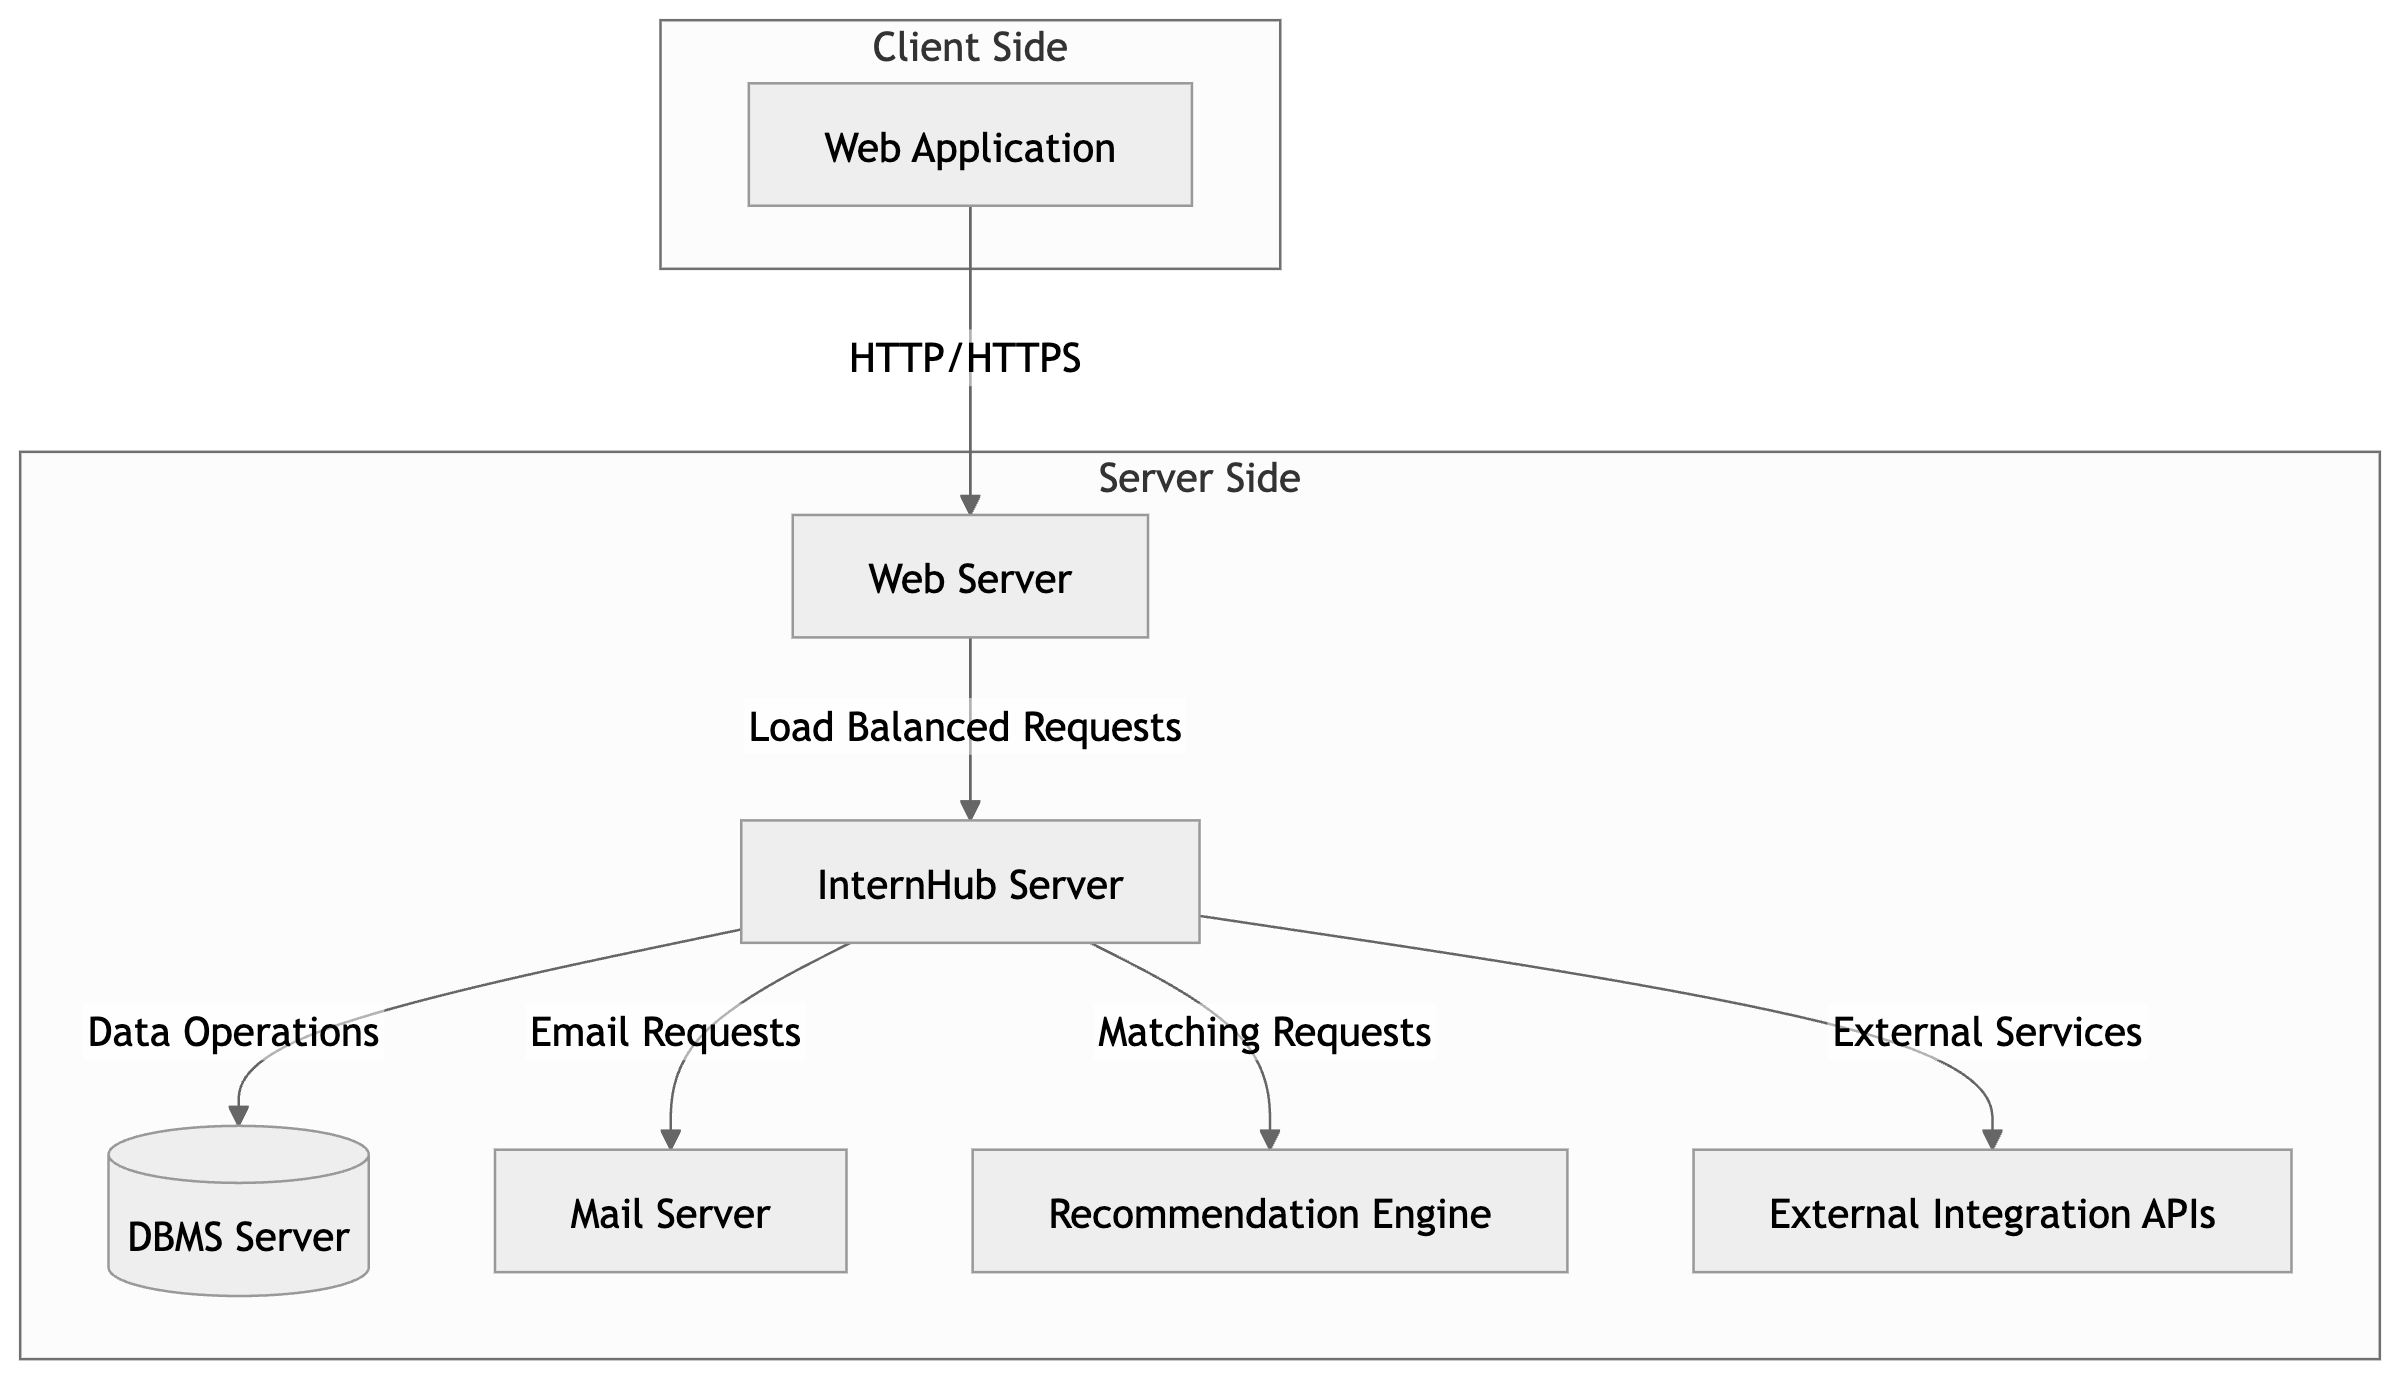
\includegraphics[width=0.82\linewidth]{JhaBhatiaSharma/imagesDD/CKB Overview.png}
        \caption{InternHub Overview}
        \label{fig:internHubOverview}%
    \end{center}
\end{figure}


\subsubsection{Client Side}
\begin{itemize}
    \item \textbf{Web Application:} The main user interface is the web application, which makes the platform accessible to all users—students, companies, and university administration. It makes it possible to do things like register, maintain profiles, post and apply for internships, handle complaints, and examine analytics.
\end{itemize}

\subsubsection{Server Side}
\begin{itemize}
    \item \textbf{Web Server:} Carries out user communications, taking in and processing their requests. For incoming requests, it offers load balancing and divides them among several S\&C Server replicas. To guarantee safe access, it also controls user sessions.
    \item \textbf{S\&C Server:} The center of the platform, which houses all of the interactions. It makes it easier for the database, Web Server, and external APIs to communicate with one another. To manage heavy traffic and guarantee availability, the S\&C Server is replicated over several computers.
    \item \textbf{DBMS Server:} Serves as the primary store for user, internship, application, feedback, and complaint data. It facilitates effective data retrieval and storage for all platform features.
    \item \textbf{Mail Server:} Manages email correspondence, including notifications for internships, changes, and user registration confirmation emails. By informing stakeholders, it improves the user experience.
    \item \textbf{Recommendation Engine API:} Uses advanced algorithms to recommend suitable internships to students based on their profiles and preferences, as well as potential candidates to companies.
    \item \textbf{Analytics Engine API:} Enables stakeholders to make data-driven decisions by offering insights and producing reports about internships, applications, and platform usage.
    \item \textbf{External Tools API:} Enables the safe storage and retrieval of internship-related files, including contracts and certificates, by facilitating integration with document management systems and other outside services.
\end{itemize}

\newpage

\section{Component View}
\label{subsec:component_view}

\subsection{High-Level Diagram}
\label{subsubsec:high_level_diagram}

\begin{figure}[H]
    \begin{center}
        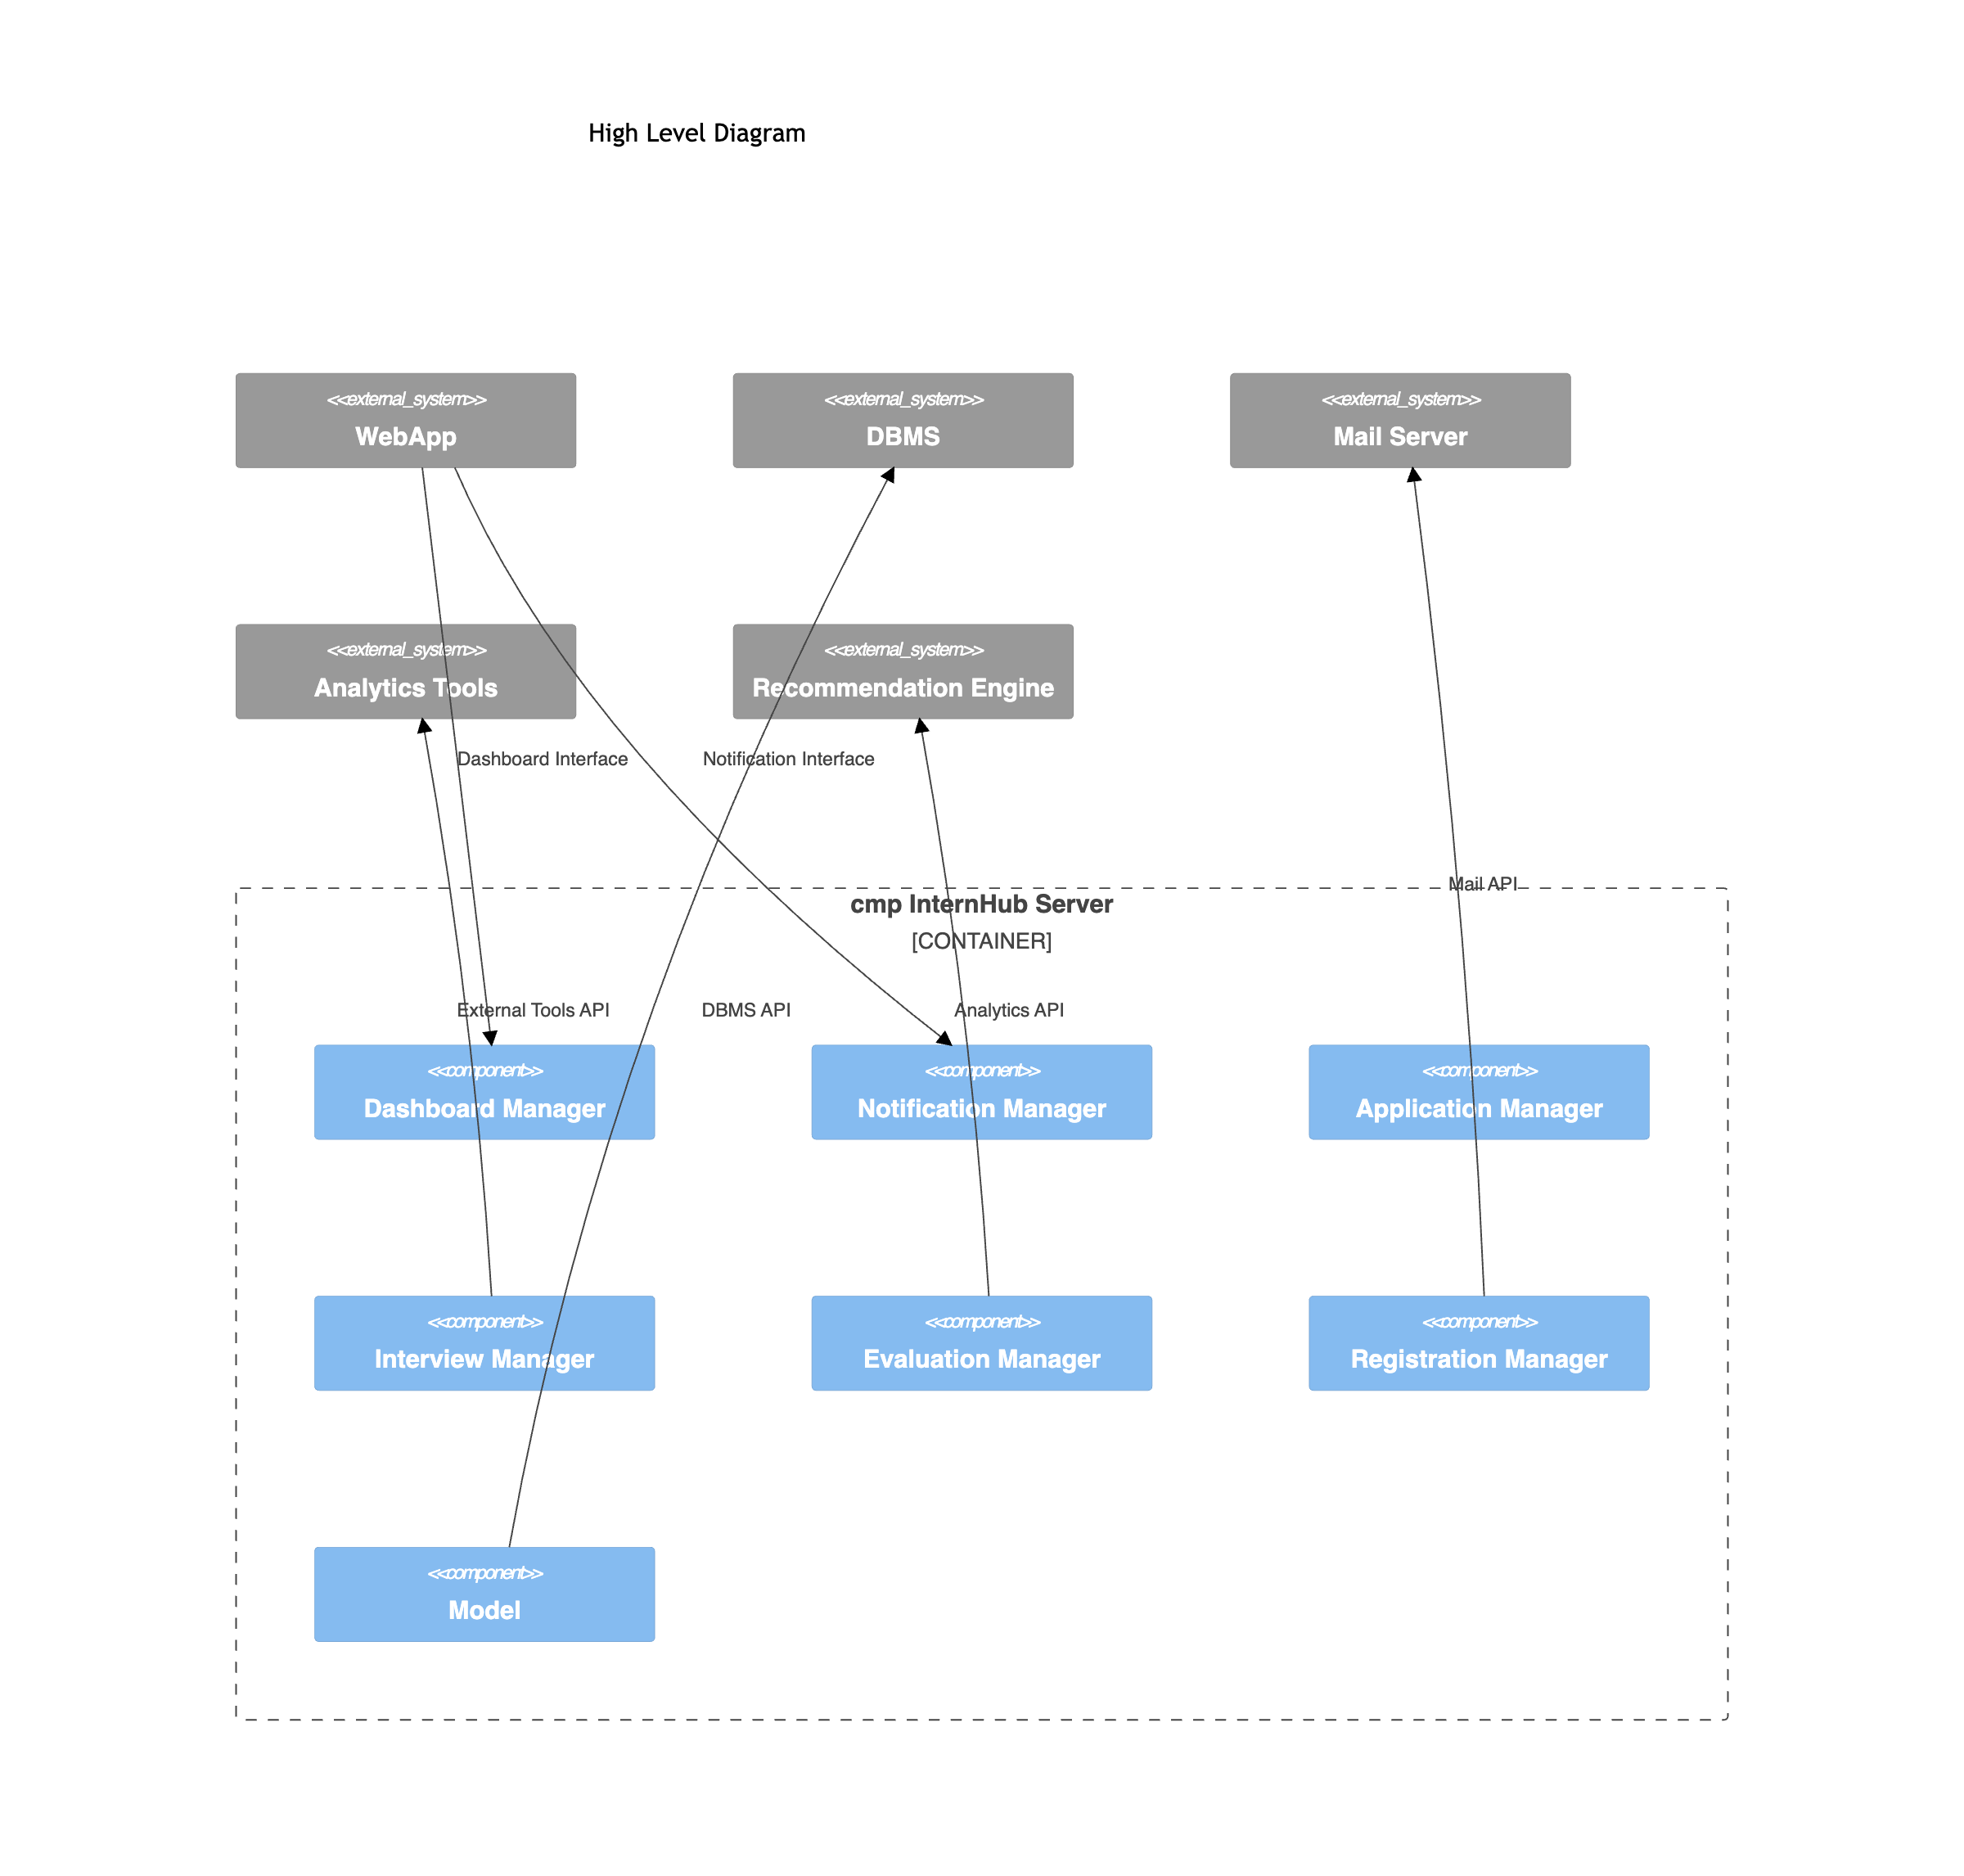
\includegraphics[width=0.82\linewidth]{JhaBhatiaSharma/imagesDD/High Level Diagram.png}
        \caption{High Level Diagram}
        \label{fig:highleveldiagram}%
    \end{center}
\end{figure}

The external components of S\&C are depicted in the high-level component diagram of S\&C above, along with their methods of communication with the S\&C server.

\begin{itemize}
    \item \textbf{WebApp:} Facilitates connectivity with the S\&C Server via the Dashboard Interface, the main channel for client-server communication, by acting as the external access point for users (students, businesses, and university administrators). Through the Notification Interface, the S\&C Server additionally notifies users of updates, reminders, and internship matches.
    \item \textbf{DBMS:} Serves as a storehouse for user profiles, applications, feedback, complaints, and internship posts. Through the DBMS API, which is controlled by the Model Component, it interacts with the S\&C Server.
    \item \textbf{Mail Server:} Manages email correspondence, including alerts for internships and confirmation emails sent after user registration. Through the Mail API, which is connected to the User Registration Manager component, the Mail Server can communicate with the S\&C Server.
    \item
    \textbf{Recommendation Engine:} Employs sophisticated algorithms to suggest internships to prospective employers and students. Through the Recommendation API, which is incorporated into the Matching Engine, it interacts with the S\&C Server.
    \item \textbf{Analytics Engine:} Provides data, analytics, and insights on platform activities, including system utilization, application success rates, and internship patterns. It uses the Analytics API to communicate with the S\&C Server.
    \item \textbf{Document Management System:} Makes it easier to store and retrieve internship-related paperwork securely, including contracts, certifications, and feedback reports. Through the Document Management API, which is incorporated into the File Manager component, it interfaces with the S\&C Server.

    \item \textbf{External System:}
    \begin{itemize}
    \item WebApp connects to the Dashboard Manager and Notification Manager using respective interfaces.
    \item DBMS connects to the Model using the DBMS API.
    \item Mail Server communicates with the Registration Manager through the Mail API.
    \item Recommendation Engine and Analytics Tools interact with the Notification Manager.
    \end{itemize}

    \item \textbf{InternHub Server:}
    The InternHub Server consists of core components like:
\begin{enumerate}
    \item Dashboard Manager
    \item Notification Manager
    \item Application Manager
    \item Registration Manager
    \item Evaluation Manager
    \item Interview Manager
    \item Model for centralized data access
\end{enumerate}
    
\end{itemize}

\subsection{Low-Level Diagram}
\label{subsubsec:low_level_diagram}

\begin{figure}[H]
    \begin{center}
        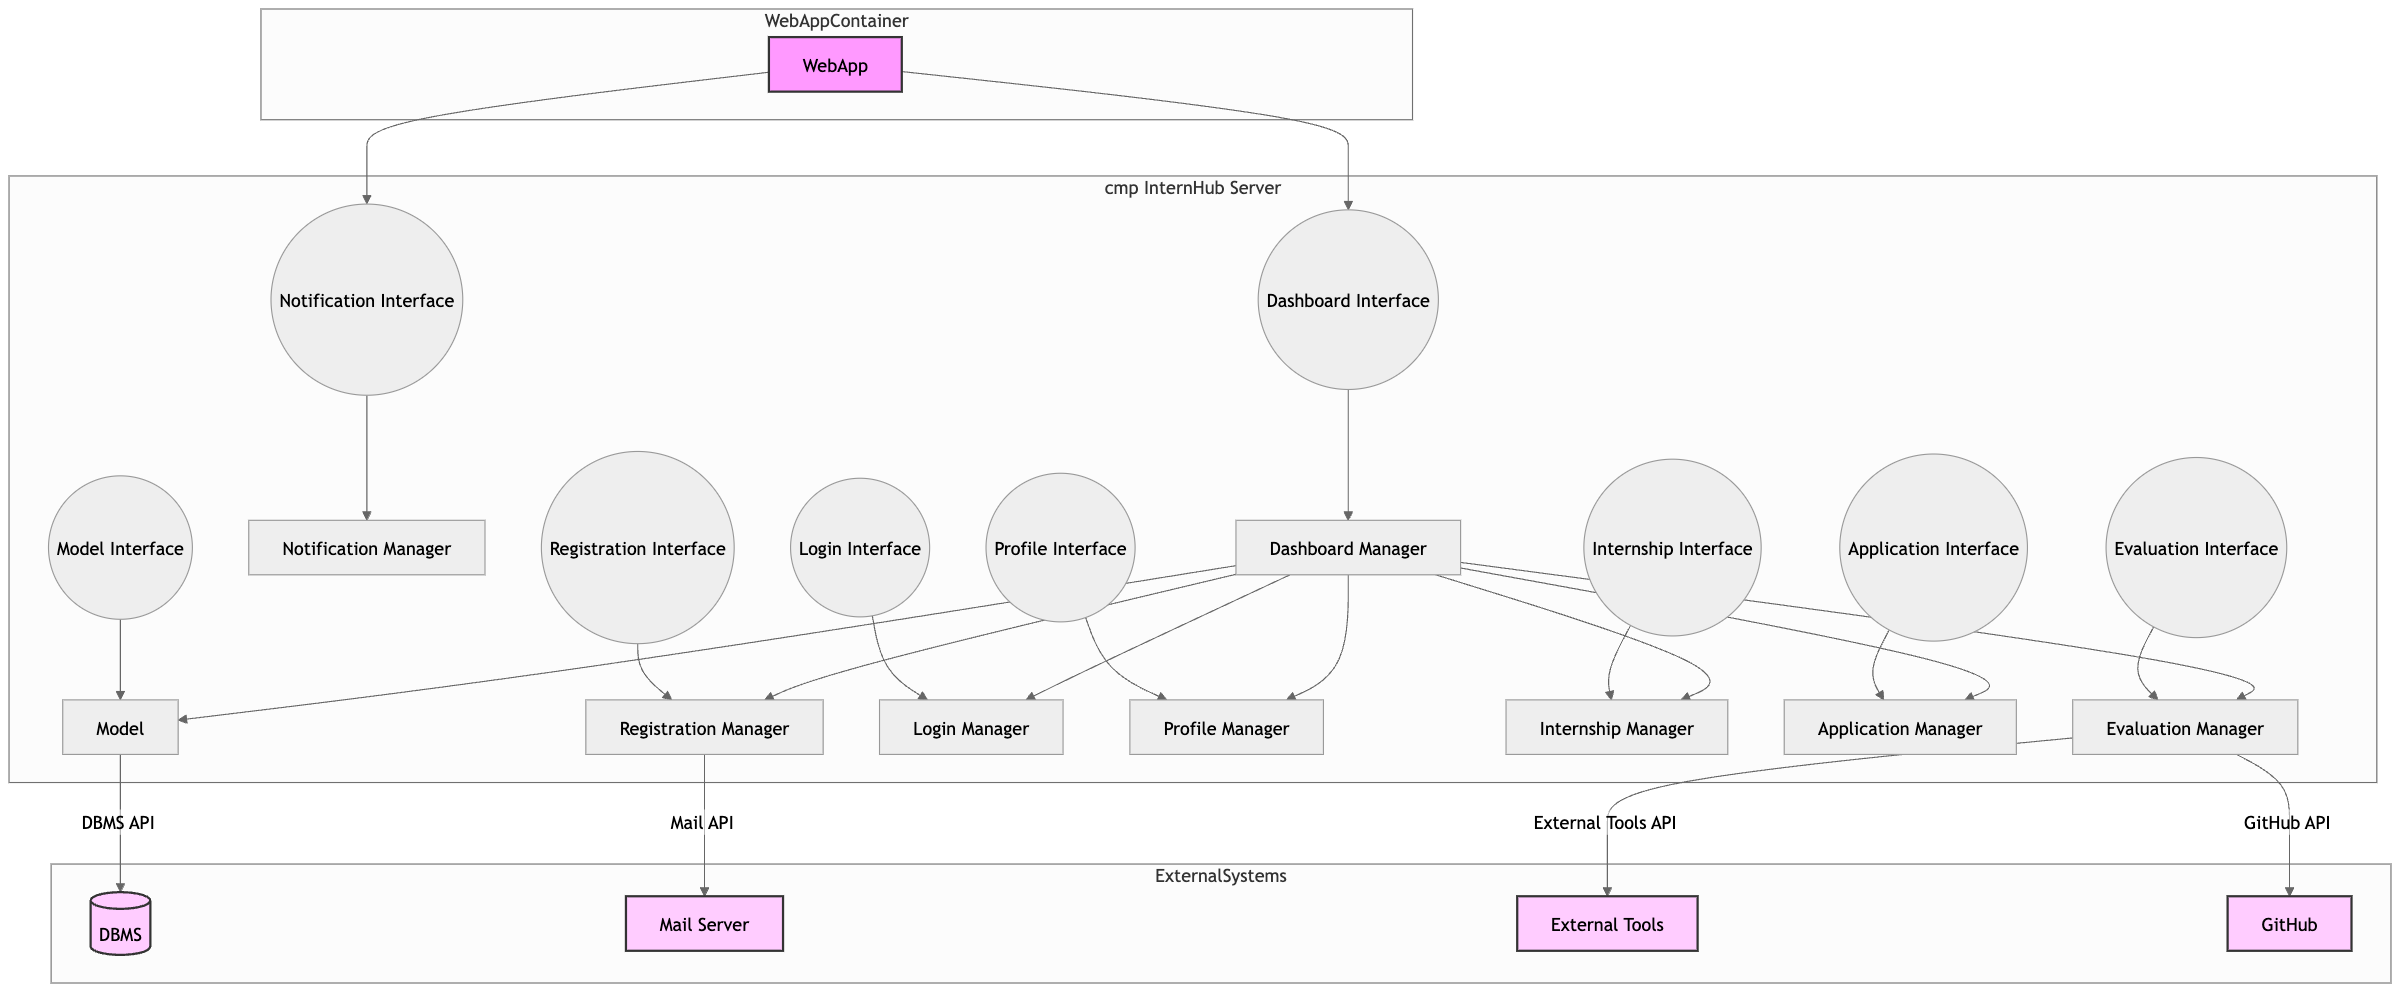
\includegraphics[width=0.82\linewidth]{JhaBhatiaSharma/imagesDD/LowLevelDiagram.png}
        \caption{Low Level Diagram}
        \label{fig:lowleveldiagram}%
    \end{center}
\end{figure}

The figure above represents the detailed architecture of the InternHub – Students \& Companies (S\&C) platform, showing the key components within the InternHub Server and their interactions.

\begin{itemize}
    \item \textbf{Dashboard Manager:} The essential element that plans out all user-platform communication. The Dashboard Manager routes user queries to the appropriate parts of InternHub, while the Dashboard Interface is how users engage with the platform. User activities including managing profiles, looking for internships, and receiving notifications all take place there.

    \item \textbf{Model Component:} Acts as a bridge interface to the DBMS Server and represents the data on the server. It guarantees that all components use the DBMS API to safely and effectively access data.

    \item \textbf{Registration Manager:} Manages the registration of new users, including companies, universities, and students. The Registration Manager handles requests made through the Registration Interface. It interacts with the Model Component to add new user information to the database and with the Mail Server via the Mail API to deliver confirmation emails.

    \item \textbf{Login Manager:} Oversees the registered users' login procedure. The Login Manager handles user login requests sent through the Login Interface. It collects user data from the Model Component and verifies credentials.

    \item \textbf{Profile Manager:} Enables users to search for and browse other users' profiles in addition to managing their own. In order to retrieve or change profile data, the Profile Manager interacts with the Model Component via the Profile Interface.

    \item \textbf{Internship Manager:} Oversees all internship-related activities, such as job advertisements, applications, and status reports.
    \item \textbf{Application Manager:} Manages internship applications, including submission, alerts, and status monitoring. It interacts with the Model Component to retrieve and update data and handles requests through the Application Interface.

    \item \textbf{Evaluation Manager:} Handles the evaluation of students' success during internships.
    \item \textbf{Notification Manager:} In charge of managing every notification that users get. It handles requests through the Notification Interface, including alerting users to platform events, application updates, and internship postings. It interacts with other managers for event triggers and the Model Component for storing notification data.

\end{itemize}

\subsection{Evaluation Manager}
\label{subsubsec:evaluation_manager}
\begin{figure}[H]
    \begin{center}
        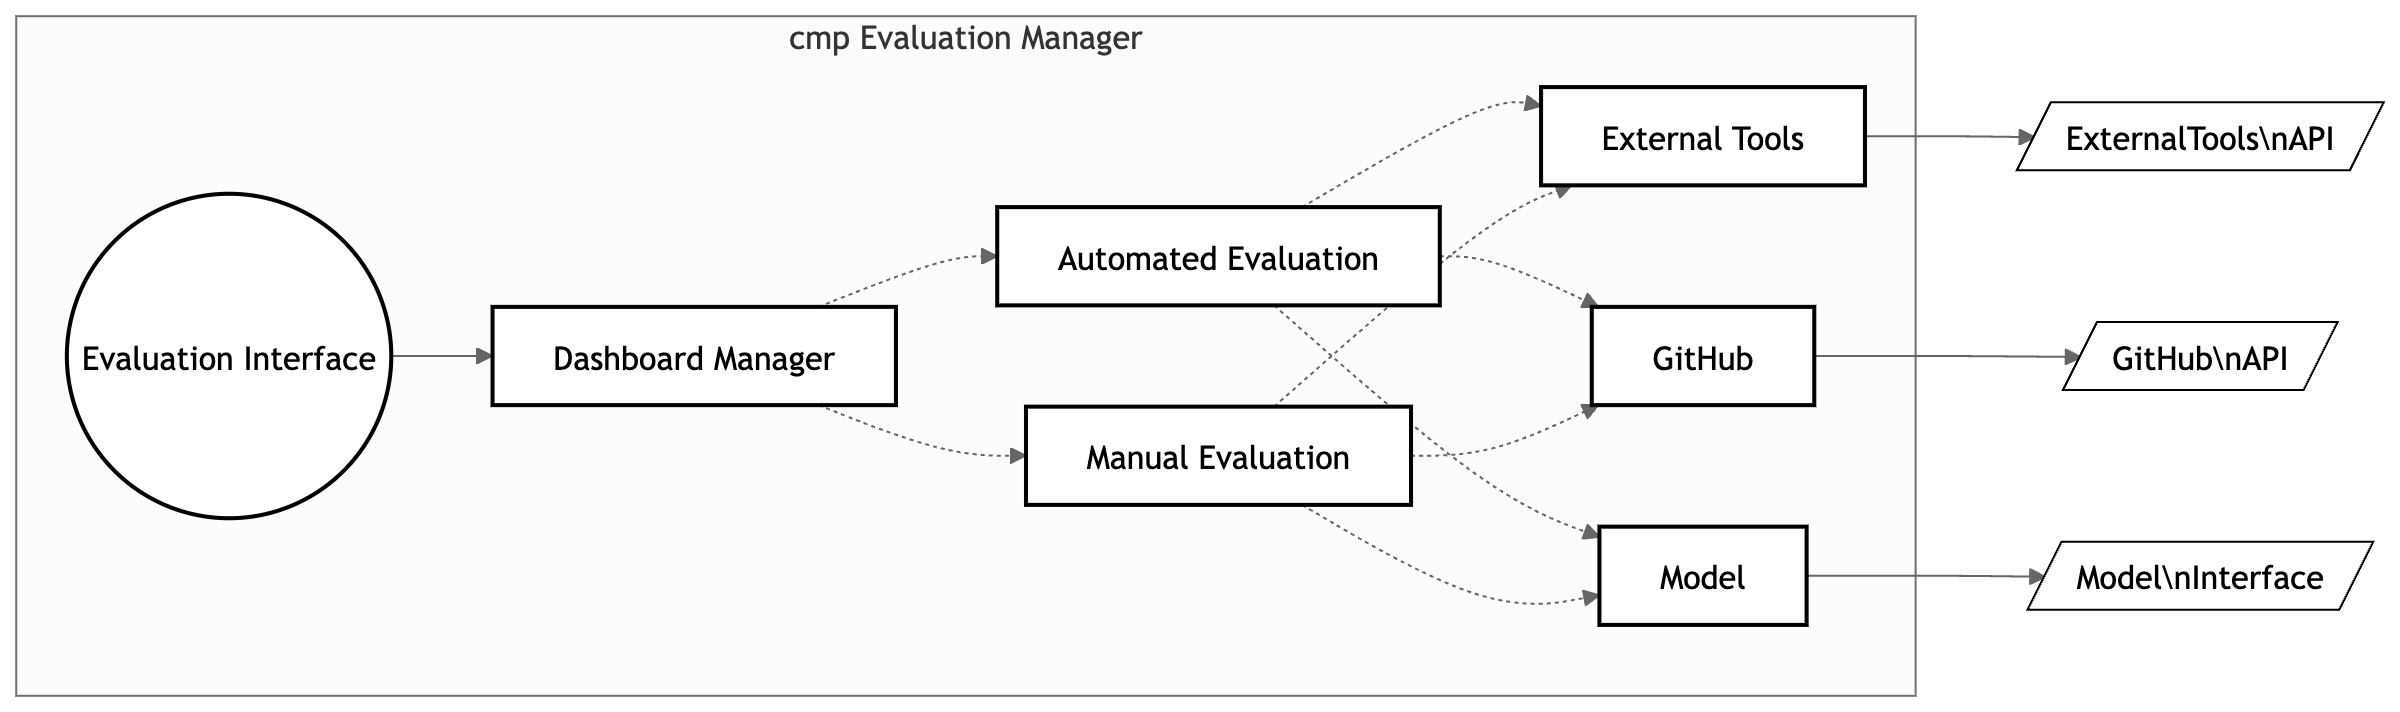
\includegraphics[width=0.82\linewidth]{JhaBhatiaSharma/imagesDD/EvaluationManager.png}
        \caption{Evaluation Manager}
        \label{fig:evaluationmanager}%
    \end{center}
\end{figure}
The InternHub – Students \& Companies (S\&C) platform's Evaluation Manager is designed to evaluate and oversee students' performance reviews during internships. To manage various evaluation techniques, it is divided into two sub-components: Automated Evaluation and Manual Evaluation.

\subsubsection{Automated Evaluation Component}
The Automated Evaluation component is utilized by the InternHub system to automatically assess a student’s performance or task completion during their internship. The workflow is as follows:
\begin{enumerate}
    \item Through the Evaluation Interface, the system notifies the Automated Evaluation Component when an internship milestone or work submission takes place.
    \item Through the External Tools API, the Automated Evaluation component forwards the submitted work to outside tools for evaluation, testing, or scoring (e.g., project testing or task completion verification).
    \item The Automated Evaluation component uses the Model Interface to communicate with the Model Component after receiving the evaluation results from the external tools.
    \item In turn, the Model Component uses the DBMS API to update the student's score in the database, guaranteeing that the evaluation results are appropriately recorded in the appropriate database area.
\end{enumerate}

\subsubsection{Manual Evaluation Component}
The Manual Evaluation component allows companies or university administrators to manually assess a student’s performance during their internship. The process is as follows:
\begin{enumerate}
    \item The evaluator (company or administrator) initiates a request via the WebApp, which connects to the Dashboard Interface.
    \item Through the Evaluation Interface, the request is sent to the Manual Evaluation Component.
    \item The GitHub API or other integrated technologies are used by the Manual Evaluation component to retrieve the student's submitted work or internship data.
    \item The Manual Evaluation component uses the Model Interface to provide the updated results to the Model Component following the evaluator's manual analysis and scoring.
    \item The Model Component ensures that the outcomes of the manual evaluation are accurately documented by updating the scores or evaluations in the database using the DBMS API.
\end{enumerate}

\subsection{Dashboard Manager}
\label{subsubsec:dashboard_manager}

\begin{figure}[H]
    \begin{center}
        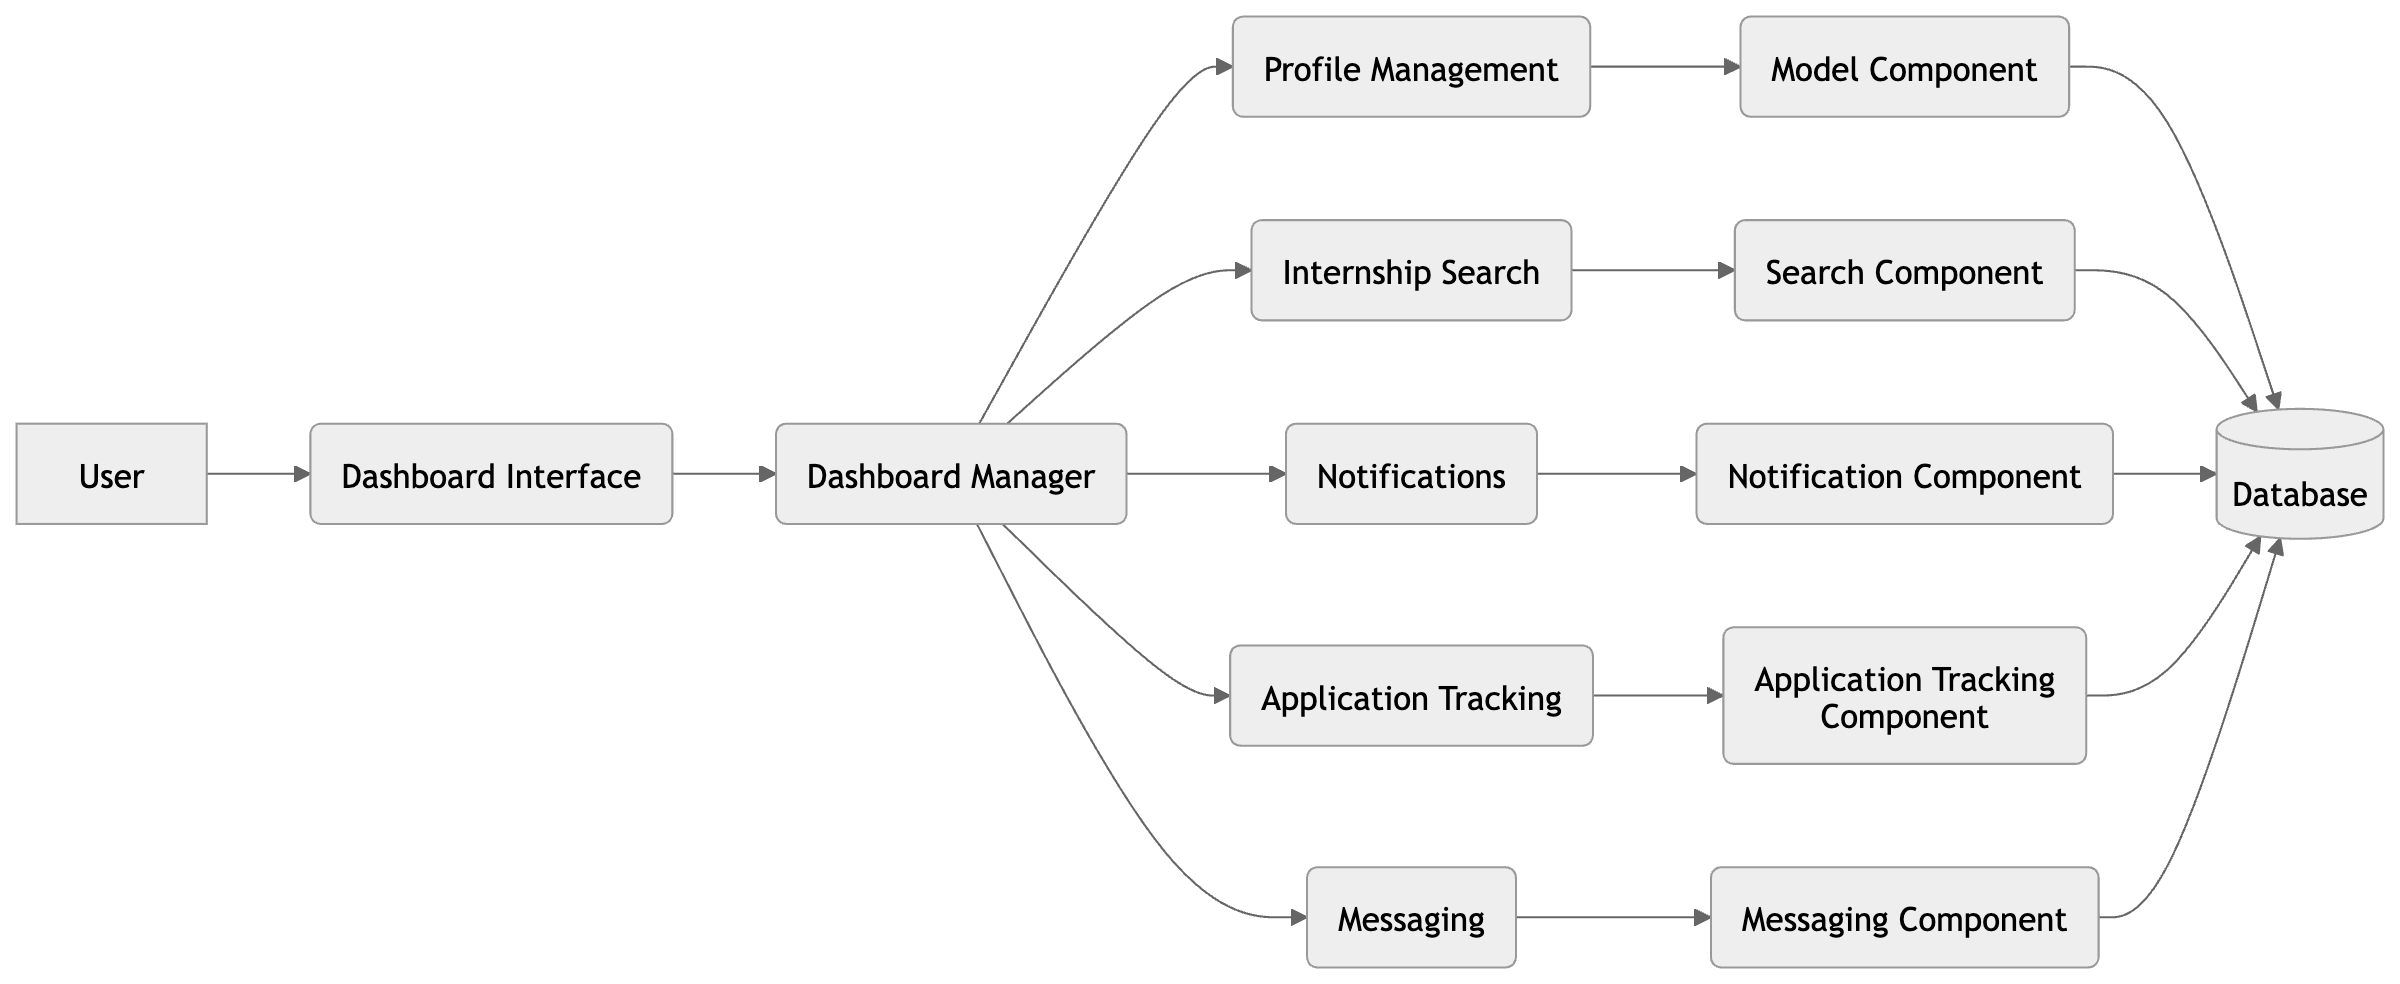
\includegraphics[width=0.82\linewidth]{JhaBhatiaSharma/imagesDD/DashboardManager.png}
        \caption{Dashboard Manager}
        \label{fig:dashboardmanager}%
    \end{center}
\end{figure}

The Dashboard Manager is a pivotal component in the InternHub – Students \& Companies (S\&C) platform, managing user interactions and orchestrating communication between various subsystems. The following outlines its subcomponents and their interactions:

\paragraph{Profile Management}
Users can manage and update their profiles, which include contact details, preferences, and resumes.
\begin{itemize}
    \item In order to retrieve or change user data, the Model Component communicates with the Database and receives requests pertaining to profile management.
\end{itemize}

\paragraph{Internship Search}
Allows users to search and filter internships based on location, preferences, and skills.
\begin{itemize}
    \item These requests are handled by the Search Component, which queries the database and provides users with pertinent results through the Dashboard Interface.
\end{itemize}

\paragraph{Notifications}
Oversees the distribution of user notifications, including critical system messages, profile recommendations, and updates to internship applications.
\begin{itemize}
    \item Interacts with the Notification Component, which provides notification logs and status updates to the database.
\end{itemize}

\paragraph{Application Tracking}
Allows users to keep track of the acceptance, rejection, and company updates on their internship applications.
\begin{itemize}
    \itemIn order to retrieve and present current application statuses, the Application Tracking Component communicates with the database.
\end{itemize}

\paragraph{Messaging}
Facilitates direct communication between administration, businesses, and students to address questions or discuss internships.
\begin{itemize}
    \item Communicates with the Messaging Component, which guarantees that every conversation is recorded and safely kept in the database.
\end{itemize}

\subsection{Profile Manager}
\label{subsubsec:profile_manager}

\begin{figure}[H]
    \begin{center}
        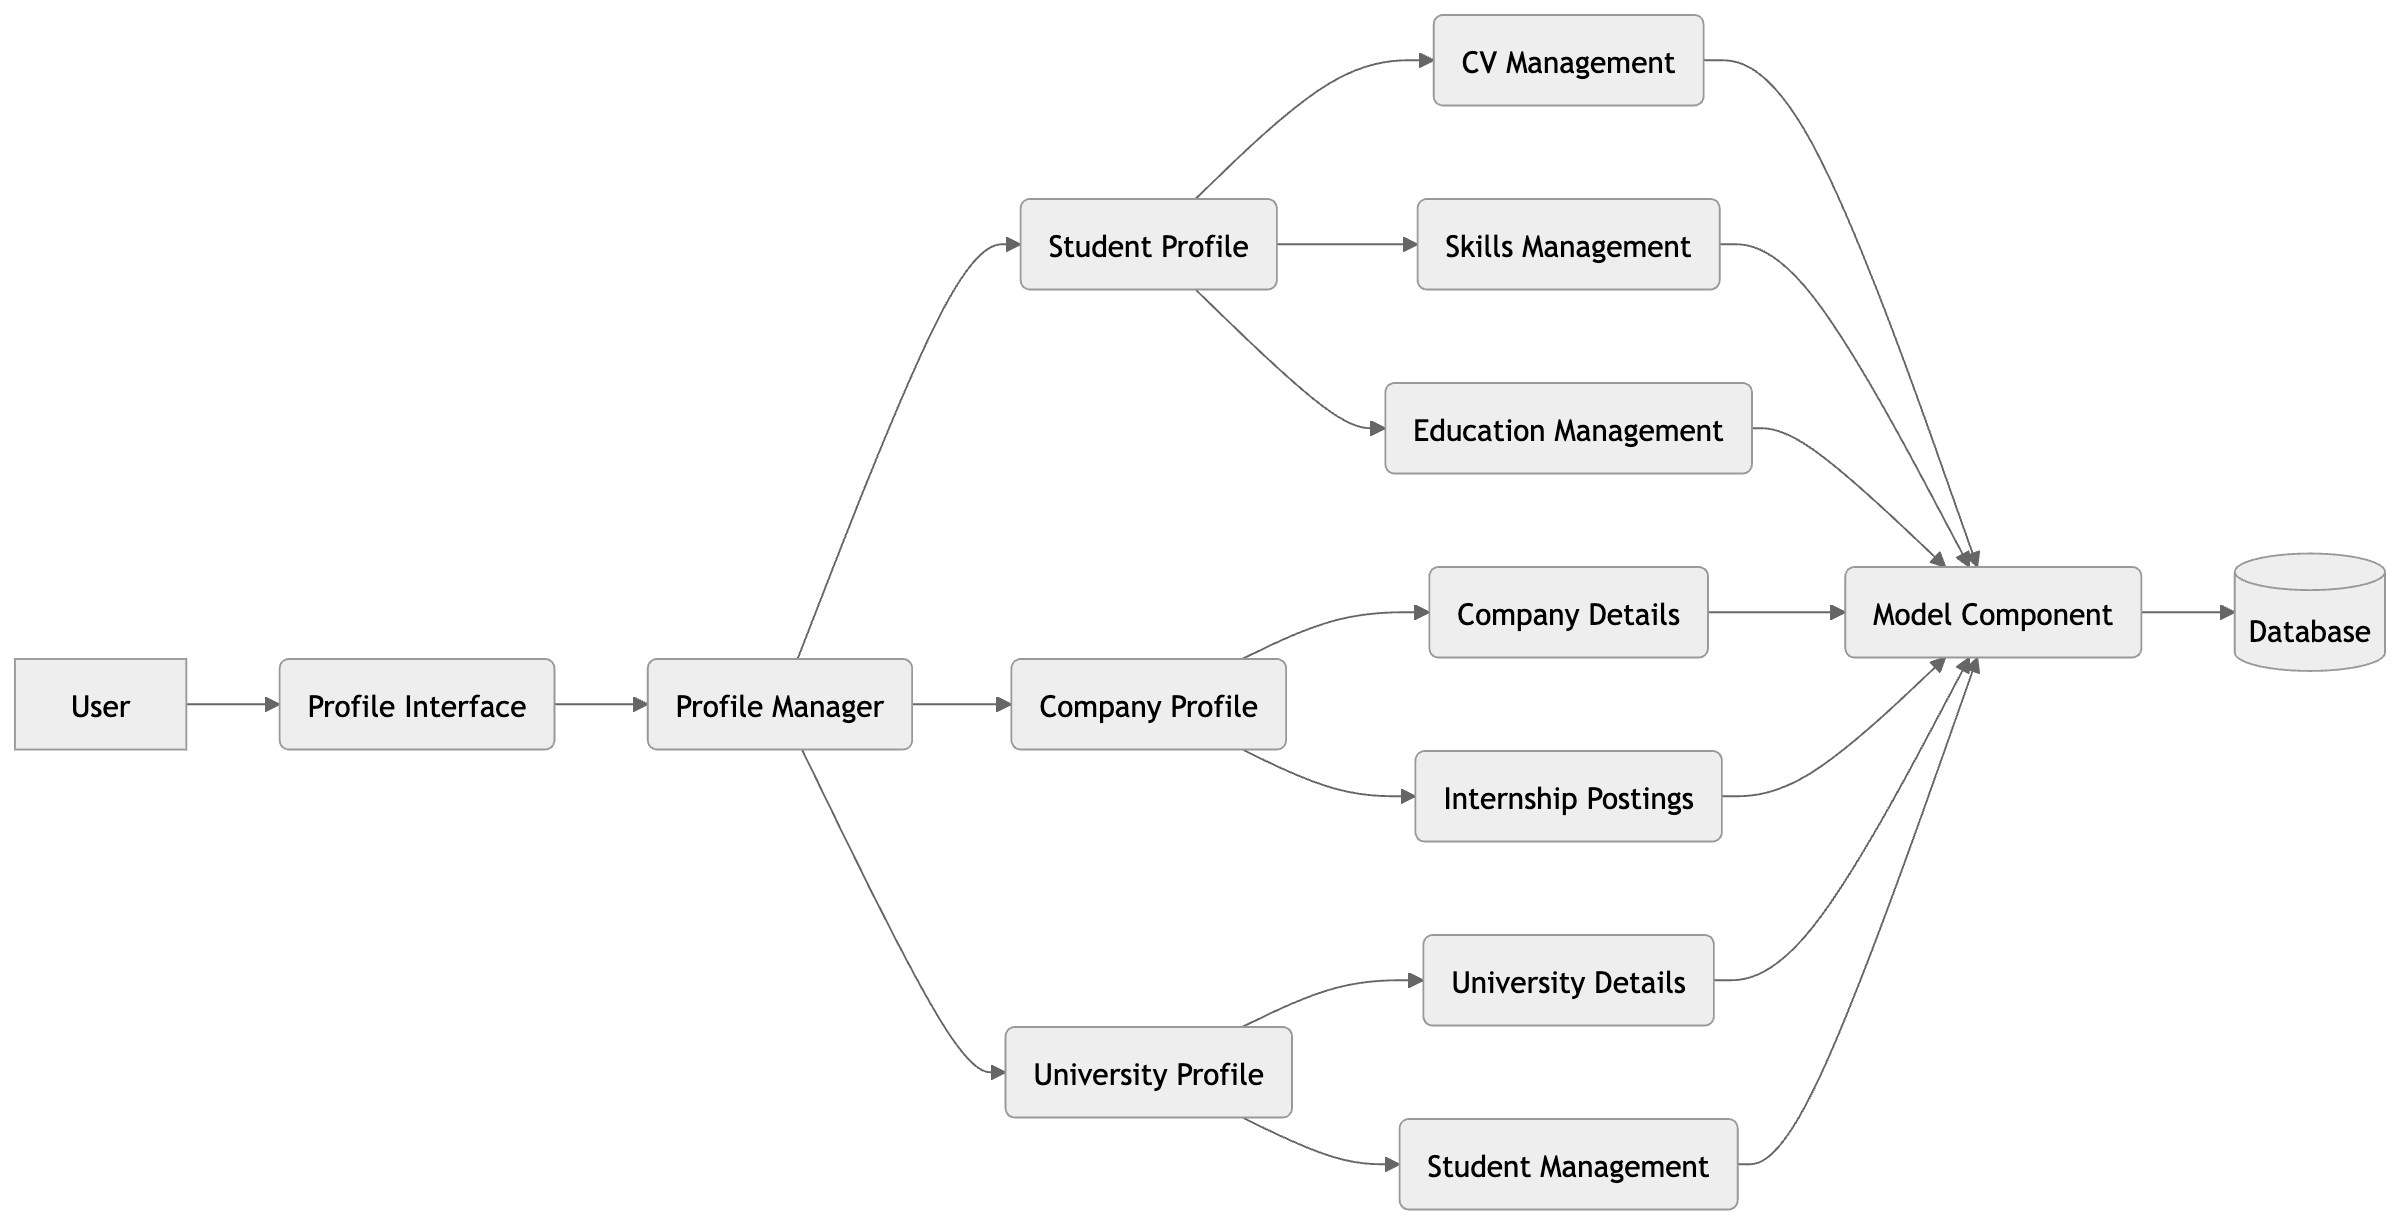
\includegraphics[width=0.82\linewidth]{JhaBhatiaSharma/imagesDD/ProfileManager.png}
        \caption{Profile Manager}
        \label{fig:profilemanager}%
    \end{center}
\end{figure}

The InternHub – Students \& Companies (S\&C) platform's Profile Manager is a key feature that helps institutions, businesses, and students manage and streamline profile-related tasks. To efficiently handle user profile data, the component ensures seamless communication between the Model Component and the database. These are the main subcomponents and their responsibilities:

\paragraph{Student Profile}
Manages student-specific details, including academic achievements, skills, and internship preferences.
\begin{itemize}
    \item \textbf{CV Management:} Handles the creation, modification, and storage of student CVs.
    \item \textbf{Skills Management:} Allows students to add, update, or remove skills based on their expertise.
    \item \textbf{Education Management:} Manages educational history and academic records.
\end{itemize}

\paragraph{Company Profile}
Responsible for maintaining company-related data, such as organizational details, internship postings, and company preferences.
\begin{itemize}
    \item \textbf{Company Details:} Stores and updates company information, such as name, size, industry, and contact details.
    \item \textbf{Internship Postings:} Enables companies to create, modify, and manage internship listings.
\end{itemize}

\paragraph{University Profile}
Oversees university-specific information and ensures administrators have tools to manage student profiles and internships.
\begin{itemize}
    \item \textbf{University Details:} Handles institutional information, including department details and associated staff.
    \item \textbf{Student Management:} Allows universities to monitor and manage student data and progress.
\end{itemize}

\subsection{Internship Manager}
\label{subsec:internship_manager}
\begin{figure}[H]
    \begin{center}
        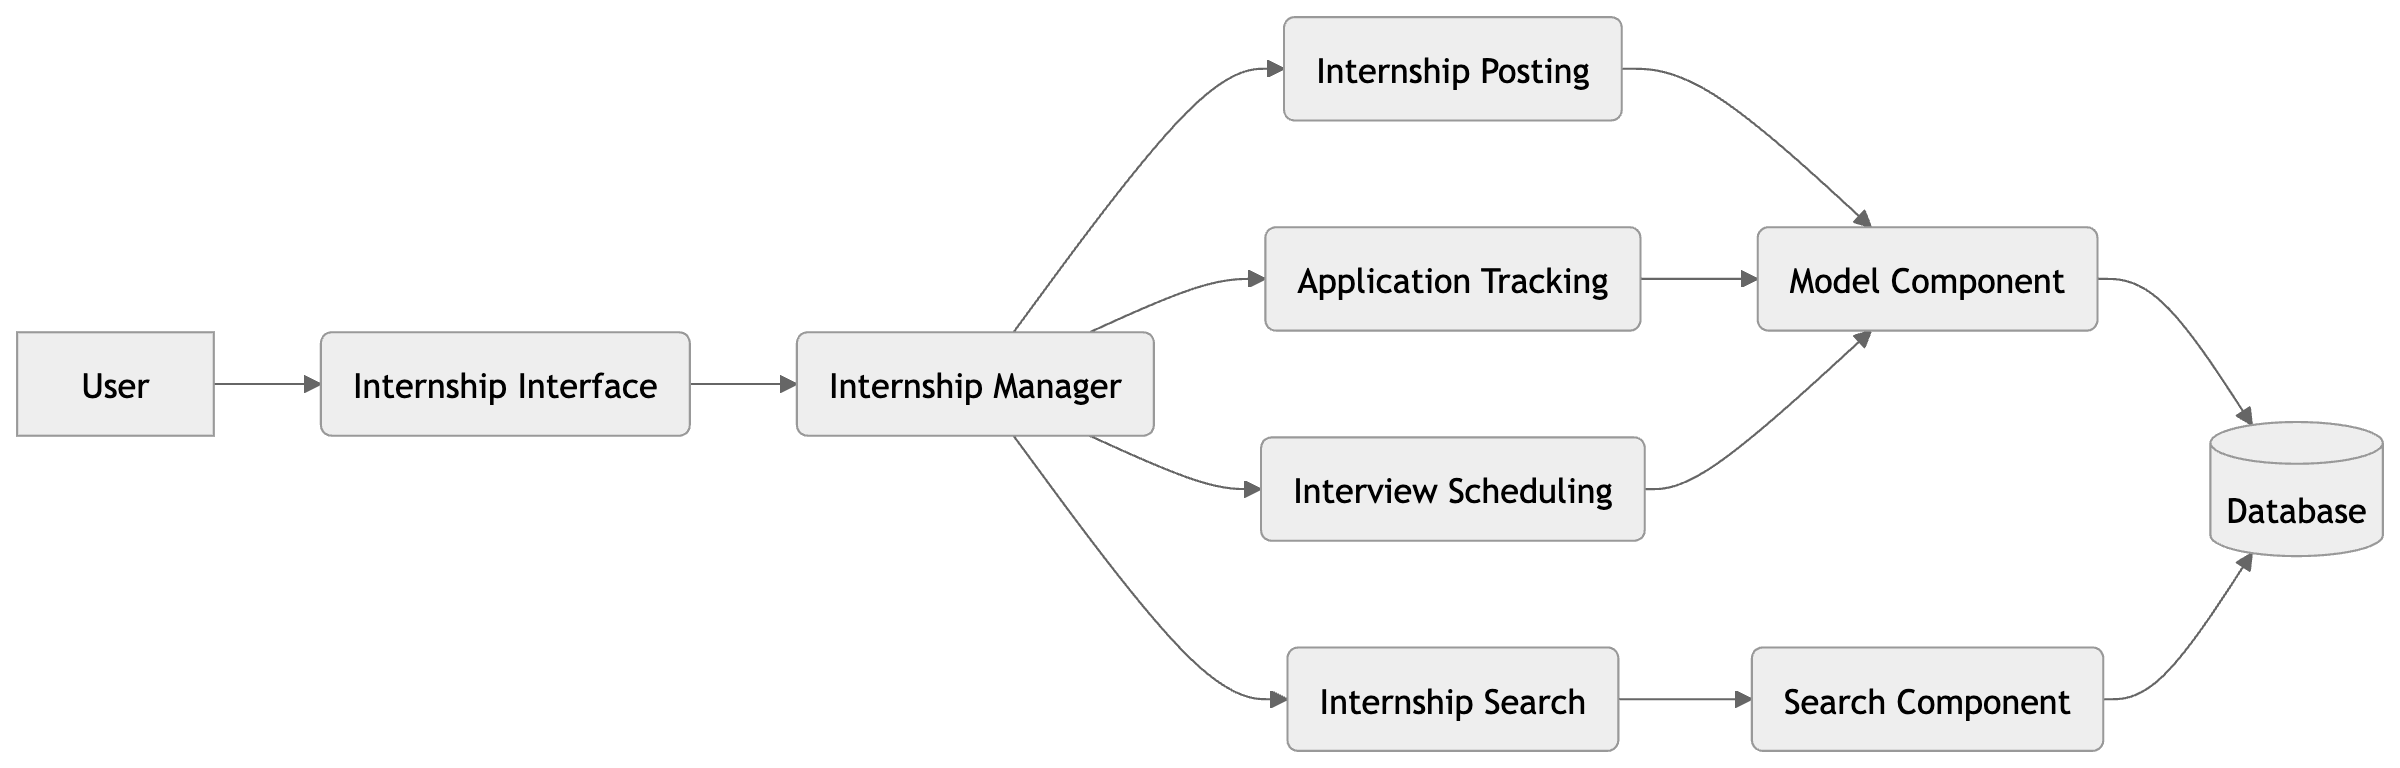
\includegraphics[width=0.82\linewidth]{JhaBhatiaSharma/imagesDD/InternshipManager.png}
        \caption{Internship Manager}
        \label{fig:internshipmanager}%
    \end{center}
\end{figure}

Managing the internship lifecycle is the primary responsibility of the InternHub – Students \& Companies (S\&C) platform's Internship Manager. It facilitates effective handling of internship-related features by managing user interactions with the platform. Below is a summary of its constituents and interrelations:

\paragraph{Internship Posting}
\begin{itemize}
    \item Allows companies to create, update, and manage internship opportunities.
    \item Interacts with the Model Component to store and retrieve data from the Database.
    \item Ensures all postings are accessible to students via the Internship Search feature.
\end{itemize}

\paragraph{Application Tracking}
\begin{itemize}
    \item Enables students and companies to monitor the status of internship applications in real-time.
    \item Communicates with the Model Component to update and retrieve application details from the Database.
    \item Provides notifications to users regarding application progress or results.
\end{itemize}

\paragraph{Interview Scheduling}
\begin{itemize}
    \item Handles the scheduling of interviews between students and companies as part of the internship process.
    \item Retrieves and updates scheduling data in the Database through the Model Component.
\end{itemize}

\paragraph{Internship Search}
\begin{itemize}
    \item Helps students search for internships based on criteria such as location, skills, or duration.
    \item Uses the Search Component to query the Database and fetch matching results.
    \item Provides personalized recommendations based on student profiles and preferences.
\end{itemize}

\subsection{Application Manager}
\label{subsec:application_manager}
\begin{figure}[H]
    \begin{center}
        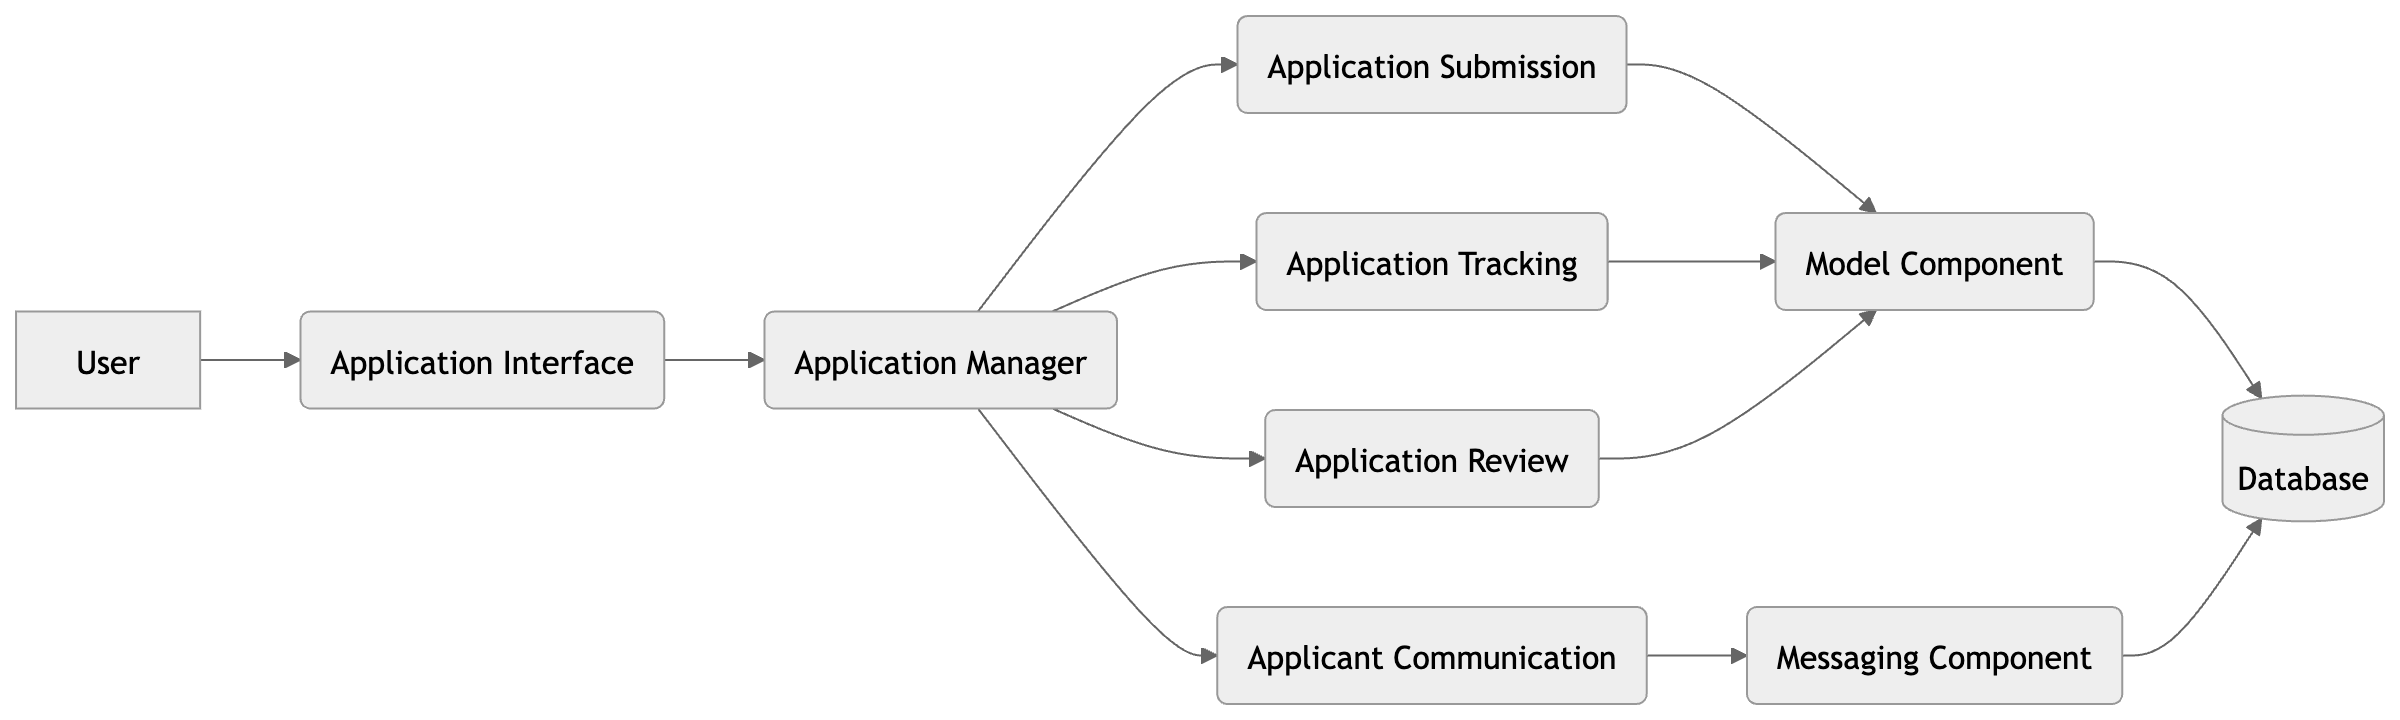
\includegraphics[width=0.82\linewidth]{JhaBhatiaSharma/imagesDD/ApplicationManager.png}
        \caption{Application Manager}
        \label{fig:applicationmanager}%
    \end{center}
\end{figure}

The Application Manager is responsible for handling all operations related to internship applications, ensuring seamless interaction between students, companies, and the platform.

\paragraph{Application Submission}
\begin{itemize}
    \item Manages the submission of internship applications by students.
    \item Interacts with the Model Component to store the application data in the Database.
\end{itemize}

\paragraph{Application Tracking}
\begin{itemize}
    \item Allows students and companies to monitor the status of submitted applications.
    \item Communicates with the Model Component to retrieve and update application status in the Database.
\end{itemize}

\paragraph{Application Review}
\begin{itemize}
    \item Enables companies to review applications submitted by students.
    \item Retrieves application details from the Model Component and updates the status post-review in the Database.
\end{itemize}

\paragraph{Applicant Communication}
\begin{itemize}
    \item Facilitates direct communication between applicants and companies regarding applications.
    \item Utilizes the Messaging Component to send and receive messages, with all interactions logged in the Database.
\end{itemize}

\section{Deployment View}
\label{sec:deployment_view}

\begin{figure}[H]
    \begin{center}
        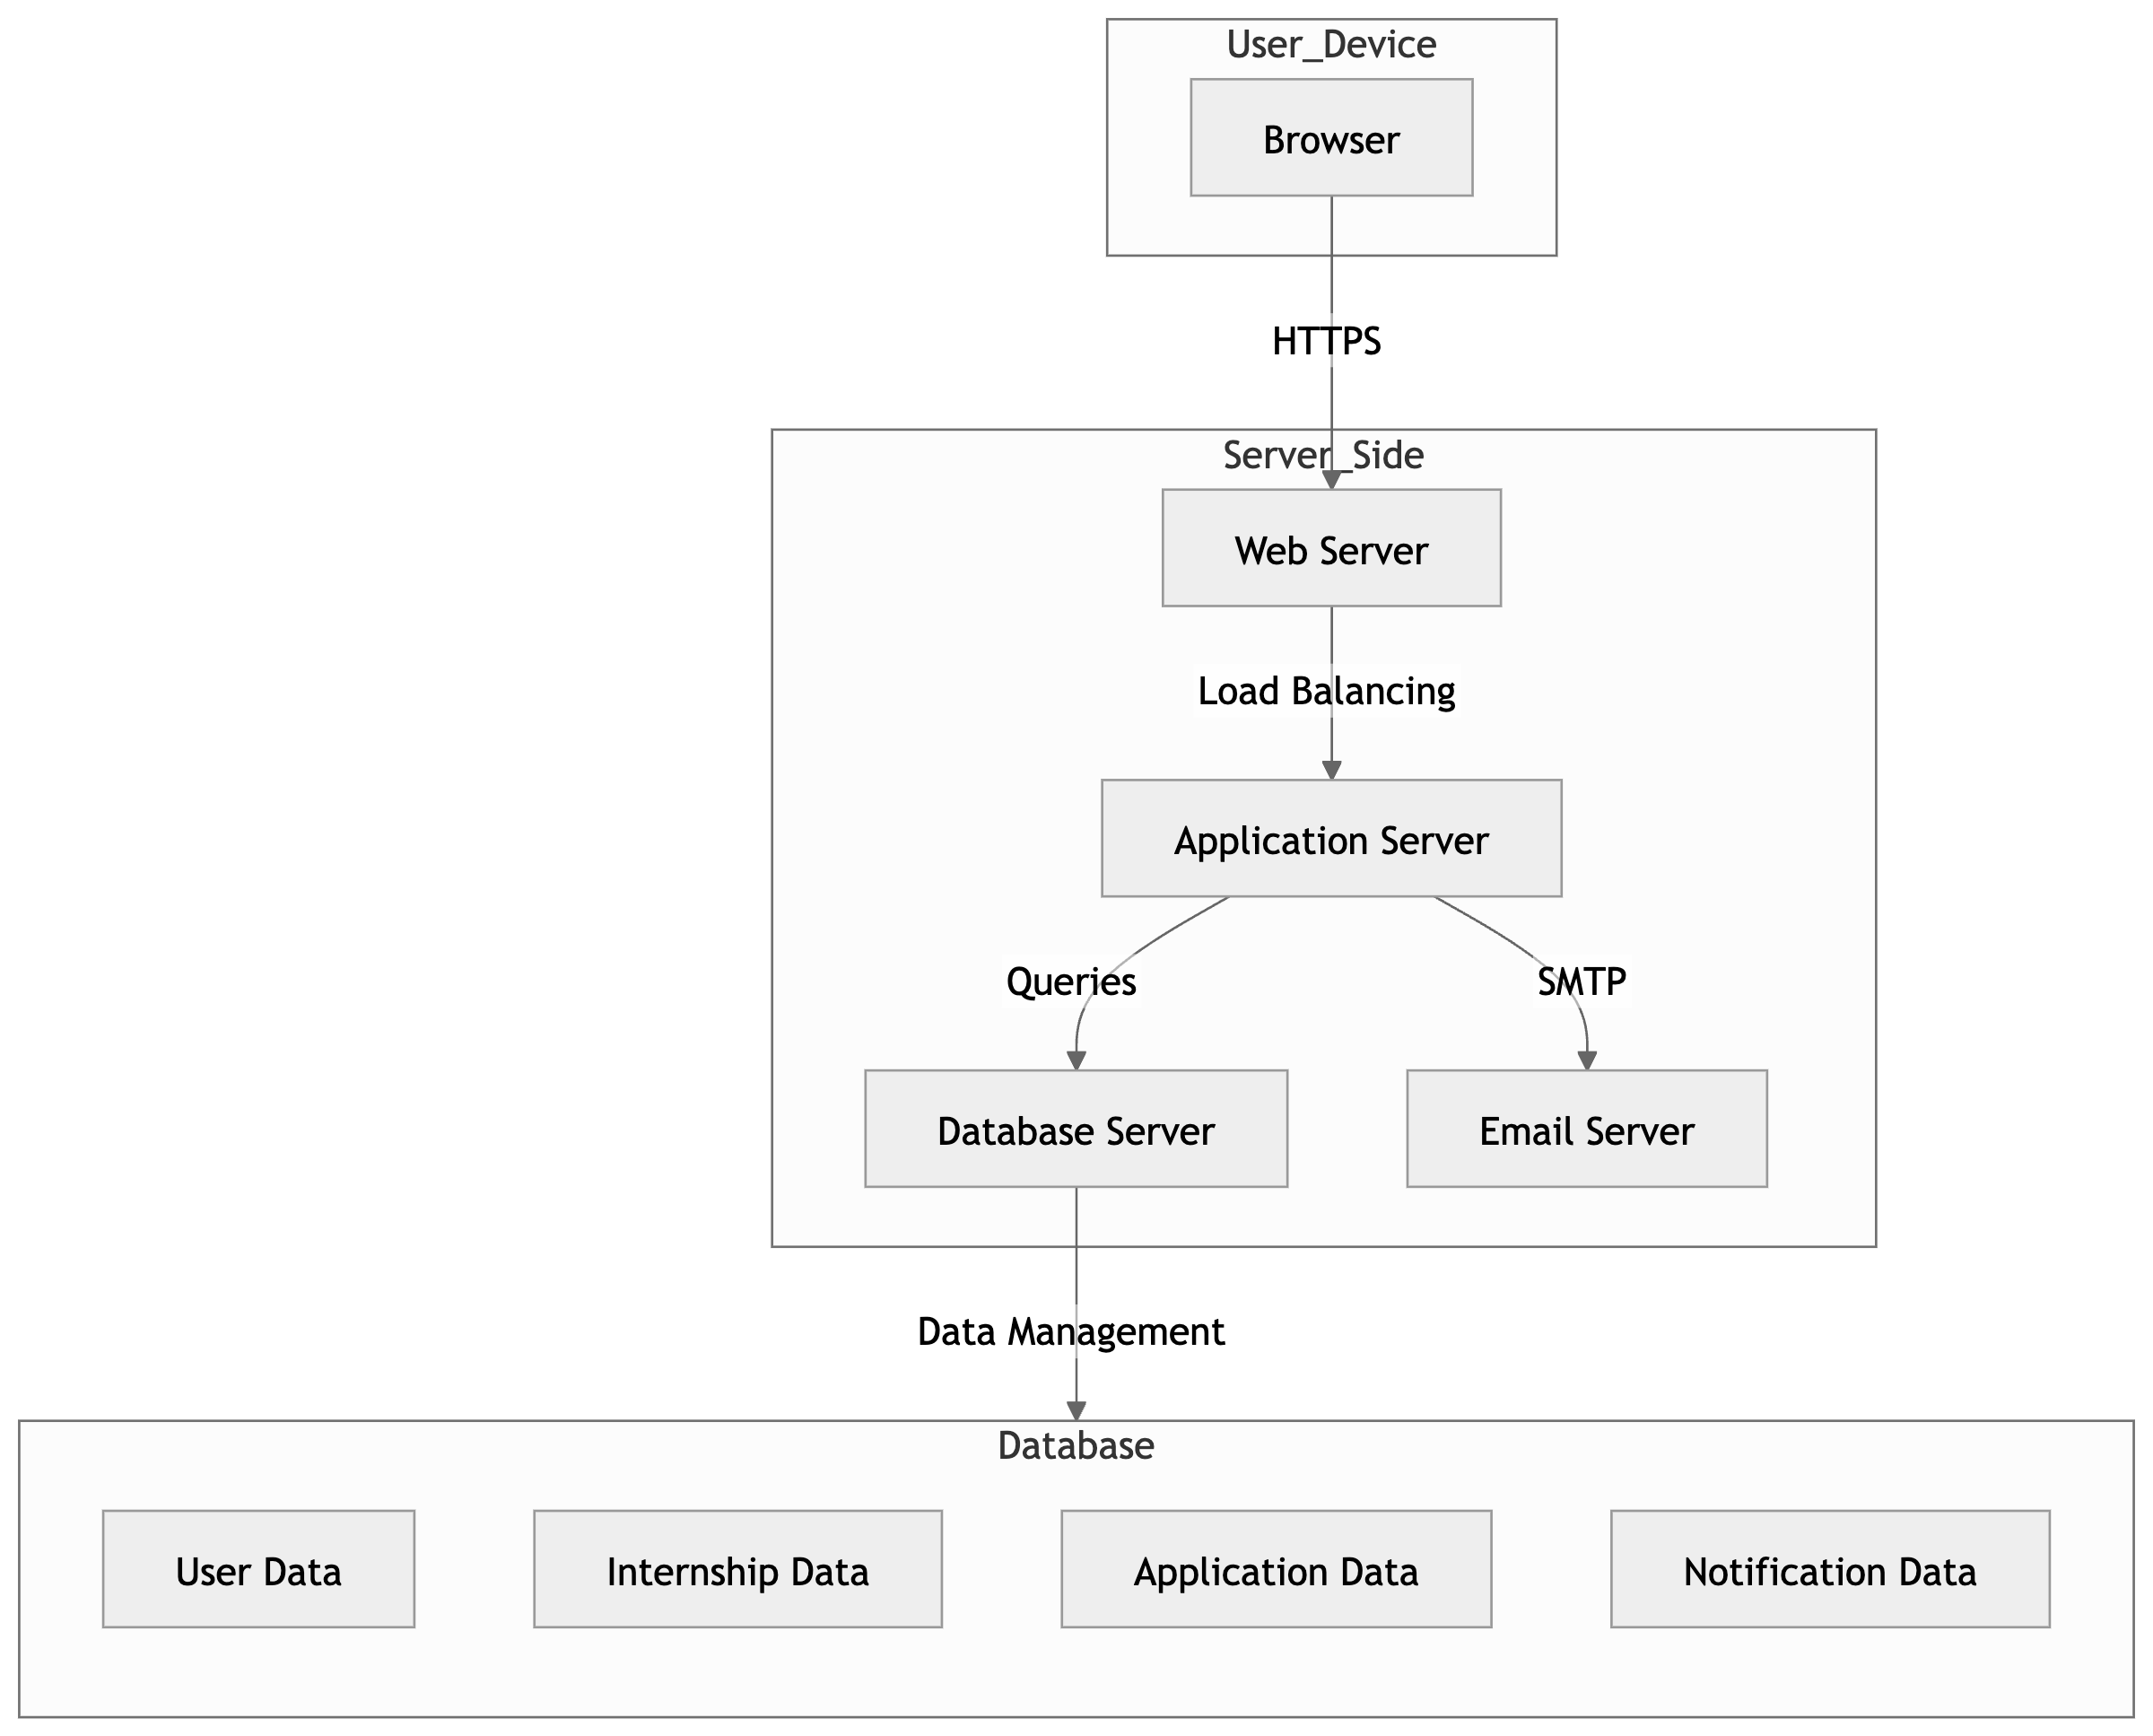
\includegraphics[width=0.82\linewidth]{JhaBhatiaSharma/imagesDD/DeploymentView.png}
        \caption{Deployment View}
        \label{fig:deploymentview}%
    \end{center}
\end{figure}
The platform's deployment architecture is composed of the following layers:

\paragraph{Client Side}
\begin{itemize}
    \item User devices, which are mostly accessed through web browsers, make up the client side. These devices stand in for platform users, which include companies, educational institutions, and students.
    \item Users engage with platform services such as applications, notifications, internship posts, profile management, registration, and login using their browsers.
    \item HTTPS ensures data privacy and protection by securing communication between the user and the platform.
\end{itemize}

\paragraph{Server Side}
\begin{itemize}
    \item \textbf{Web Server:} serves as the gateway for all requests from clients. By allocating incoming requests to several application server replicas, it performs load balancing, guarantees secure HTTPS connections, and controls the delivery of static content (HTML, CSS, and JavaScript).
    \item \textbf{Application Server:} acts as the main backend, coordinating with other parts and processing business logic. Notification delivery, internship management, and user management are all handled by it. For data storage and retrieval, it interfaces with the DBMS Server; for automated communication, it integrates with the Email Server.
    \item \textbf{DBMS Server:} keeps application, user, and internship-related data. Notifications are recorded, and effective data updates, retrieval, and storage are guaranteed.
    \item \textbf{Email Server:} uses the SMTP protocol to handle outward messages, including application updates and registration confirmations.
\end{itemize}

\section{Runtime View}
\label{sec:runtime_view}

\subsection{Sign-Up Process}
\label{subsec:signup_process}
\begin{figure}[H]
    \begin{center}
        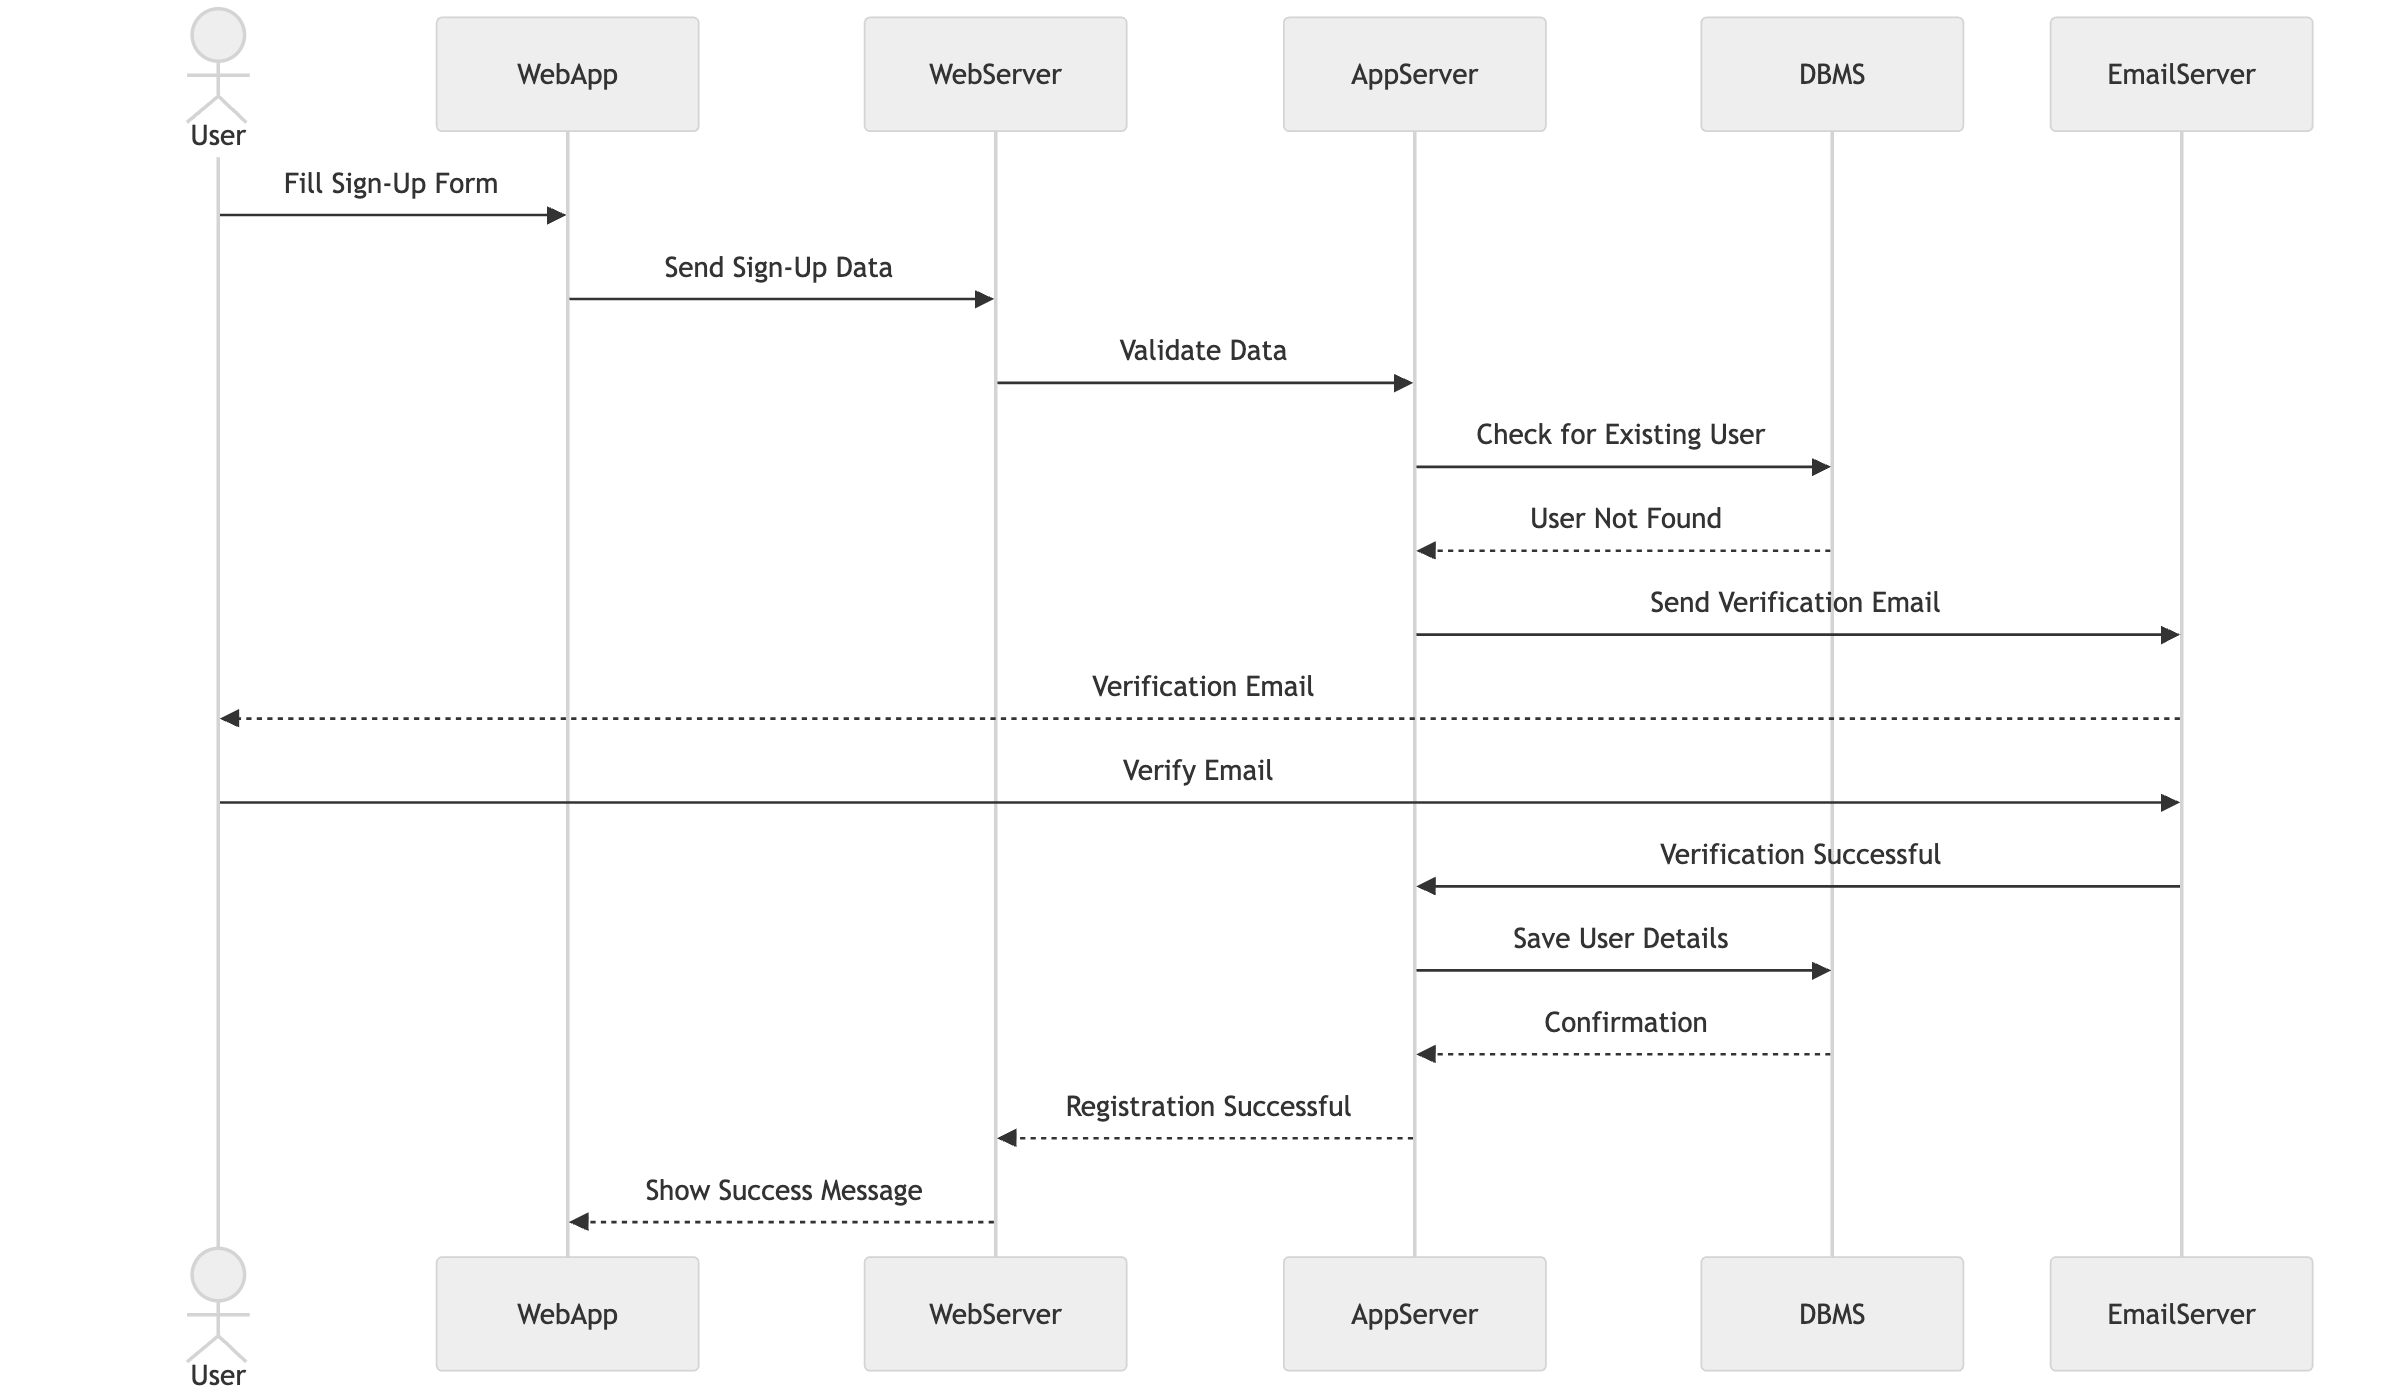
\includegraphics[width=0.82\linewidth]{JhaBhatiaSharma/imagesDD/SignUpRuntime.png}
        \caption{Runtime SignUp}
        \label{fig:signupruntime}%
    \end{center}
\end{figure}

The platform's sign-up process allows new users (students, companies, or university administrators) to register. The process is as follows:
\begin{enumerate}
    \item Through the WebApp's sign-up form, the user provides their name, email address, password, and user role.
    \item After confirming the inputs, the Web Server securely sends the data to the Application Server.
    \item The DBMS Server is used by the Application Server's Registration Manager component to search the database for duplicate records.
    \item The Email Server sends a verification email if the user is unique.
    \item The Application Server validates successful registration and saves the user's information in the database after confirming the email.
\end{enumerate}

\subsection{Login Process}
\label{subsec:login_process}

\begin{figure}[H]
    \begin{center}
        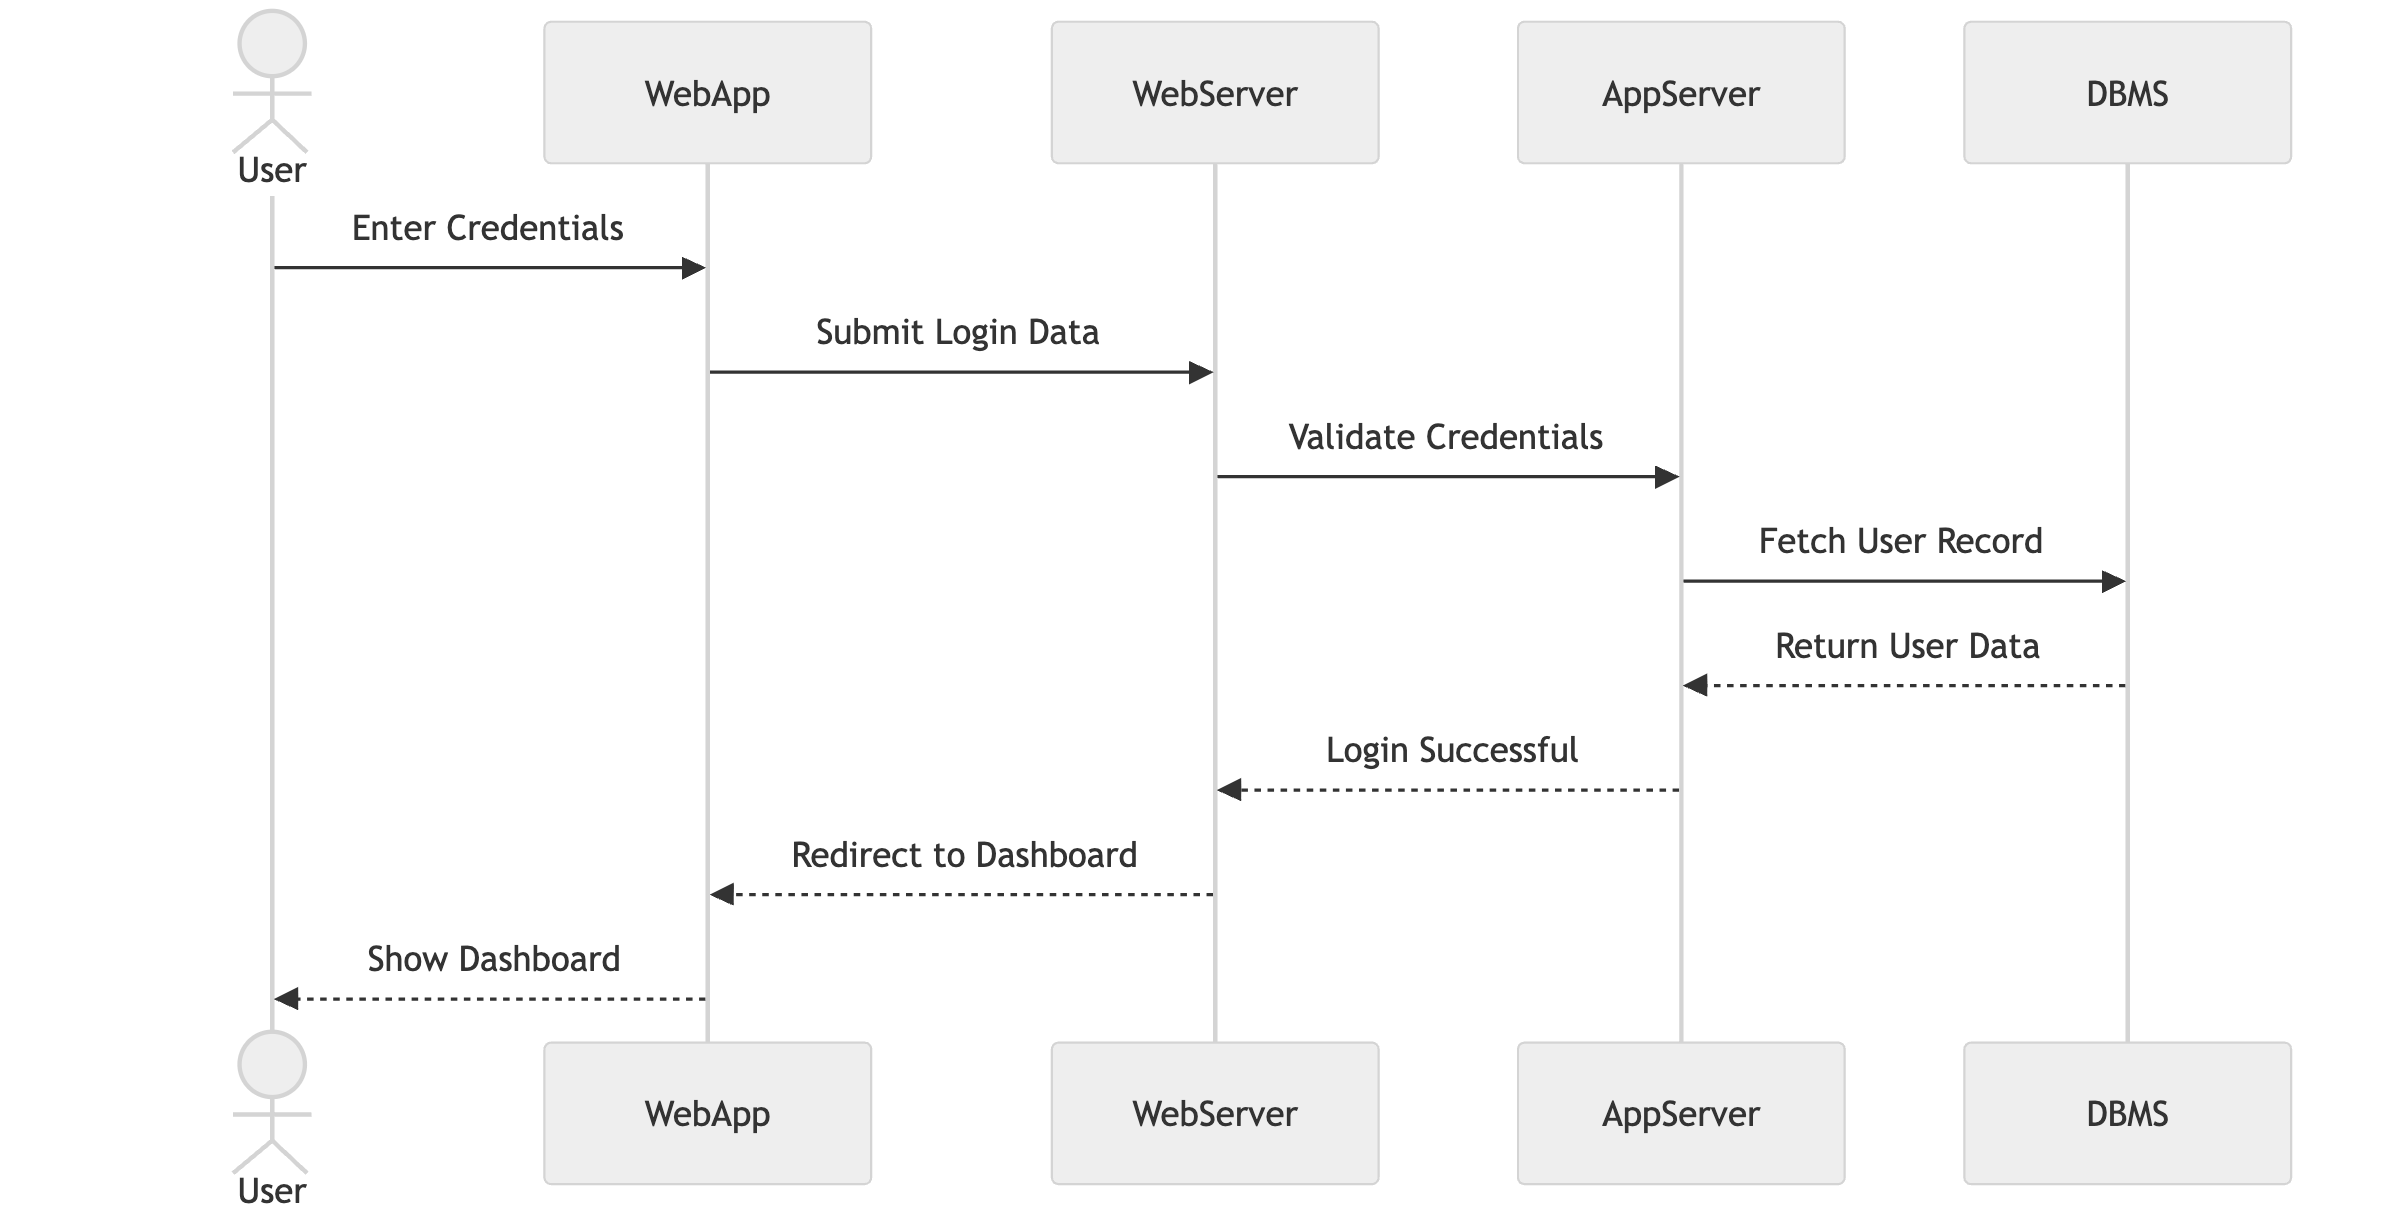
\includegraphics[width=0.82\linewidth]{JhaBhatiaSharma/imagesDD/LoginRuntime.png}
        \caption{Runtime Login}
        \label{fig:loginruntime}%
    \end{center}
\end{figure}

The login process ensures secure access for registered users. The steps are as follows:
\begin{enumerate}
    \item The user inputs their credentials on the WebApp’s login form.
    \item The Application Server receives the data safely from the Web Server.
    \item Through the DBMS Server, the Application Server's Login Manager compares the credentials against database entries.
    \item The system creates a session token and logs the user into the platform if the credentials match.
    \item To ensure easy and safe access, the user is taken to their dashboard.
\end{enumerate}

\subsection{Post Internship}
\label{subsec:post_internship}
\begin{figure}[H]
    \begin{center}
        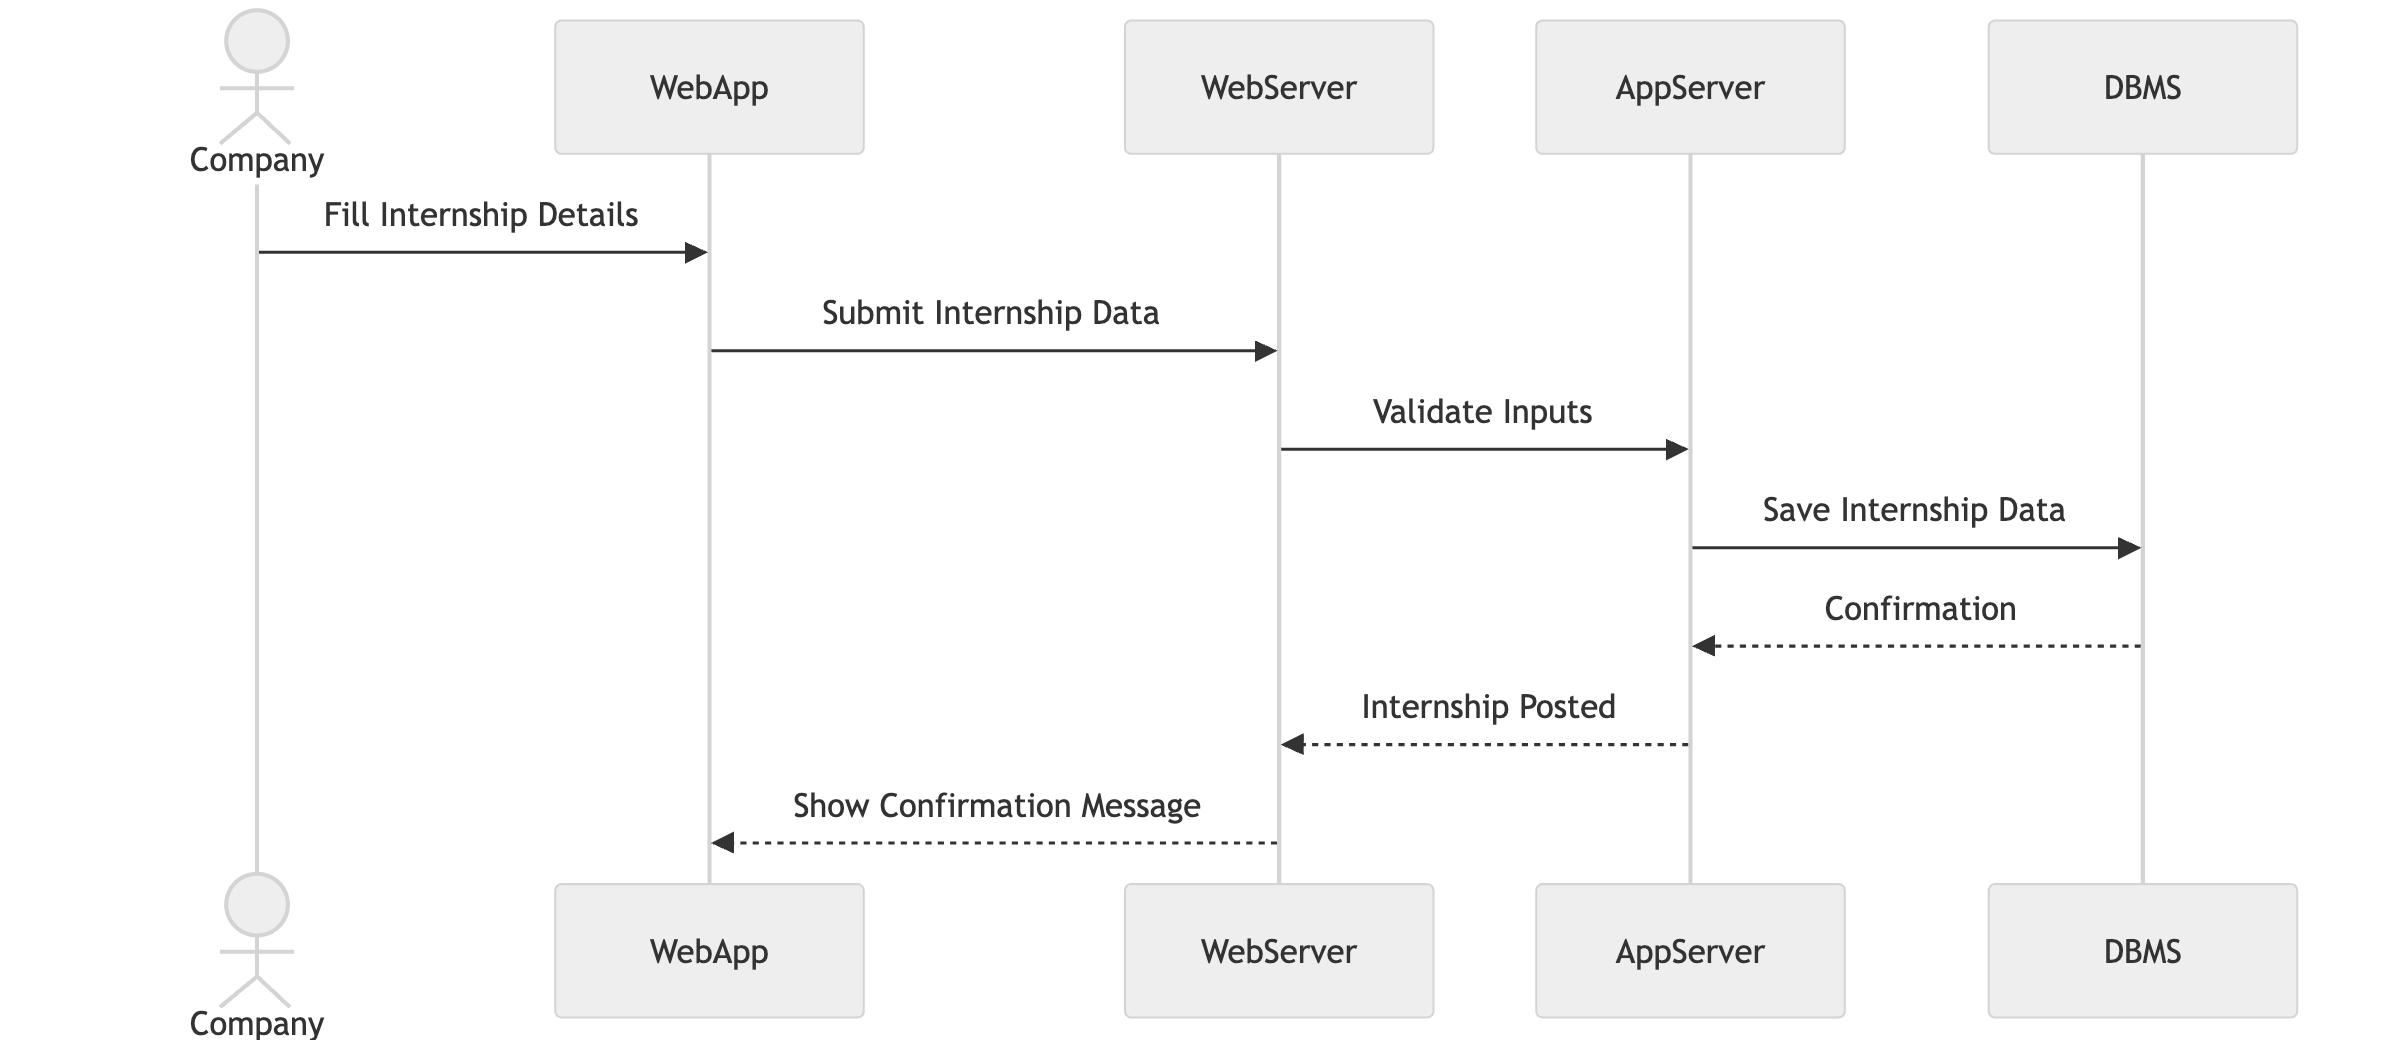
\includegraphics[width=0.82\linewidth]{JhaBhatiaSharma/imagesDD/PostInternshipRuntime.png}
        \caption{Runtime Post Internship}
        \label{fig:postinternshpruntime}%
    \end{center}
\end{figure}
Posting an internship is an essential function for company users. The process is as follows:
\begin{enumerate}
    \item By completing the internship details using the WebApp, including the job title, description, requirements, and duration, the company user starts the process.
    \item After receiving this data, the Web Server sends it to the Application Server for validation.
    \item The new internship posting is stored in the database by the Internship Manager component, which handles data processing and communication with the DBMS Server.
    \item A confirmation message is sent to the company user when the data has been successfully stored.
\end{enumerate}
This process ensures that the posted internship is immediately visible to qualified students looking for opportunities.

\subsection{Interview Management}
\label{subsec:interview_management}
\begin{figure}[H]
    \begin{center}
        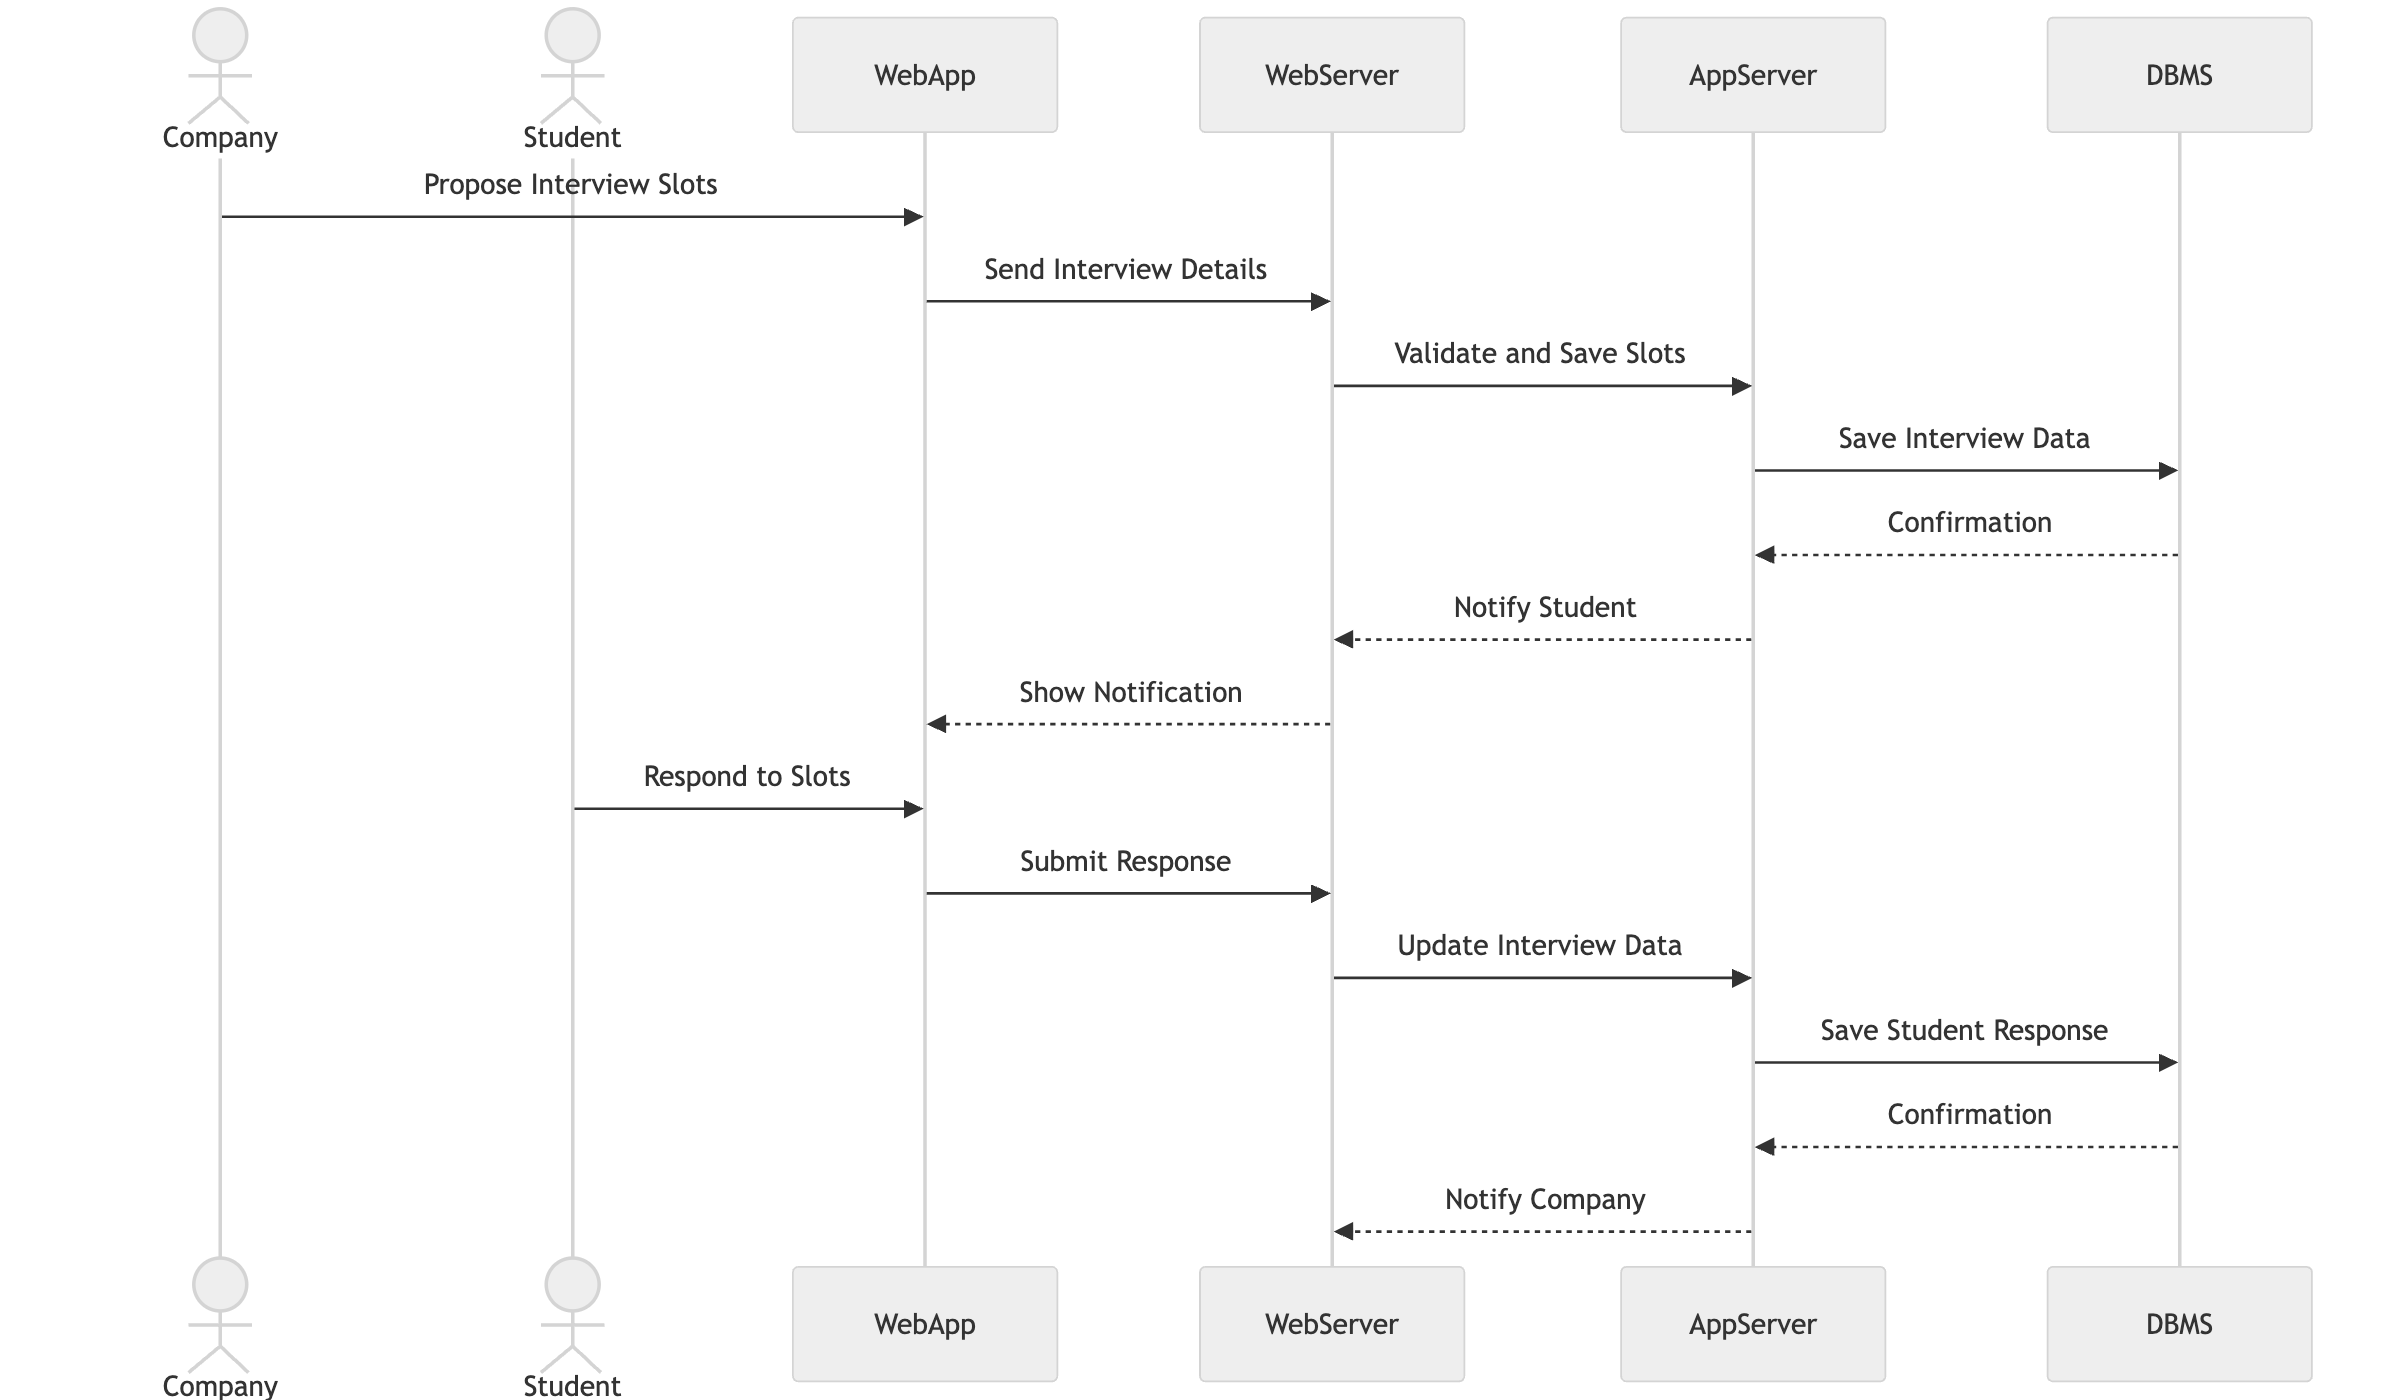
\includegraphics[width=0.82\linewidth]{JhaBhatiaSharma/imagesDD/InterviewManagementRuntime.png}
        \caption{Runtime Interview Management}
    \label{fig:interviewmanagementruntime}%
    \end{center}
\end{figure}

The interview management process streamlines scheduling and coordination between students and companies. The steps involved are:
\begin{enumerate}
    \item Employers use the WebApp to suggest interview schedules. After passing via the Web Server, the data is sent to the Application Server.
    \item The DBMS Server is used by the Interview Manager component to store the suggested timeslots in the database after verifying them.
    \item The Notification Manager and Email Server are used to inform students of the recommended timeslots.
    \item Through the WebApp, students can reply to the suggested timeslots, and the Interview Manager updates their answers in the database.
    \item The business receives notifications verifying the student's choice.
\end{enumerate}
This efficient process ensures seamless scheduling and communication for both parties.

\subsection{Complaint Handling}
\label{subsec:complaint_handling}
\begin{figure}[H]
    \begin{center}
        \includegraphics[width=0.82\linewidth]{JhaBhatiaSharma/imagesDD/ComplaintHandling.png}
        \caption{Complaint Handling}
        \label{fig:complainthandling}%
    \end{center}
\end{figure}
The complaint-handling process is designed to efficiently address user complaints. The steps are as follows:

\begin{enumerate}
    \item Complaints submitted by users via the WebApp are routed to the Web Server and subsequently to the Application Server.
    \item The Complaint Manager component uses the DBMS Server to store the complaint in the database after verifying it.
    \item After being informed of the complaint, the relevant university representative investigates it and offers a remedy.
    \item The user is informed of the resolution through the Email Server and Notification Manager.
    \item For future use, the resolution is noted in the database.
\end{enumerate}
This transparent process ensures that all complaints are handled promptly and efficiently.

\subsection{Profile Management}
\label{subsec:profile_management}
\begin{figure}[H]
    \begin{center}
        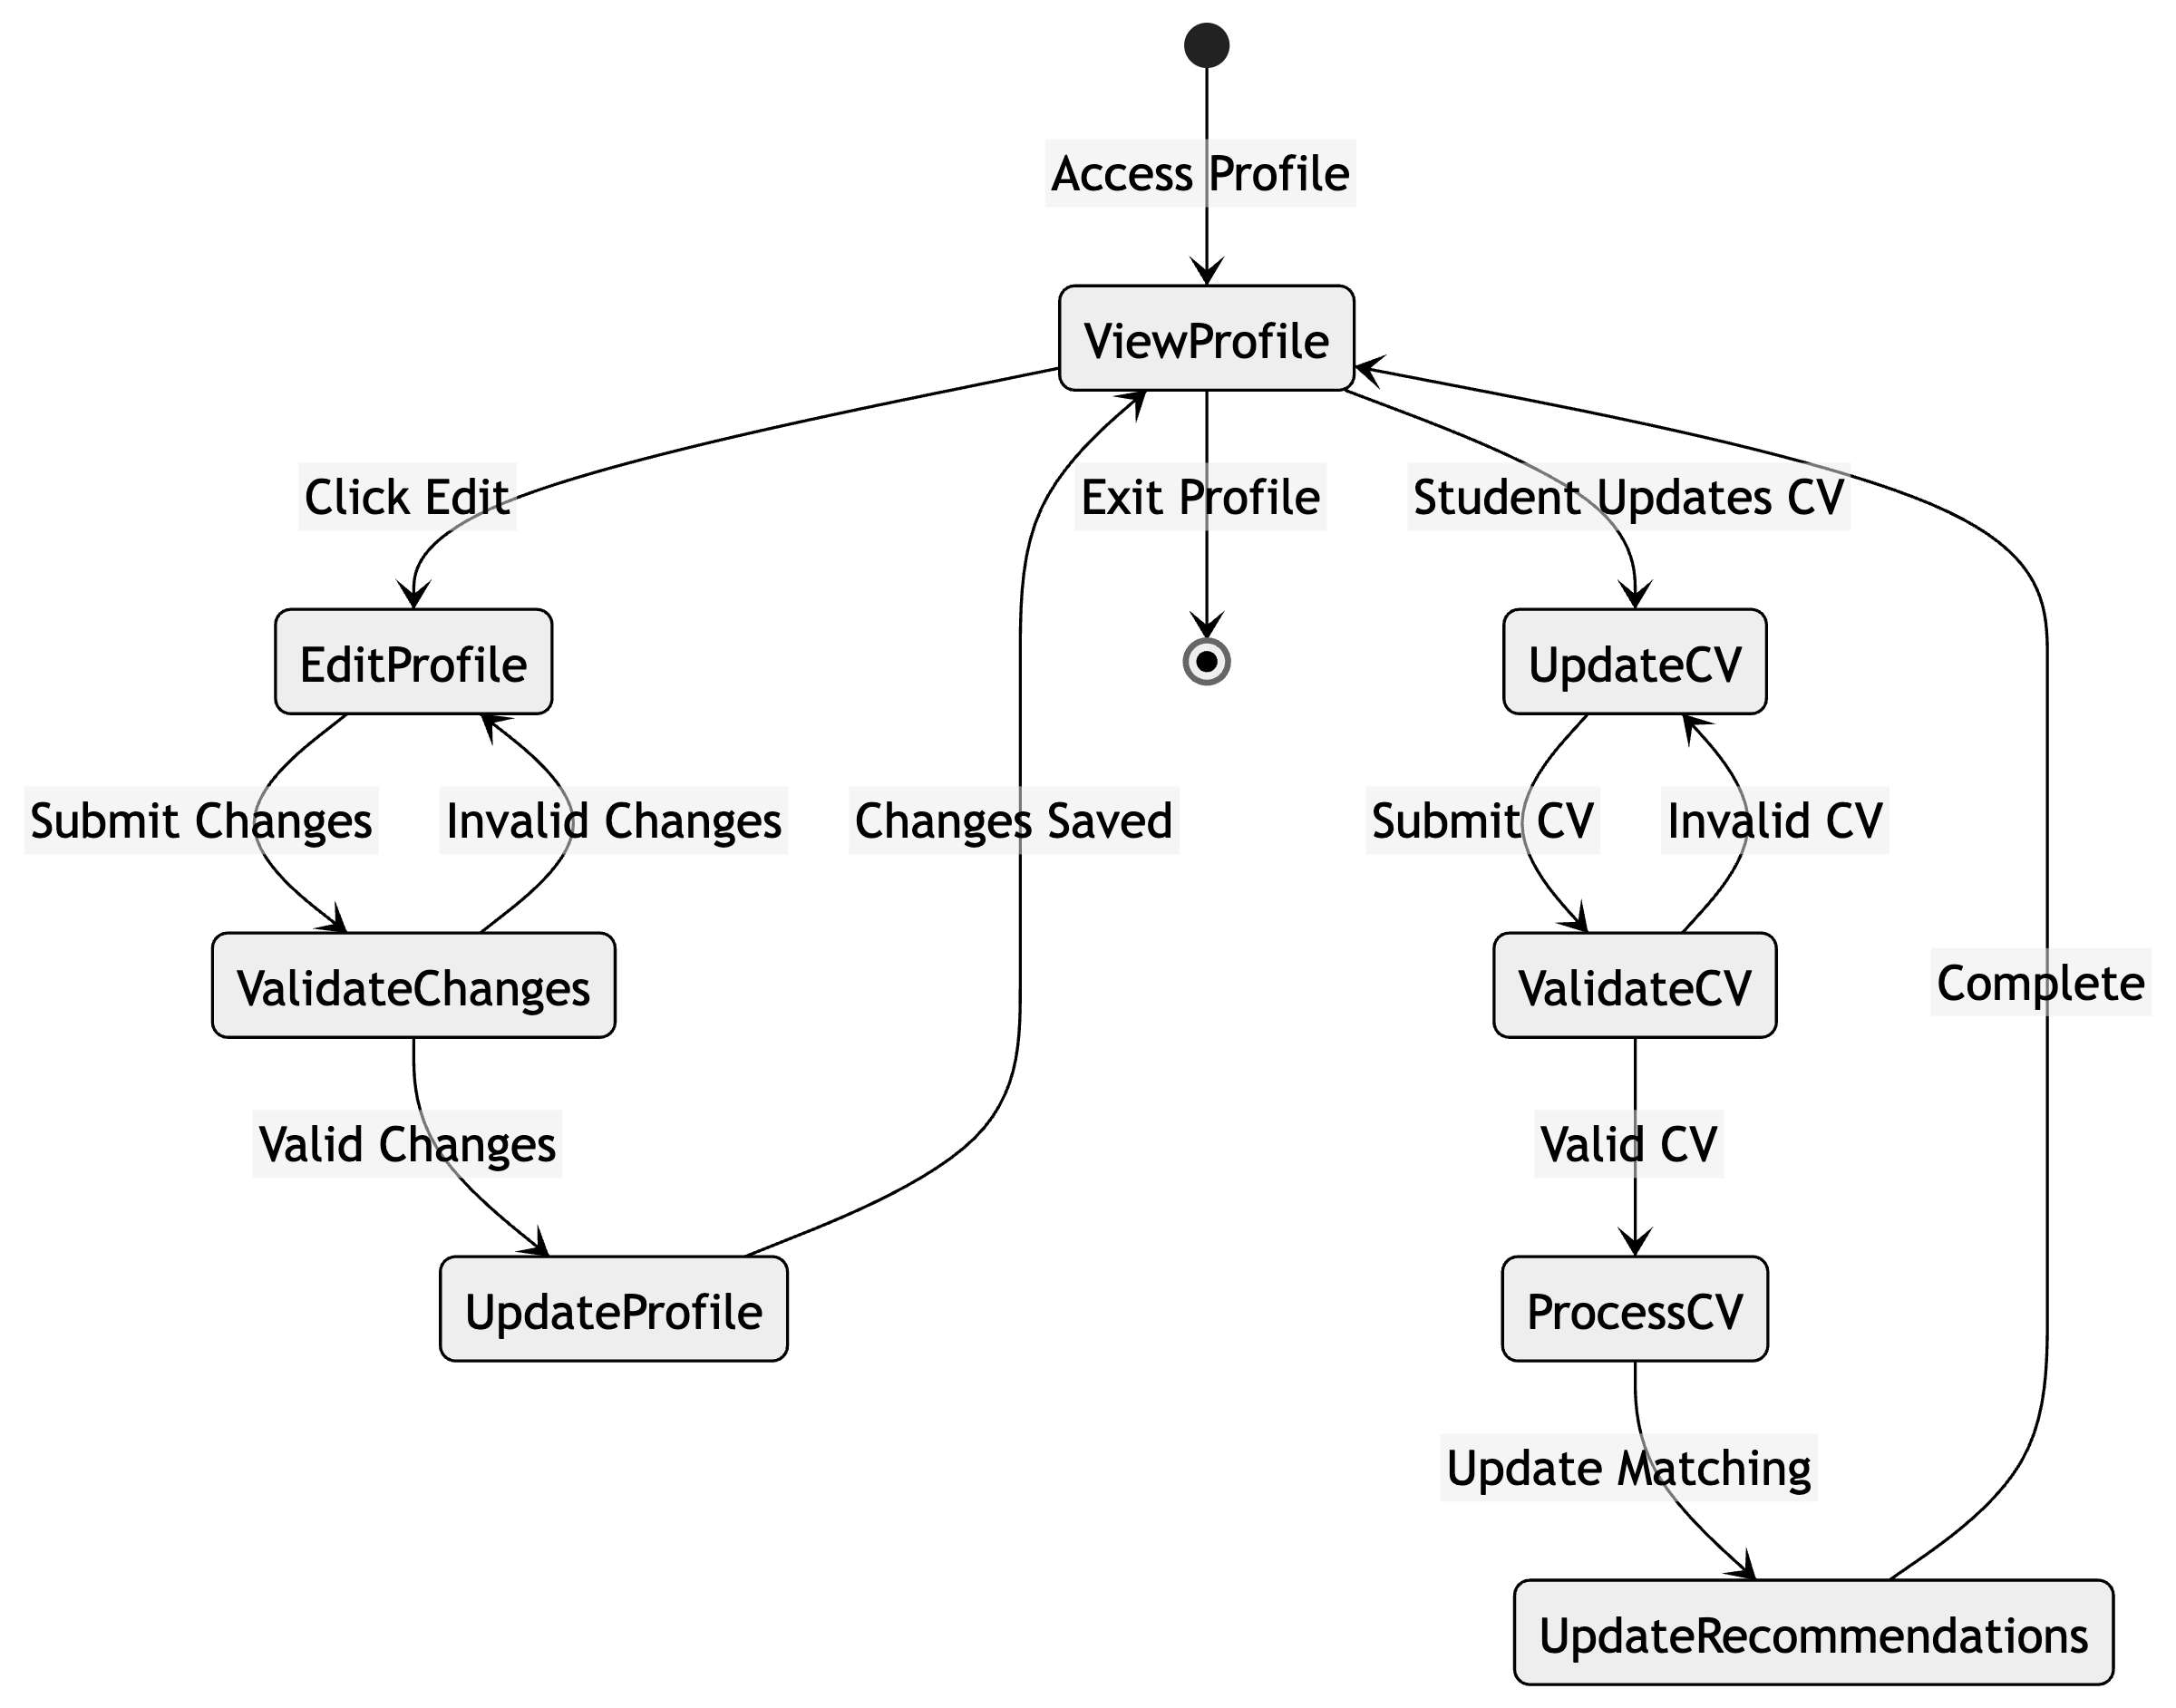
\includegraphics[width=0.82\linewidth]{JhaBhatiaSharma/imagesDD/ProfileManagement.png}
        \caption{Profile Management}
        \label{fig:profilemanagement}%
    \end{center}
\end{figure}

Profile management allows users to update and maintain their personal information. The process includes:
\begin{enumerate}
    \item Updates are started by users by inputting information including contact data, talents, and educational background on the WebApp's profile page.
    \item The Application Server receives these changes from the Web Server.
    \item In order to store the updated data in the database, the Profile Manager contacts the DBMS Server and confirms the changes.
    \item A success message is displayed to the user when the modifications have been saved.
\end{enumerate}
This feature ensures that user profiles remain up-to-date and relevant for internship matching and application processes.

\subsection{Search and Filter}
\label{subsec:search_and_filter}

\begin{figure}[H]
    \begin{center}
        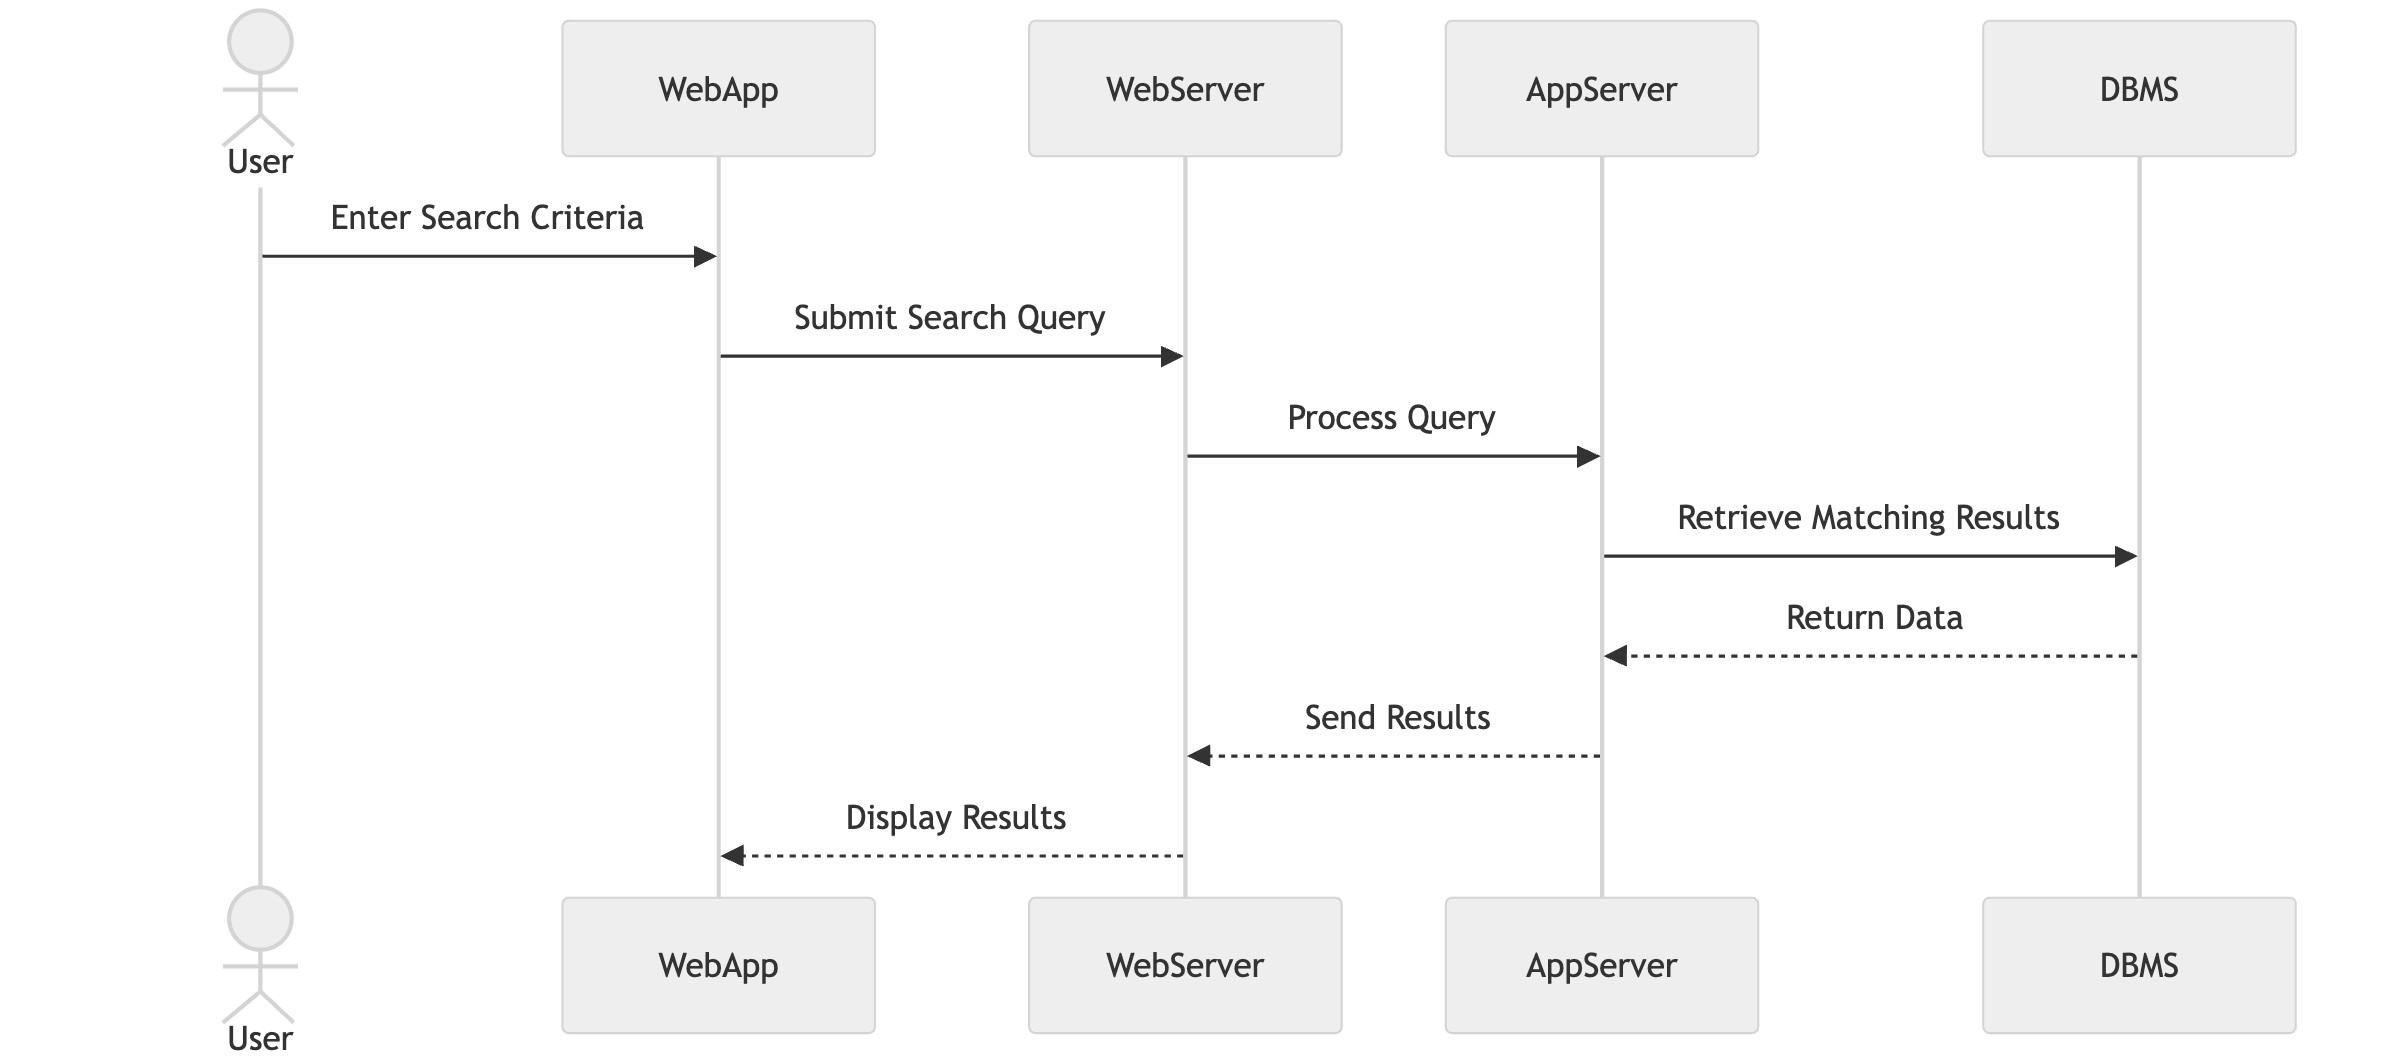
\includegraphics[width=0.82\linewidth]{JhaBhatiaSharma/imagesDD/SearchandFilter.png}
        \caption{Search and Filter}
        \label{fig:searchandfileter}%
    \end{center}
\end{figure}

The search and filter process enables users to quickly find relevant information. The workflow is as follows:
\begin{enumerate}
    \item Using the WebApp, users may search for internships by using filters like location, needed skills, and duration.
    \item These filters are sent to the Application Server by the Web Server.
    \item In order to process the query and obtain relevant results, the Search Component communicates with the DBMS Server.
    \item The WebApp receives the results from the Web Server and displays them for users to see.
\end{enumerate}
This functionality helps users efficiently navigate the platform's data and find the most relevant opportunities.

\section{Component Interfaces}
\label{subsec:component_interfaces}

\paragraph{Health Manager}
\begin{itemize}
    \item \textbf{getHealthStatus():} Verifies the health of the server and ensures it is running properly. Returns a status code and a message indicating the server status.
\end{itemize}

\paragraph{Login Manager}
\begin{itemize}
    \item \textbf{Login(String nickname, String password):} Validates user credentials and initiates a session for the user.
\end{itemize}

\paragraph{Registration Manager}
\begin{itemize}
    \item \textbf{CreateAnAccount():} Initiates the account creation process.
    \item \textbf{registerStudent(Map<String, String> studentDetails):} Registers a new student with details like name, email, and profile information.
    \item \textbf{registerRecruiter(Map<String, String> recruiterDetails):} Registers a new recruiter with details like company name, email, and profile information.
\end{itemize}

\paragraph{Internship Manager}
\begin{itemize}
    \item \textbf{addInternship(Map<String, String> internshipDetails):} enables recruiters to add a new internship following authorization validation.
    \item \textbf{deleteInternship(String internshipID):} After verifying recruiter rights, a specified internship is deleted.
    \item \textbf{fetchAllInternships(String recruiterID):} retrieves every internship that a particular recruiter has posted.
    \item \textbf{fetchInternshipById(String internshipID):} uses its ID to retrieve information on a particular internship.
\end{itemize}

\paragraph{Application Manager}
\begin{itemize}
    \item \textbf{SubmitApplication(String internshipID, String studentNickname, String resume):} gives students the opportunity to apply for a particular internship.
    \item \textbf{ViewApplications(String internshipID):} retrieves every applicant submitted for a specific internship.
    \item \textbf{UpdateApplicationStatus(String applicationID, String status):} updates a submitted application's status.
\end{itemize}

\paragraph{Interview Manager}
\begin{itemize}
    \item \textbf{ProposeInterview(String internshipID, List<Date> availableDates):} enables companies to suggest times for interviews for a particular internship.
    \item \textbf{RespondToInterview(String interviewID, String response):} gives students the option to accept or reject an invitation to an interview.
    \item \textbf{GetInterviewDetails(String interviewID):} Retrieves details about a specific interview.
\end{itemize}

\paragraph{Complaint Manager}
\begin{itemize}
    \item \textbf{SubmitComplaint(String userID, String description):} enables people to complain about a problem.
    \item \textbf{ViewComplaint(String complaintID):} brings up information on a certain complaint.
    \item \textbf{ResolveComplaint(String complaintID, String resolution):} provides an update on the complaint's status and outcome.
\end{itemize}

\paragraph{Profile Manager}
\begin{itemize}
    \item \textbf{EditProfile(String nickname, Map<String, String> updatedDetails):} Updates the user’s profile information.
    \item \textbf{ViewProfile(String nickname):} retrieves a user's profile information.
    \item \textbf{SearchProfiles(String keyword):} uses the supplied keyword to search for profiles.
\end{itemize}

\paragraph{Notification Manager}
\begin{itemize}
    \item \textbf{SendNotification(String userID, String message):} gives a user a notification.
    \item \textbf{ViewNotifications(String userID):} brings up every notification for a particular user.
\end{itemize}

\paragraph{OTP Manager}
\begin{itemize}
    \item \textbf{requestOTP(String email):} Requests an OTP for email-based authentication.
    \item \textbf{verifyOTP(String email, String otp):} confirms the OTP supplied for email authentication.
\end{itemize}

\paragraph{Token Manager}
\begin{itemize}
    \item \textbf{generateAccessToken(String email, String userType):} confirms the OTP supplied for email authentication.
\end{itemize}

\paragraph{Dashboard Manager}
\begin{itemize}
    \item \textbf{GetDashboardData(String userID):} gives the user who is logged in a summary of the dashboard.
    \item \textbf{ViewStatistics(String userID):} retrieves statistics information pertinent to the user's actions.
\end{itemize}

\section{Architectural Styles and Patterns}
\label{subsec:architectural_styles_patterns}

\subsection{Layered Architecture}
\paragraph{Front-End Layer}
\begin{itemize}
    \item Implements responsive web interfaces for three distinct user types:
    \begin{itemize}
        \item \textbf{Student Portal:} focuses on managing applications, searching for internships, and maintaining profiles.
        \item \textbf{Company Portal:} manages prospects, reviews applications, and posts internships.
        \item \textbf{Admin Portal:} offers system monitoring, complaint handling, and oversight tools.
    \end{itemize}
    \item Uses modern web technologies with responsive design principles.
    \item carries out state management and client-side validation.
\end{itemize}

\paragraph{Services Layer (Business Logic)}
\begin{itemize}
    \item \textbf{User Management Service:} manages user profiles, rights, authorization, and authentication.
    \item \textbf{Matching Engine Service:} carries out the filtering and sorting of results, processes search queries, and applies sophisticated algorithms for matching internship students.
    \item \textbf{Recommendation System:} evaluates internship requirements and student profiles to provide tailored recommendations that are updated in response to user interactions.
    \item \textbf{Interview Management Service:} oversees the scheduling of interviews, keeps track of interview status updates, and collects feedback.
\end{itemize}

\paragraph{Data Layer}
\begin{itemize}
    \item \textbf{Database Management System:} keeps organized information such as applications, internships, and user profiles. preserves relationship mappings and guarantees the consistency and integrity of data.
    \item \textbf{File Storage System:} oversees the safe uploading and downloading of files, manages the storage of documents (certificates, resumes), and applies file versioning.
\end{itemize}

\subsection{Client-Server Architecture}
\paragraph{Client Side Implementation}
\begin{itemize}
    \item uses a browser-based responsive user interface that can be adjusted to fit various screen sizes and devices.
    \item applies client-side validations and offers a consistent user experience.
\end{itemize}

\paragraph{Real-Time Updates}
\begin{itemize}
    \item Uses WebSocket connections for instant notifications.
    \item Updates UI states that preserve synchronized views without requiring a page refresh.
\end{itemize}

\paragraph{Server Side Implementation}
\begin{itemize}
    \item \textbf{RESTful API Services:} handles request/response processing, API versioning, and the implementation of defined HTTP endpoints.
    \item \textbf{Backend Processing:} Executes business logic operations, processes data transformations, and manages system state.
\end{itemize}

\subsection{Event-Driven Architecture}
\paragraph{Event Publishers}
\begin{itemize}
    \item \textbf{Application System:} activates notification workflows, creates events for status changes, and updates relevant entities.
    \item \textbf{Interview System:} creates events, notifies users of reminders, and modifies calendar integrations.
    \item \textbf{Complaint System:} Notifies the appropriate administrators, initiates escalation events, and modifies the tracking status.
\end{itemize}

\paragraph{Event Subscribers}
\begin{itemize}
    \item \textbf{Notification Service:} sends emails and alerts, handles event notifications, and modifies user dashboards.
    \item \textbf{Analytics Service:} maintains reporting metrics, creates usage statistics, and keeps track of system occurrences.
\end{itemize}

\subsection{Design Patterns}
\label{subsec:design_patterns}

\paragraph{1. Model-View-Controller (MVC)}
\begin{itemize}
    \item \textbf{Models:}
    \begin{itemize}
        \item \textbf{User Model:}
        \begin{itemize}
            \item Base user properties and behaviors.
            \item Specialized student, company, and admin classes.
            \item Data validation rules.
        \end{itemize}
        \item \textbf{Application Model:}
        \begin{itemize}
            \item Application states and transitions.
            \item Document attachments.
            \item Status tracking.
        \end{itemize}
        \item \textbf{Internship Model:}
        \begin{itemize}
            \item Position details and requirements.
            \item Application management.
            \item Scheduling information.
        \end{itemize}
    \end{itemize}
    \item \textbf{Views:}
    \begin{itemize}
        \item \textbf{User Interfaces:}
        \begin{itemize}
            \item Role-specific dashboards.
            \item Form components.
            \item Interactive elements.
        \end{itemize}
        \item \textbf{Data Presentation:}
        \begin{itemize}
            \item Lists and tables.
            \item Search results.
            \item Statistical reports.
        \end{itemize}
    \end{itemize}
    \item \textbf{Controllers:}
    \begin{itemize}
        \item \textbf{Authentication Controller:}
        \begin{itemize}
            \item Login/logout handling.
            \item Session management.
            \item Access control.
        \end{itemize}
        \item \textbf{Application Controller:}
        \begin{itemize}
            \item Process submissions.
            \item Status updates.
            \item Document handling.
        \end{itemize}
    \end{itemize}
\end{itemize}

\paragraph{2. Observer Pattern}
\begin{itemize}
    \item \textbf{Subject Components:}
    \begin{itemize}
        \item \textbf{Internship Posting System:}
        \begin{itemize}
            \item Notifies matched students.
            \item Updates search results.
            \item Triggers recommendations.
        \end{itemize}
        \item \textbf{Application Processing:}
        \begin{itemize}
            \item Updates stakeholders.
            \item Triggers next steps.
            \item Maintains status logs.
        \end{itemize}
    \end{itemize}
    \item \textbf{Observer Components:}
    \begin{itemize}
        \item \textbf{Student Notifications:}
        \begin{itemize}
            \item New matching internships.
            \item Application updates.
            \item Interview schedules.
        \end{itemize}
        \item \textbf{Company Notifications:}
        \begin{itemize}
            \item New applications.
            \item Interview confirmations.
            \item Status changes.
        \end{itemize}
    \end{itemize}
\end{itemize}

\paragraph{3. Factory Pattern}
\begin{itemize}
    \item \textbf{User Factory:}
    \begin{itemize}
        \item Creates appropriate user types.
        \item Initializes role-specific properties.
        \item Sets up required relationships.
    \end{itemize}
    \item \textbf{Document Factory:}
    \begin{itemize}
        \item Generates different document types.
        \item Handles format conversions.
        \item Creates appropriate storage entries.
    \end{itemize}
\end{itemize}

\paragraph{4. State Pattern}
\begin{itemize}
    \item \textbf{Application States:}
    \begin{itemize}
        \item Submitted.
        \item Under Review.
        \item Interview Scheduled.
        \item Accepted/Rejected.
        \item Completed.
    \end{itemize}
    \item \textbf{Complaint States:}
    \begin{itemize}
        \item Filed.
        \item Under Investigation.
        \item Resolved.
        \item Closed.
        \item Escalated.
    \end{itemize}
\end{itemize}

\paragraph{5. Strategy Pattern}
\begin{itemize}
    \item \textbf{Matching Strategies:}
    \begin{itemize}
        \item Skills-based matching.
        \item Location-based matching.
        \item Experience-level matching.
        \item Industry-specific matching.
    \end{itemize}
    \item \textbf{Search Strategies:}
    \begin{itemize}
        \item Keyword search.
        \item Filter-based search.
        \item Category-based search.
        \item Combined search approaches.
    \end{itemize}
\end{itemize}

\paragraph{Benefits of Implementing Design Patterns:}
\begin{itemize}
    \item Clear separation of concerns.
    \item Maintainable and scalable codebase.
    \item Robust error handling.
    \item Secure data management.
    \item Efficient performance.
    \item Real-time responsiveness.
    \item Consistent user experience.
\end{itemize}

\section{Other Design Decisions}
\label{sec:other_design_decisions}

\subsection{Availability}
\label{subsec:availability}
\begin{itemize}
    \item Redundant systems guarantee uninterrupted, 24/7 platform operation.
    \item During interruptions, a failover mechanism allows for automatic shift to backup systems.
    \item Data integrity is guaranteed by error handling procedures.
    \item System recovery procedures after failures.
    \item Transaction integrity for important procedures such as scheduling interviews and submitting applications.
\end{itemize}

\subsection{Scalability}
\label{subsec:scalability}
\begin{itemize}
    \item Front-end layer scalability for multiple user portals (Student, Company, Admin).
    \item Services layer that can scale independently based on demand:
    \begin{itemize}
        \item User Management Service.
        \item Matching Engine.
        \item Recommendation System.
        \item Interview Management Service.
    \end{itemize}
    \item Systems for databases and storage that can handle increasing amounts of data.
    \item API-first approach enabling future mobile app development.
\end{itemize}

\subsection{Security}
\label{subsec:security}
\begin{itemize}
    \item Robust authentication systems for user verification.
    \item authorization for sensitive operations based on roles.
    \item End-to-end data encryption.
    \item GDPR compliance measures.
    \item Secure document storage and handling.
    \item routine security monitoring and audits.
\end{itemize}

\subsection{Notification Handling}
\label{subsec:notification_handling}
\begin{itemize}
    \item Notifications in real time when the status of an application changes.
    \item Interview scheduling alerts.
    \item Complaint status updates.
    \item Notifications about important occurrences via email.
    \item Integration of a calendar to schedule interviews.
    \item Platform-wide announcements capability.
\end{itemize}

\subsection{Document Management}
\label{subsec:document_management}
\begin{itemize}
    \item Certificates, formal documents, and resumes should all be stored securely.
    \item Version control for user documents.
    \item Document validation and verification.
    \item Format standardization.
    \item Access control based on user roles.
    \item Automated capacity for processing documents.
\end{itemize}

\subsection{Data Persistence}
\label{subsec:data_persistence}
\begin{itemize}
    \item Centralized database for core functionality:
    \begin{itemize}
        \item User profiles.
        \item Internship listings.
        \item Applications.
        \item Interview records.
        \item Complaints.
    \end{itemize}
    \item File storage system for documents.
    \item Data backup and recovery systems.
    \item Audit logging for critical operations.
    \item Data retention policies compliance.
\end{itemize}

\subsection{Performance Optimization}
\label{subsec:performance_optimization}
\begin{itemize}
    \item Page load optimization (\textless 5 seconds).
    \item Search results delivery (\textless 2 seconds).
    \item File upload handling (\textless 10 seconds for 10MB).
    \item Real-time updates (\textless 1 second).
    \item Concurrent user support (up to 50 users).
    \item Database transaction optimization (10 transactions per second).
\end{itemize}

\paragraph{Alignment with Platform Goals:}
These design decisions align with the platform's core requirements while ensuring:
\begin{itemize}
    \item Reliable service delivery.
    \item Secure data handling.
    \item Efficient performance.
    \item User satisfaction.
    \item System maintainability.
    \item Regulatory compliance.
    \item Future scalability.
\end{itemize}



    \chapter{User Interface Design}
    \label{ch:user_interface_design}%
    \section{External interface requirements}
\label{sec:external_interface_requirements}%

\subsection{User Interfaces}
\label{subsec:User_interfaces}%

Students, businesses, and university administrators will be able to access the InternHub - Students \& Companies (S\&C) platform's \textbf{user interface} via a \textbf{responsive web application} on any device with a current web browser and an internet connection.
\subsubsection{Authentication Interface}
\begin{enumerate}
    \item User login and registration.
    \item Password reset functionality.
    \item Multi-factor authentication (optional).
\end{enumerate}

\begin{figure}[H]
    \centering
    \begin{minipage}{0.33\textwidth}
        \centering
        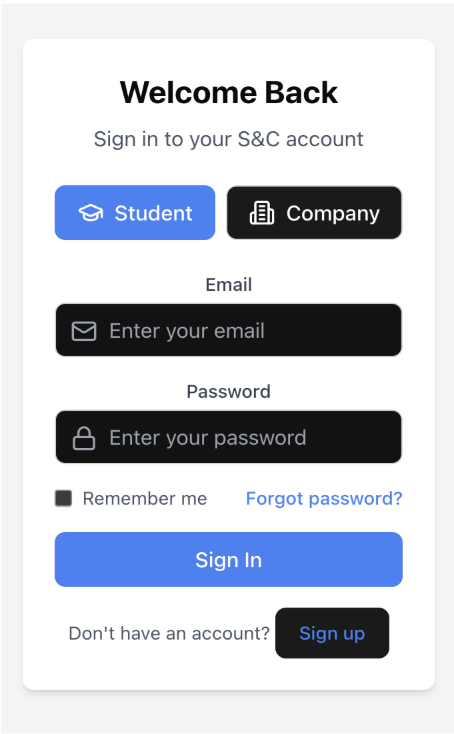
\includegraphics[width=\linewidth]{JhaBhatiaSharma/Images/Mockups/Login.png}
        \caption{Login mockup.}
        \label{fig:login_mockup}
    \end{minipage}
    \hspace{1cm} % Adjust the space between images
    \begin{minipage}{0.33\textwidth}
        \centering
        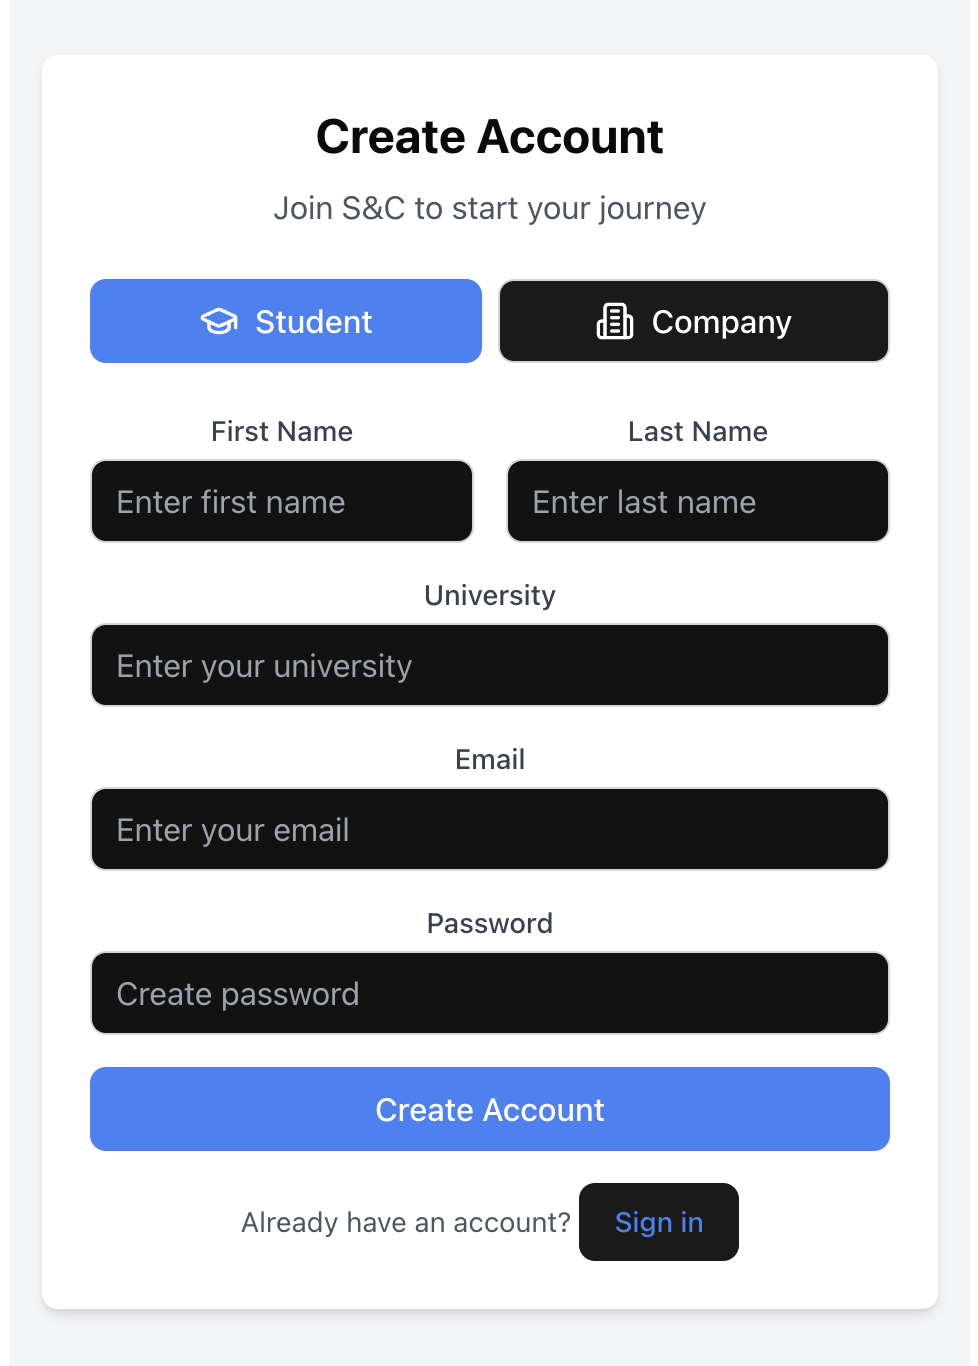
\includegraphics[width=\linewidth]{JhaBhatiaSharma/Images/Mockups/SignUp.png}
        \caption{SignUp mockup.}
        \label{fig:signup_mockup}
    \end{minipage}
\end{figure}



\subsubsection{Student Interface}
\begin{enumerate}
    \item \textbf{Dashboard Overview:} Shows notifications, recommended internships, and active applications.
    \item \textbf{Profile Management:} Add or update qualifications and edit personal information.
    \item \textbf{CV Builder:} Use built-in templates to create and manage resumes.
    \item \textbf{Internship Search:} Look for and select internships according to talents, domain, and location.
    \item \textbf{Application Tracker:} Check the progress of applications that have been submitted.
    \item \textbf{Interview Calendar:} Organize interview dates with the calendar feature.
    \item \textbf{Messaging System:} Interact with administrators and businesses.
\end{enumerate}

\begin{figure}[H]
    \begin{center}
        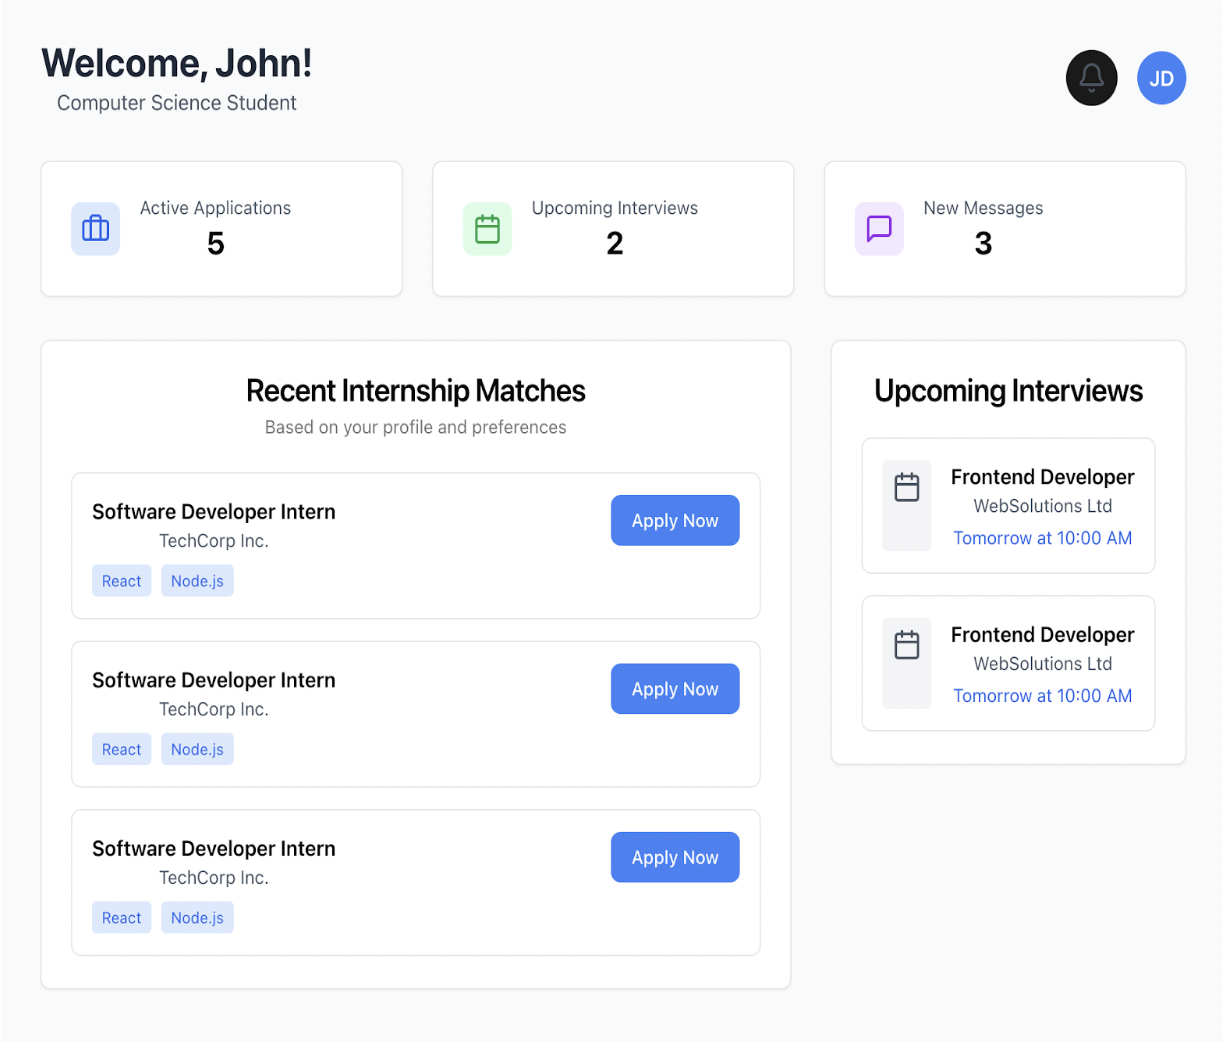
\includegraphics[width=0.82\linewidth]{JhaBhatiaSharma/Images/Mockups/StudentInterface.png}
        \caption{Student Interface Diagram}
        \label{fig:StudentInterface}%
    \end{center}
\end{figure}

\subsubsection{Company Interface}
\begin{enumerate}
    \item \textbf{Dashboard Overview:} Displays applications, postings, and other data.
    \item \textbf{Management of Company Profiles:} Modify logos and company information.
    \item \textbf{Management of Internship Postings:} Produce and oversee internship advertisements.
    \item \textbf{Managing Candidates:} Examine applications and create a shortlist of applicants.
    \item \textbf{Interview Scheduler:} Use a scheduling tool to plan and monitor interviews.
    \item \textbf{Analytics Dashboard:} Access information on posting engagement and candidate performance.
\end{enumerate}

\begin{figure}[H]
    \begin{center}
        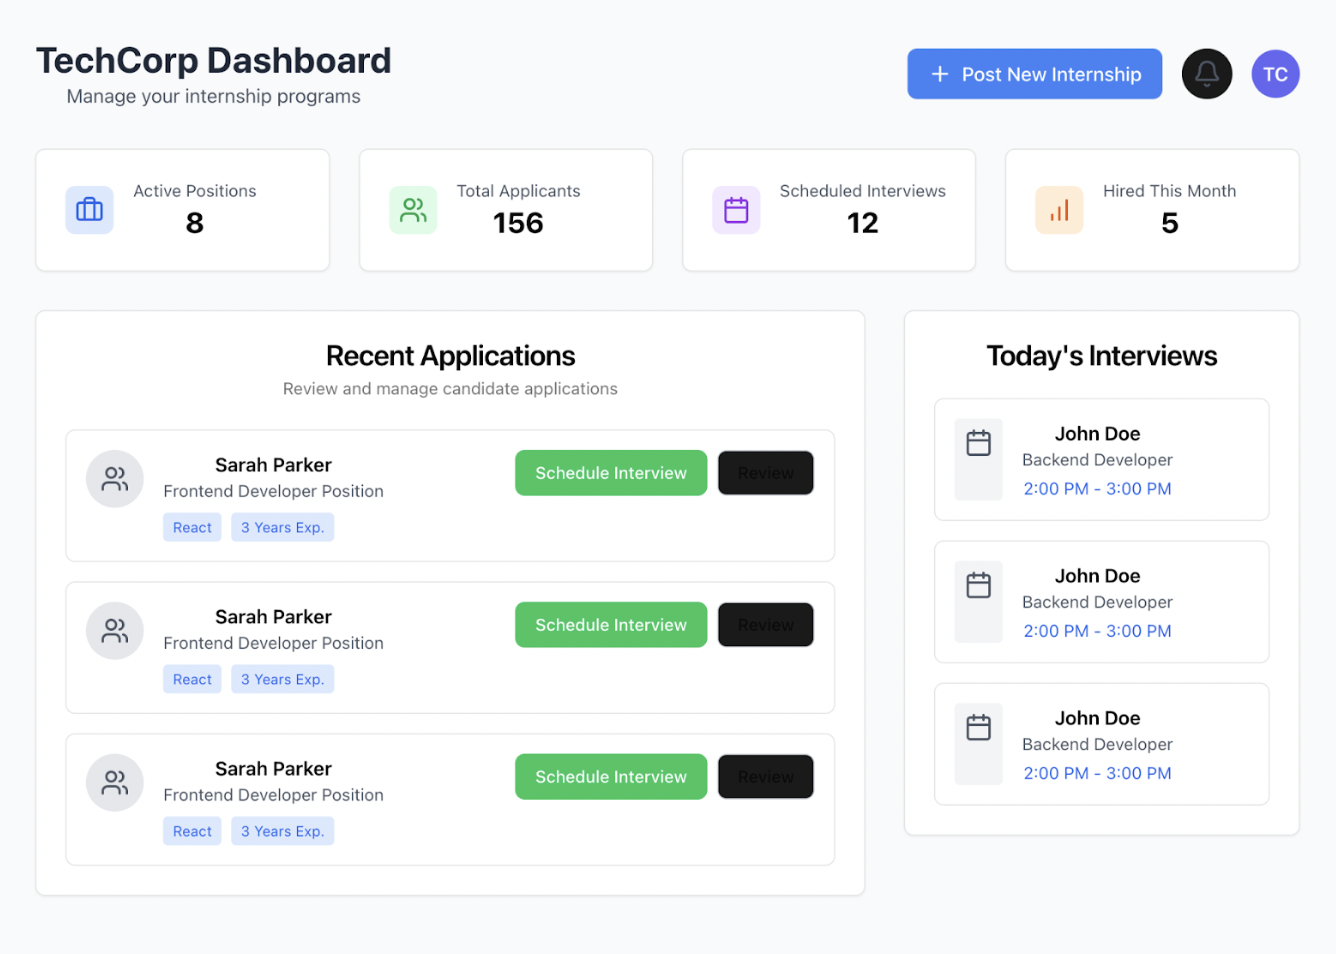
\includegraphics[width=0.82\linewidth]{JhaBhatiaSharma/Images/Mockups/CompanyInterface.png}
        \caption{Company Interface Diagram}
        \label{fig:CompanyInterface}%
    \end{center}
\end{figure}

\subsubsection{Administrator Interface}
\begin{enumerate}
    \item \textbf{System Overview:} Keep an eye on the status and activities of the platform.
    \item \textbf{User Management:} Oversee users, including administrators, businesses, and students.
    \item \textbf{Handling Complaints:} Examine and address complaints that have been submitted.
    \item \textbf{Report Creation:} Produce reports on internship progress and platform usage.
    \item \textbf{Configuration Settings:} Modify settings for the entire system.
\end{enumerate}

\begin{figure}[H]
    \begin{center}
        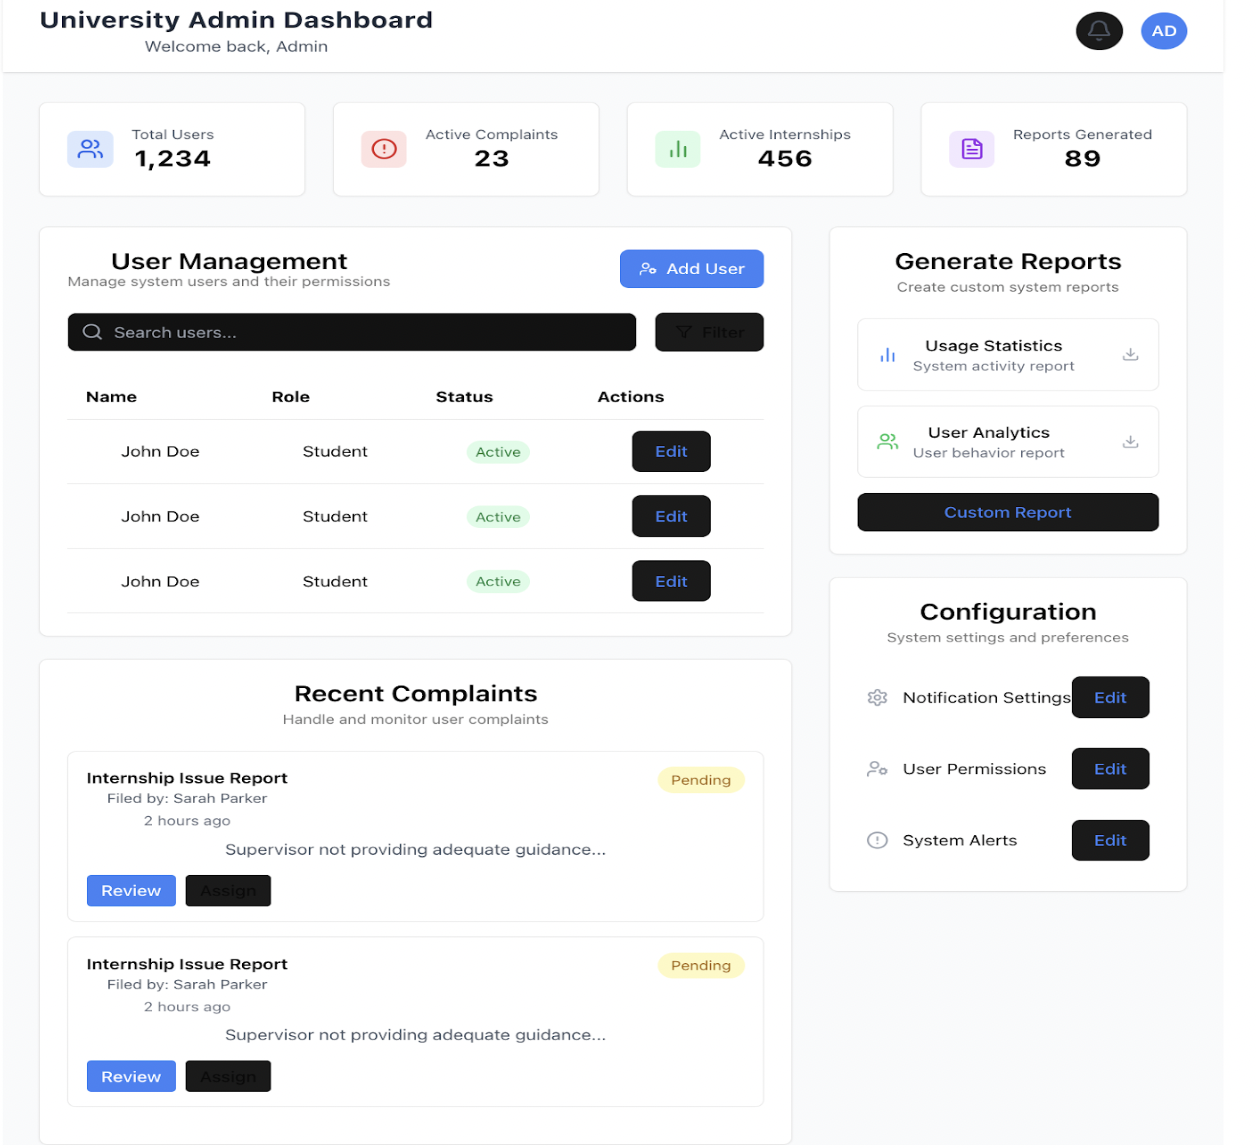
\includegraphics[width=0.82\linewidth]{JhaBhatiaSharma/Images/Mockups/AdminInterface.png}
        \caption{Administrator Interface Diagram}
        \label{fig:AdministratorInterface}%
    \end{center}
\end{figure}

\subsection{Hardware Interfaces}
\label{subsec:hardware_interfaces}%

\begin{itemize}
    \item Compatible with both desktop and mobile web browsers available today.
    \item Minimum screen resolution: 1280x720.
    \item Supports mobile devices with touch interfaces.
    \item Features for uploading and downloading resumes, job descriptions, and feedback files.
\end{itemize}

\subsection{Software Interfaces}
\label{subsec:software_interfaces}%

\begin{itemize}
    \item \textbf{Database Management System:} Stores user information, internships, and system logs.
    \item \textbf{Email Server:} Provides emails for confirmation and notifications.
    \item \textbf{File Storage System:} Manages uploaded documents, including resumes.
    \item \textbf{Authentication System:} Manages role-based access and user login.
    \item \textbf{Analytics Engine:} Produces usage reports and offers insights.
\end{itemize}


\subsection{Communication Interfaces}
\label{subsec:communication_interfaces}%

\begin{itemize}
    \item \textbf{HTTPS Protocol:} Ensures secure communication between users and the platform.
    \item \textbf{RESTful API:} Enables seamless communication between the front-end and back-end systems.
    \item \textbf{WebSocket Connections:} Supports real-time notifications for updates and alerts.
    \item \textbf{Email SMTP:} Manages email correspondence for notifications and alerts.
\end{itemize}

\section{Functional Requirements}
\label{sec:functional_requirements}%

\subsection{Requirements Lists}
\label{subsec:requirements3}%
\newcounter{req}
\setcounter{req}{1}
\newcommand{\creq}{\thereq\stepcounter{req}}

% Functional Requirements for F1
\subsubsection{F1. User Management}
\begin{center}
    \begin{longtable}{ |l|p{0.9\linewidth}| }
        \hline
        \textbf{ID} & \textbf{Description} \\
        \hline
        F1.1 & The system shall allow students, companies, and university administrators to register with verified email addresses. \\
        \hline
        F1.2 & The system shall provide secure authentication with optional two-factor verification. \\
        \hline
        F1.3 & The system shall allow users to update their profile information including contact details and preferences. \\
        \hline
        F1.4 & The system shall enforce role-based access control for students, companies, and administrators. \\
        \hline
        F1.5 & The system shall support password reset functionality with email verification. \\
        \hline
        F1.6 & The system shall maintain audit logs of all user authentication activities. \\
        \hline
        F1.7 & The system shall allow users to manage notification preferences. \\
        \hline
        F1.8 & The system shall enforce strong password policies. \\
        \hline
    \end{longtable}
\end{center}

% Functional Requirements for F2
\subsubsection{F2. CV Management}
\begin{center}
    \begin{longtable}{ |l|p{0.9\linewidth}| }
        \hline
        \textbf{ID} & \textbf{Description} \\
        \hline
        F2.1 & The system shall provide customizable CV templates for students. \\
        \hline
        F2.2 & The system shall allow students to create and store multiple versions of their CVs. \\
        \hline
        F2.3 & The system shall enable students to update their CVs at any time. \\
        \hline
        F2.4 & The system shall allow students to control CV visibility to specific companies. \\
        \hline
        F2.5 & The system shall provide a skill management interface for students. \\
        \hline
        F2.6 & The system shall validate skill entries against a standardized skill database. \\
        \hline
        F2.7 & The system shall support document upload for certificates and portfolios. \\
        \hline
        F2.8 & The system shall track CV view statistics for students. \\
        \hline
    \end{longtable}
\end{center}

% Functional Requirements for F3
\subsubsection{F3. Internship Management}
\begin{center}
    \begin{longtable}{ |l|p{0.9\linewidth}| }
        \hline
        \textbf{ID} & \textbf{Description} \\
        \hline
        F3.1 & The system shall allow companies to create detailed internship postings. \\
        \hline
        F3.2 & The system shall provide an application tracking system for companies. \\
        \hline
        F3.3 & The system shall automatically notify students of application status changes. \\
        \hline
        F3.4 & The system shall provide advanced search and filtering capabilities. \\
        \hline
        F3.5 & The system shall allow companies to set application deadlines. \\
        \hline
        F3.6 & The system shall enable bulk application processing for companies. \\
        \hline
        F3.7 & The system shall support multiple rounds of application review. \\
        \hline
        F3.8 & The system shall maintain a history of all internship postings. \\
        \hline
    \end{longtable}
\end{center}

% Functional Requirements for F4
\subsubsection{F4. Interview Management}
\begin{center}
    \begin{longtable}{ |l|p{0.9\linewidth}| }
        \hline
        \textbf{ID} & \textbf{Description} \\
        \hline
        F4.1 & The system shall provide a calendar interface for interview scheduling. \\
        \hline
        F4.2 & The system shall track interview status and progress. \\
        \hline
        F4.3 & The system shall collect structured feedback from both parties. \\
        \hline
        F4.4 & The system shall send automated interview reminders. \\
        \hline
        F4.5 & The system shall support virtual interview link generation. \\
        \hline
        F4.6 & The system shall allow rescheduling with mutual agreement. \\
        \hline
        F4.7 & The system shall maintain interview history. \\
        \hline
        F4.8 & The system shall support multiple interview rounds. \\
        \hline
    \end{longtable}
\end{center}

% Functional Requirements for F5
\subsubsection{F5. Recommendation System}
\begin{center}
    \begin{longtable}{ |l|p{0.9\linewidth}| }
        \hline
        \textbf{ID} & \textbf{Description} \\
        \hline
        F5.1 & The system shall match students with internships based on skills alignment. \\
        \hline
        F5.2 & The system shall suggest qualified candidates to companies. \\
        \hline
        F5.3 & The system shall learn from user interactions to improve recommendations. \\
        \hline
        F5.4 & The system shall generate personalized internship suggestions. \\
        \hline
        F5.5 & The system shall consider location preferences in matching. \\
        \hline
        F5.6 & The system shall factor in past application success patterns. \\
        \hline
        F5.7 & The system shall update recommendations in real-time. \\
        \hline
        F5.8 & The system shall explain recommendation reasoning to users. \\
        \hline
    \end{longtable}
\end{center}

% Functional Requirements for F6
\subsubsection{F6. Complaint Handling}
\begin{center}
    \begin{longtable}{ |l|p{0.9\linewidth}| }
        \hline
        \textbf{ID} & \textbf{Description} \\
        \hline
        F6.1 & The system shall provide a structured complaint submission interface. \\
        \hline
        F6.2 & The system shall route complaints to appropriate university administrators. \\
        \hline
        F6.3 & The system shall track resolution progress. \\
        \hline
        F6.4 & The system shall support appeals process. \\
        \hline
        F6.5 & The system shall maintain complete complaint history. \\
        \hline
        F6.6 & The system shall enable communication between parties. \\
        \hline
        F6.7 & The system shall generate complaint resolution reports. \\
        \hline
        F6.8 & The system shall enforce resolution timeframes. \\
        \hline
    \end{longtable}
\end{center}

\subsection{Priority and Criticality Matrix}
\label{subsec:priority_criticality_matrix}%

\begin{table}[H]
    \centering
    \begin{tabular}{ |l|l|l|l| }
        \hline
        \textbf{Requirement Category} & \textbf{Priority} & \textbf{Implementation Phase} & \textbf{Criticality} \\
        \hline
        User Management & High & Phase 1 & Critical \\
        \hline
        CV Management & High & Phase 1 & Critical \\
        \hline
        Internship Management & High & Phase 1 & Critical \\
        \hline
        Interview Management & Medium & Phase 2 & Important \\
        \hline
        Recommendation System & Medium & Phase 2 & Important \\
        \hline
        Complaint Handling & Low & Phase 3 & Standard \\
        \hline
    \end{tabular}
    \caption{Priority and Criticality Matrix}
    \label{tab:priority_criticality_matrix}
\end{table}


\subsection{Dependencies}
\label{subsec:dependencies}%

\subsubsection{F1 Dependencies}
\begin{itemize}
    \item \textbf{F1.1:} Must be completed before any other functionality.
    \item \textbf{F1.2:} Is required for all secure operations.
    \item \textbf{F1.4:} Impacts all other functional areas.
\end{itemize}

\subsubsection{F2 Dependencies}
\begin{itemize}
    \item Requires F1 completion.
    \item \textbf{F2.1:} Must be completed before F2.2.
    \item \textbf{F2.5:} Is required for F5.1.
\end{itemize}

\subsubsection{F3 Dependencies}
\begin{itemize}
    \item Requires F1 completion.
    \item \textbf{F3.1:} Must be completed before F3.2.
    \item \textbf{F3.4:} Is required for F5.4.
\end{itemize}

\subsubsection{F4 Dependencies}
\begin{itemize}
    \item Requires F1 and F3 completion.
    \item \textbf{F4.1:} Must be completed before F4.2.
    \item \textbf{F4.3:} Feeds into F5.3.
\end{itemize}

\subsubsection{F5 Dependencies}
\begin{itemize}
    \item Requires F2 and F3 completion.
    \item \textbf{F5.1:} Must be completed before F5.4.
    \item Requires continuous data from F4.3.
\end{itemize}

\subsubsection{F6 Dependencies}
\begin{itemize}
    \item Requires all other systems to be operational.
    \item \textbf{F6.1:} Must be completed before F6.2.
    \item \textbf{F6.4:} Requires F6.3 completion.
\end{itemize}

\newpage
\subsection{Use case diagrams}
\label{subsec:use_case_diagrams}%


\begin{figure}[H]
    \begin{center}
        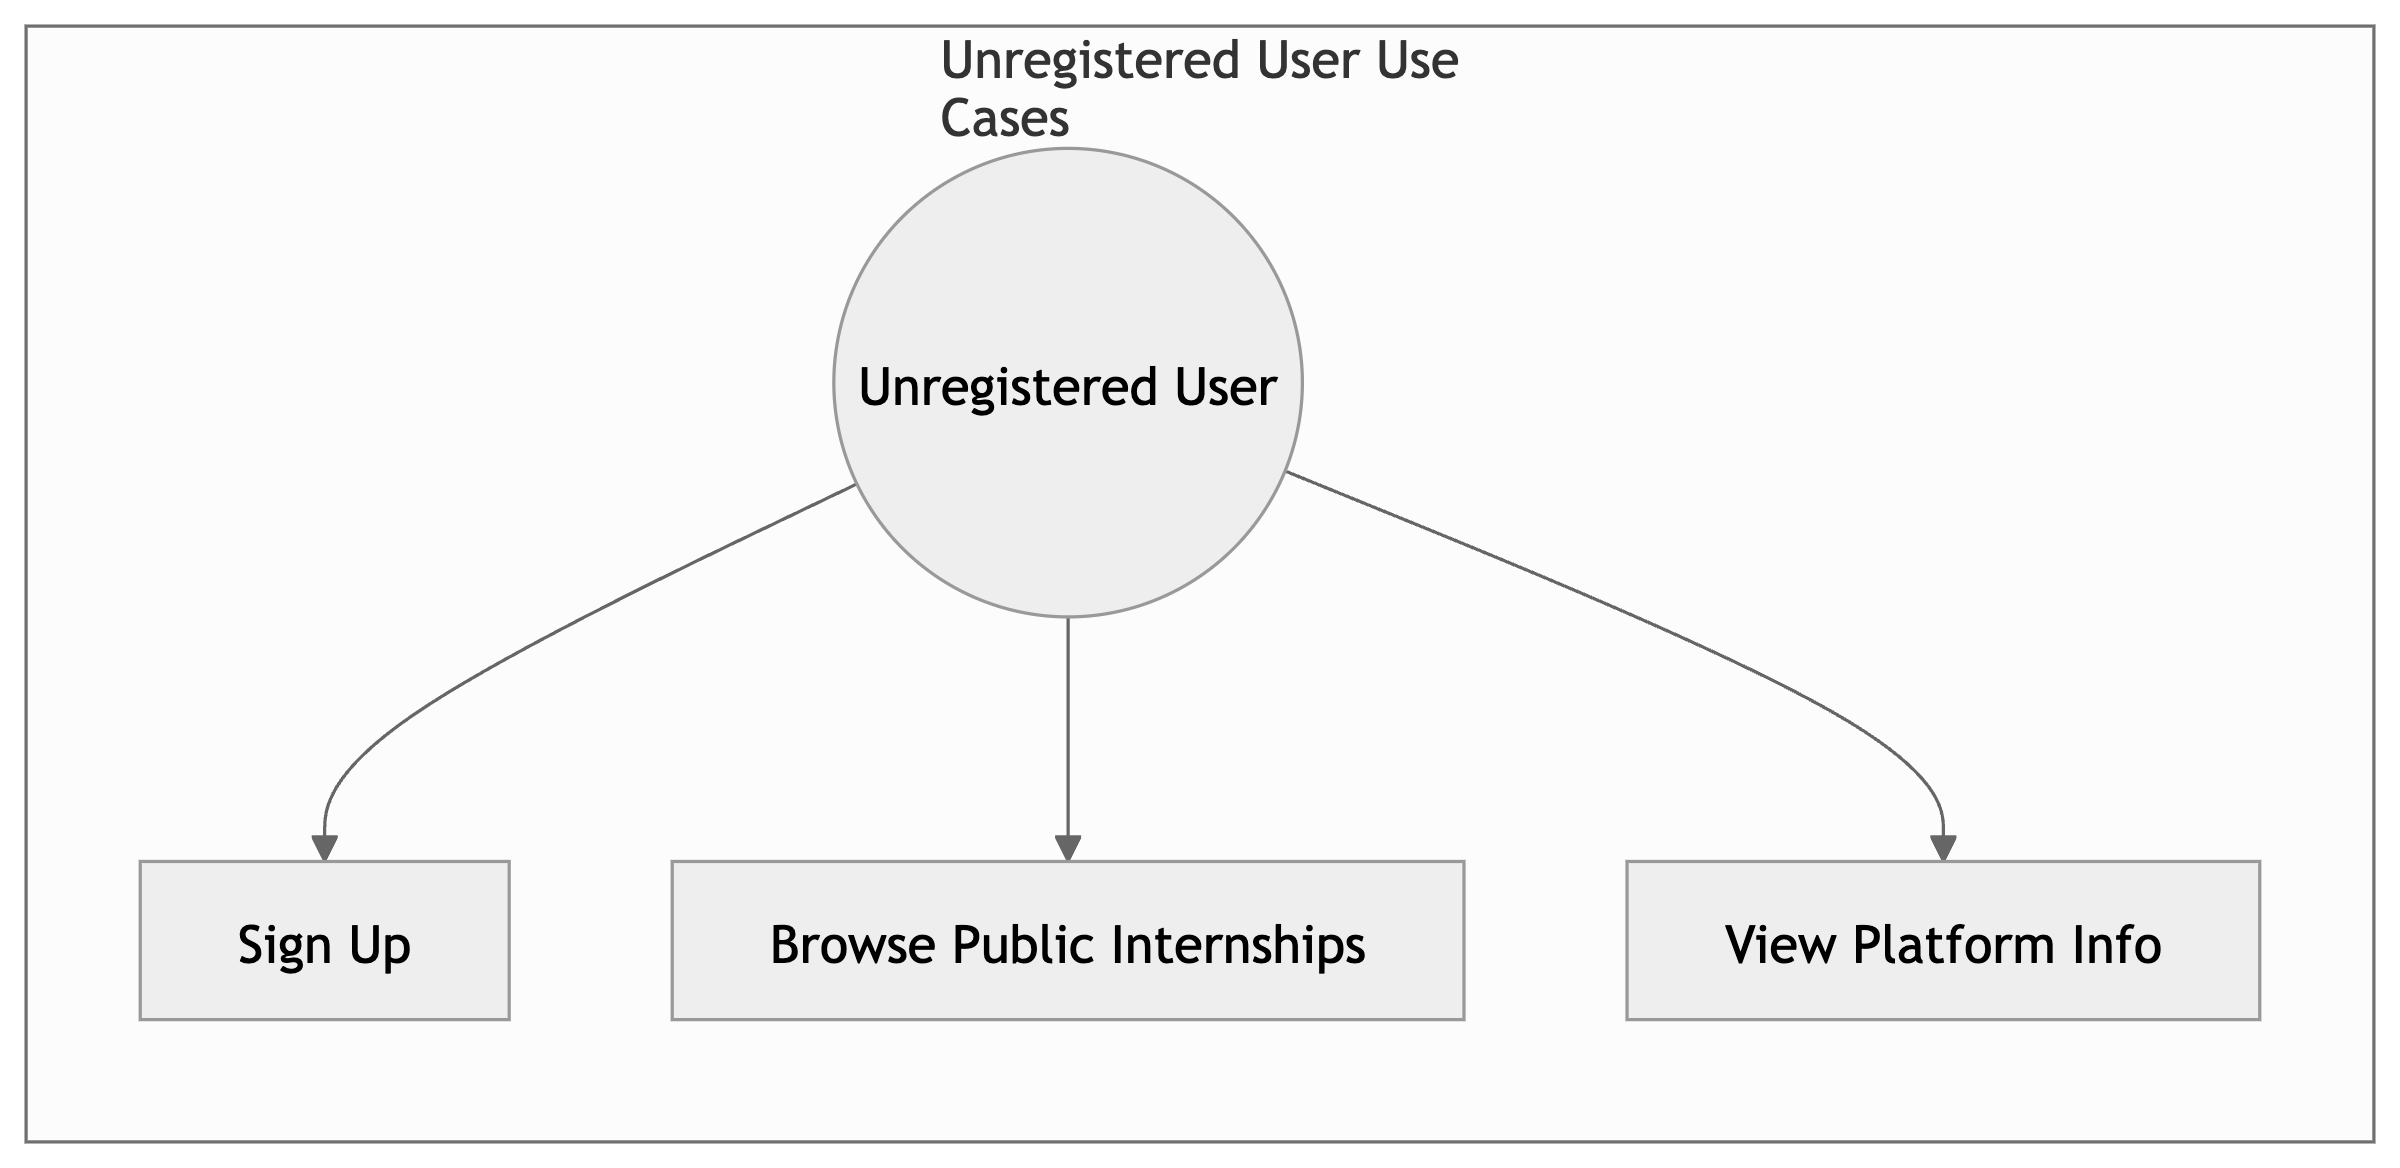
\includegraphics[width=1\linewidth]{JhaBhatiaSharma/Images/Use Case Diagrams/UnregisteredUser.png}
        \caption{Use Cases Diagram for Unregistered Users.} 
        \label{fig:UnregisteredUC}%
    \end{center}
\end{figure}



\begin{figure}[H]
    \begin{center}
        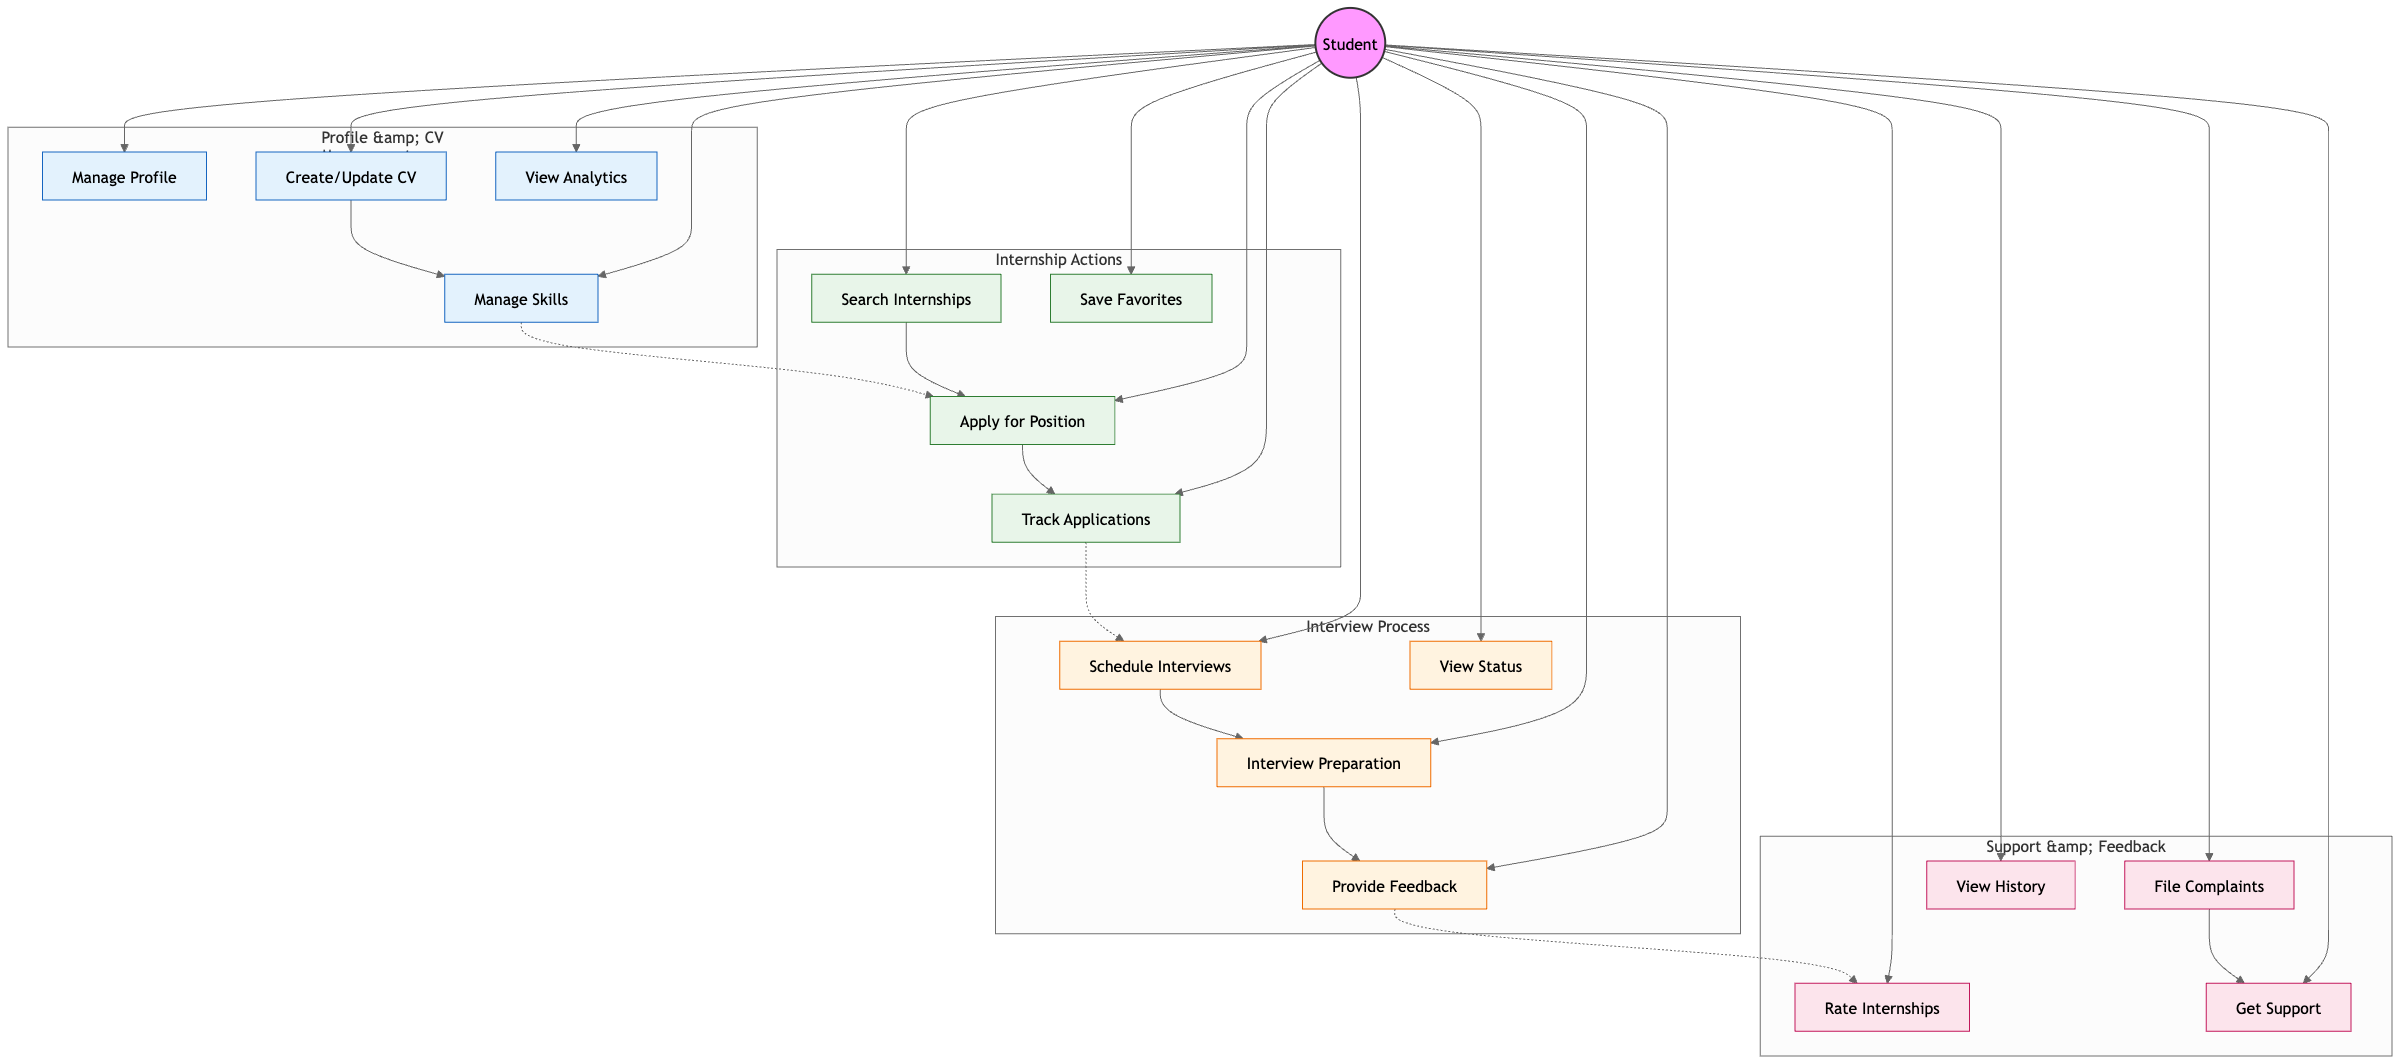
\includegraphics[width=1.15\linewidth]{JhaBhatiaSharma/Images/Use Case Diagrams/Student.png}
        \caption{Use Cases Diagram for Students}
        \label{fig:EducatorUC}%
    \end{center}
\end{figure}



\begin{figure}[H]
    \begin{center}
        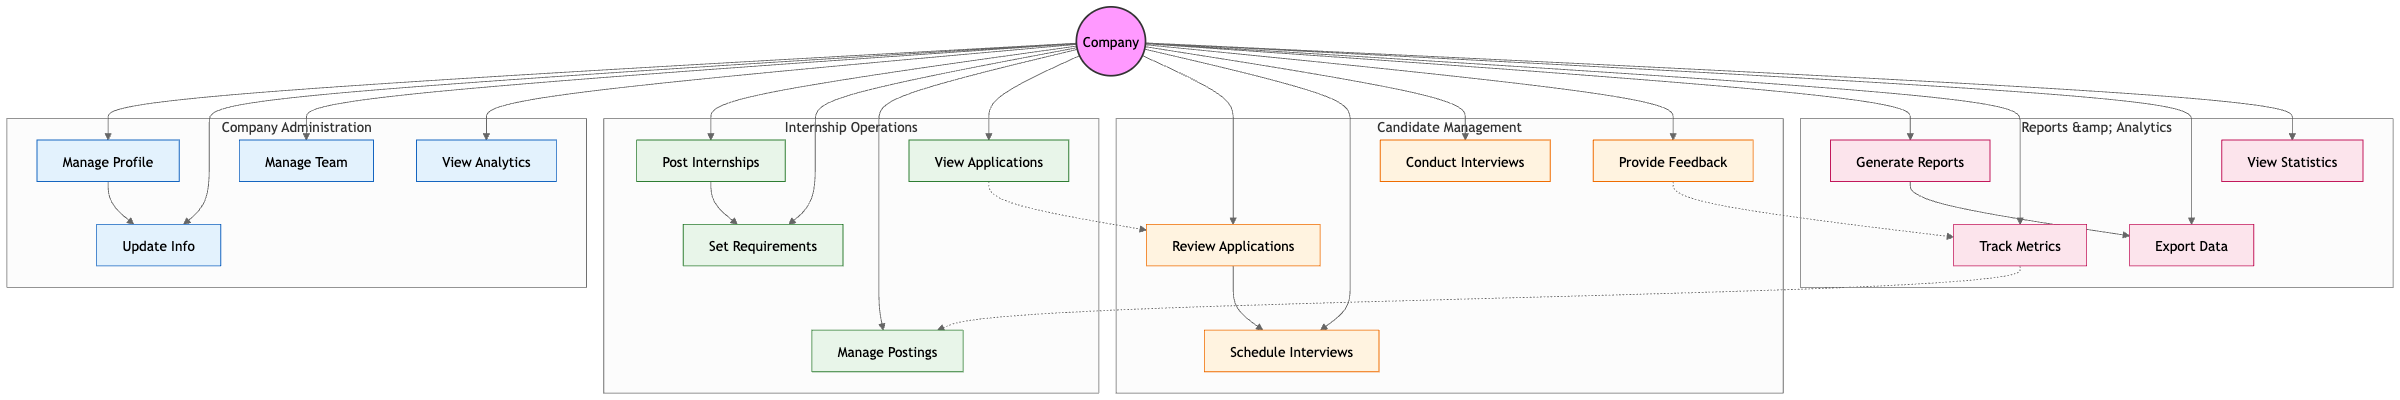
\includegraphics[width=\dimexpr\paperwidth-2cm\relax, height=4cm]{JhaBhatiaSharma/Images/Use Case Diagrams/Company.png}
        \caption{Use Cases Diagram for Companies.}
        \label{fig:CompanyUC}%
    \end{center}
\end{figure}

\begin{figure}[H]
    \begin{center}
        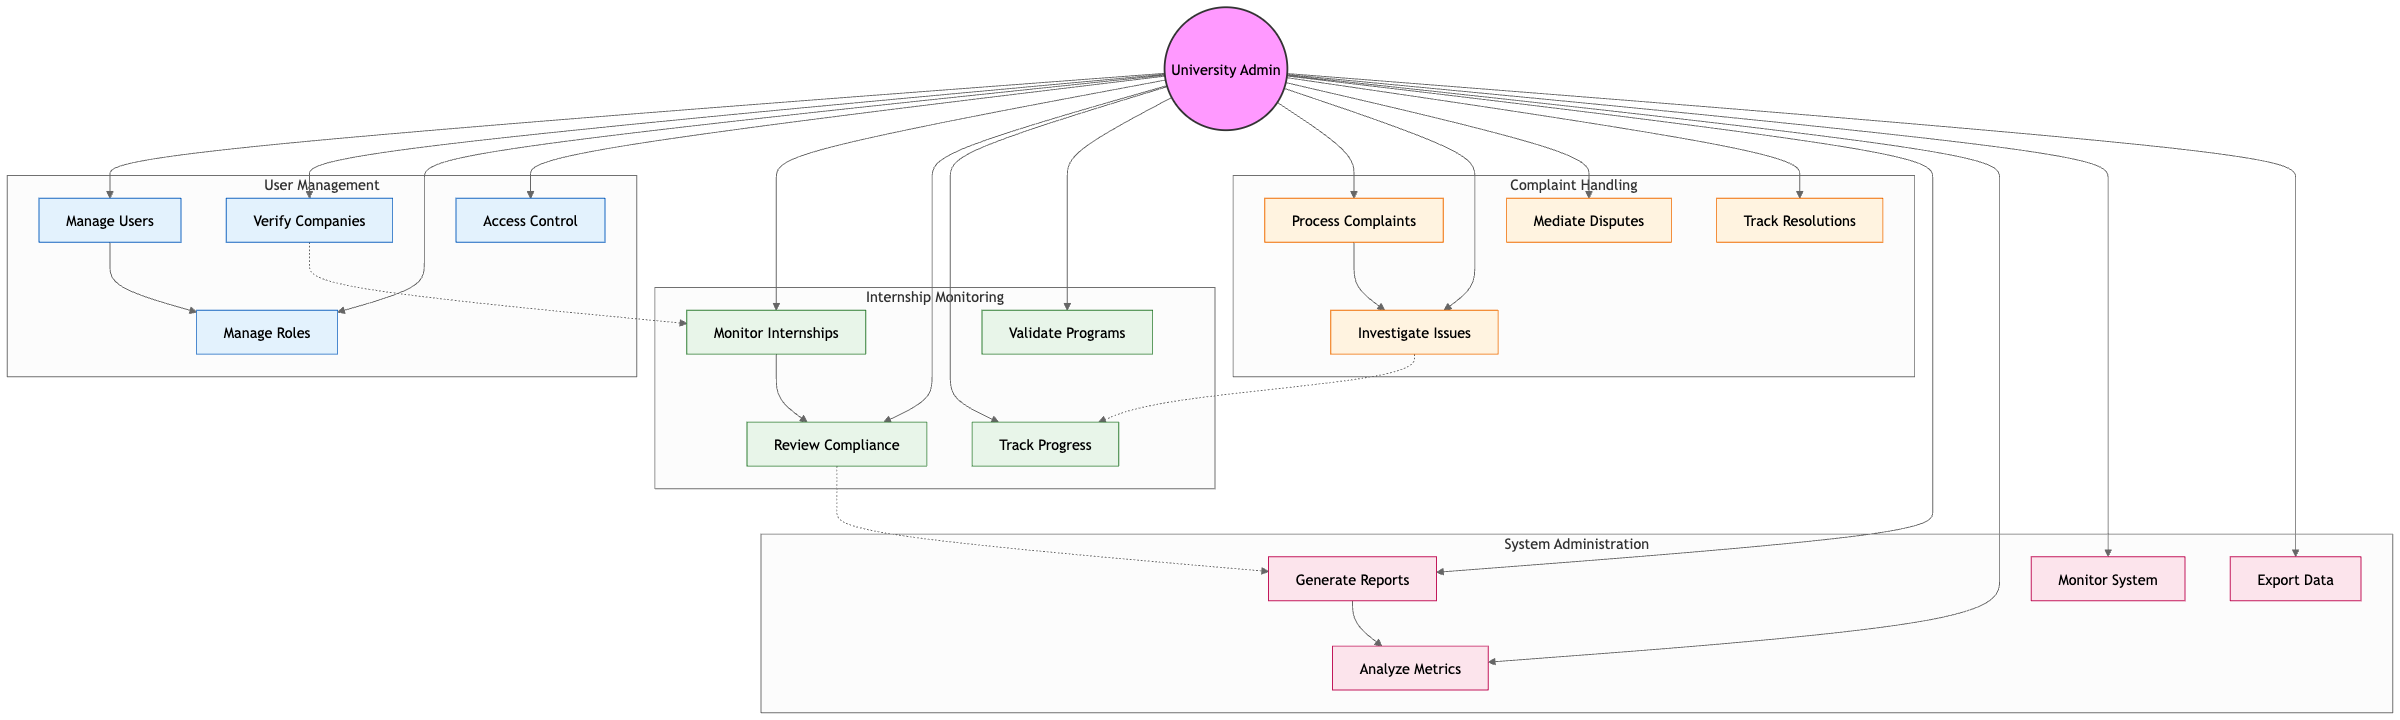
\includegraphics[width=1.1\linewidth, height=4cm]{JhaBhatiaSharma/Images/Use Case Diagrams/Admin.png}
        \caption{Use Cases Diagram for University Admin.}
        \label{fig:AdminUC}%
    \end{center}
\end{figure}

\subsection{Use cases}
\label{subsec: use_cases}%
\newcounter{uc}
\setcounter{uc}{1}
\newcommand{\cuc}{\theuc\stepcounter{uc}}
The primary identified use cases are described and illustrated in this section.
Each of them has a table with \textbf{entry conditions, event row, exit conditions, and exceptions, as well as a sequence diagram} that displays the messages sent back and forth between the called functions and the entities.

\subsubsection*{UC\cuc . Student Registration}
\begin{center}
    \begin{longtable}{|l|p{0.75\linewidth}|}
        \hline
        \textbf{Actor}            & Company Representative, Email Provider \\
        \hline
        \textbf{Entry Conditions} & 
        \begin{itemize}
            \item Company not registered in S\&C
            \item Representative has company email domain
            \item Company meets platform requirements
        \end{itemize} \\
        \hline
        \textbf{Event Flow}       & 
        \begin{enumerate}
            \item S\&C shows the login form with registration option
            \item Representative clicks on "Create Account"
            \item S\&C displays registration form
            \item Representative selects "Register as Company"
            \item Representative enters initial information:
            \begin{itemize}
                \item Company Name
                \item Company Website
                \item Industry Type
                \item Company Size
                \item Company Email Domain
                \item Representative Name
                \item Representative Position
                \item Password
            \end{itemize}
            \item S\&C validates company information
            \item S\&C performs preliminary company verification:
            \begin{itemize}
                \item Website domain matches email domain
                \item Company exists in business registry (if applicable)
            \end{itemize}
            \item S\&C sends verification email
            \item Representative clicks verification link
            \item S\&C prompts for detailed company information:
            \begin{itemize}
                \item Company Description
                \item Office Locations
                \item Logo Upload
                \item Required Documents
            \end{itemize}
            \item S\&C sends information for admin verification
            \item Admin reviews and approves company
            \item S\&C activates company account
            \item S\&C guides through internship posting process
        \end{enumerate} \\
        \hline
        \textbf{Exit Conditions}   & 
        \begin{itemize}
            \item Company account is created and verified
            \item Company profile is complete
            \item Company can post internships
        \end{itemize} \\
        \hline
        \textbf{Exceptions}       & 
        \begin{enumerate}
            \item \textbf{Company already registered:}
            \begin{itemize}
                \item Show existing company message
                \item Provide contact for account recovery
            \end{itemize}
            \item \textbf{Invalid company email domain:}
            \begin{itemize}
                \item Request valid company email
                \item Provide business verification alternatives
            \end{itemize}
            \item \textbf{Company verification failed:}
            \begin{itemize}
                \item Request additional verification documents
                \item Provide support contact
            \end{itemize}
            \item \textbf{Admin rejection:}
            \begin{itemize}
                \item Notify reason for rejection
                \item Provide appeal process information
            \end{itemize}
            \item \textbf{Incomplete required documents:}
            \begin{itemize}
                \item List missing documents
                \item Save partial progress
                \item Allow later completion
            \end{itemize}
        \end{enumerate} \\
        \hline
        \caption{Student Registration Use Case.}
        \label{tab:student_registration_use_case}
    \end{longtable}
\end{center}

\begin{figure}[H]
    \begin{center}
        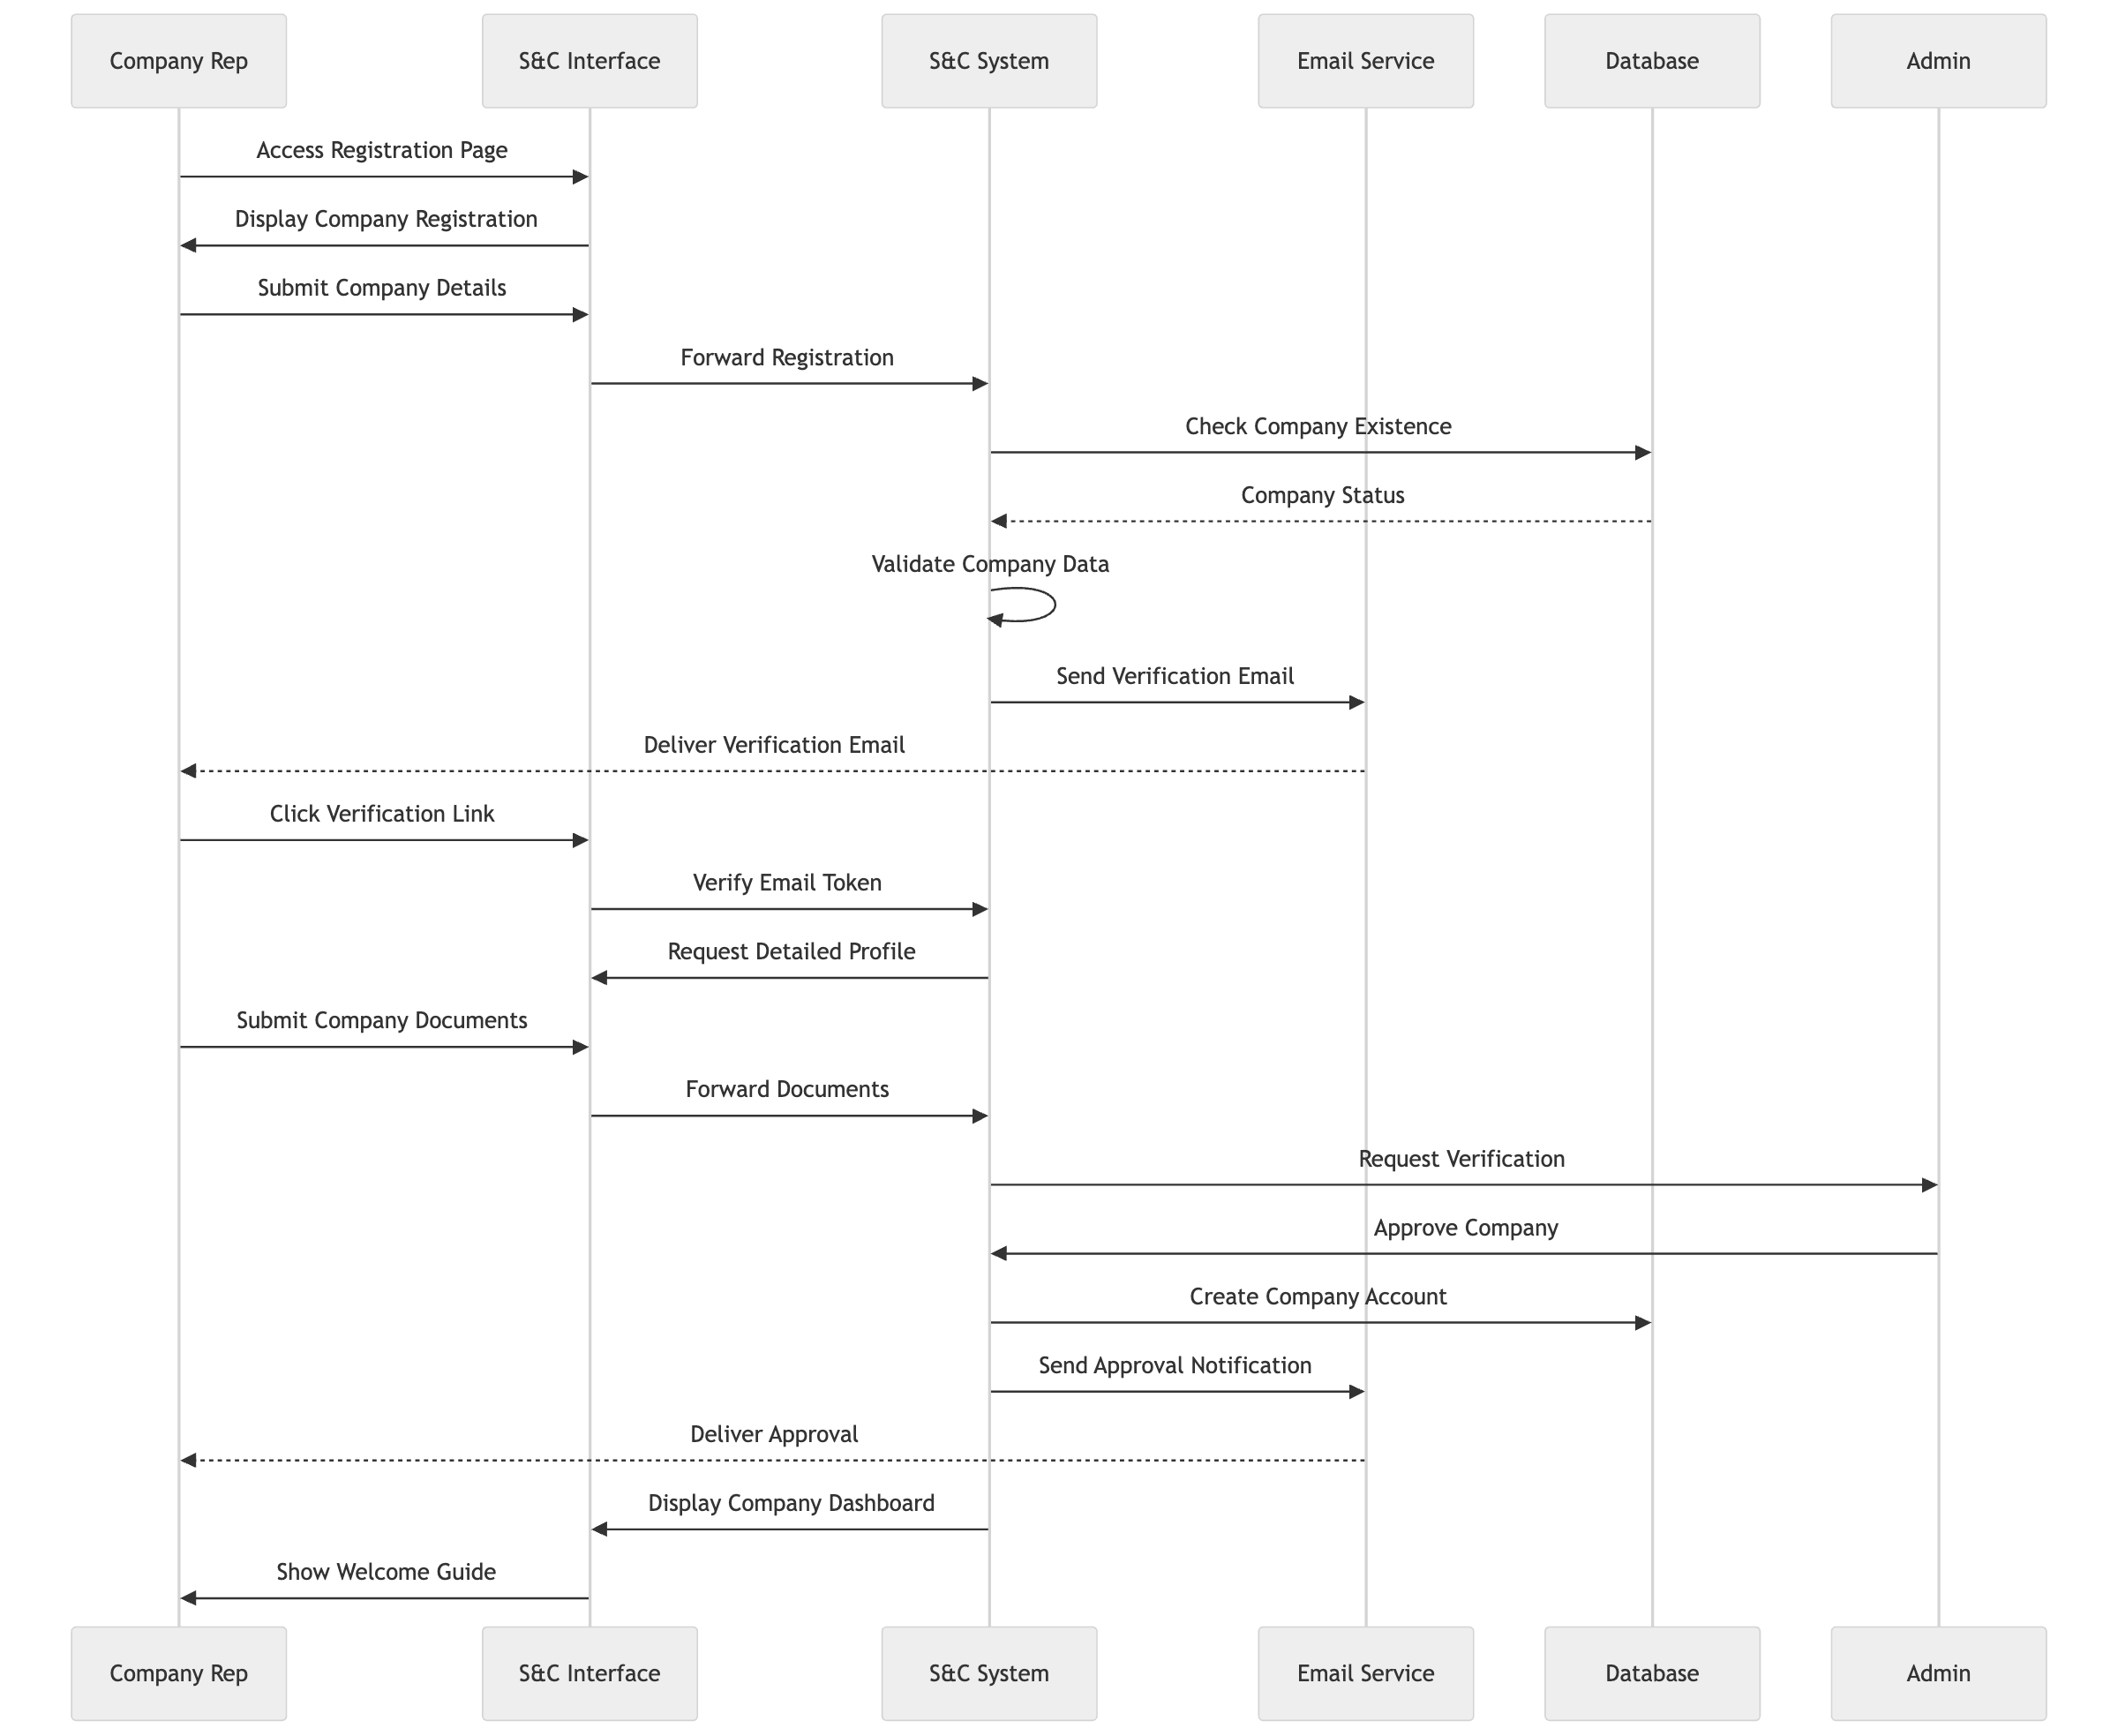
\includegraphics[width=1.15\linewidth, height=\paperheight, keepaspectratio=true]{JhaBhatiaSharma/Images/Sequence Diagrams/StudentRegistration.png}
        \caption{Sequence Diagram for Student Registration}
        \label{fig:signup_as_ED_seqd}%
    \end{center}
\end{figure}

\subsubsection*{UC\cuc . Company Registration}
\begin{center}
    \begin{longtable}{|l|p{0.75\linewidth}|}
        \hline
        \textbf{Actor}            & Company Representative, Email Provider \\
        \hline
        \textbf{Entry Conditions} & 
        \begin{itemize}
            \item Company not registered in S\&C
            \item Representative has company email domain
            \item Company meets platform requirements
        \end{itemize} \\
        \hline
        \textbf{Event Flow}       & 
        \begin{enumerate}
            \item S\&C shows the login form with registration option.
            \item Representative clicks on "Create Account".
            \item S\&C displays registration form.
            \item Representative selects "Register as Company".
            \item Representative enters initial information:
            \begin{itemize}
                \item Company Name
                \item Company Website
                \item Industry Type
                \item Company Size
                \item Company Email Domain
                \item Representative Name
                \item Representative Position
                \item Password
            \end{itemize}
            \item S\&C validates company information.
            \item S\&C performs preliminary company verification:
            \begin{itemize}
                \item Website domain matches email domain
                \item Company exists in business registry (if applicable)
            \end{itemize}
            \item S\&C sends verification email.
            \item Representative clicks verification link.
            \item S\&C prompts for detailed company information:
            \begin{itemize}
                \item Company Description
                \item Office Locations
                \item Logo Upload
                \item Required Documents
            \end{itemize}
            \item S\&C sends information for admin verification.
            \item Admin reviews and approves company.
            \item S\&C activates company account.
            \item S\&C guides through internship posting process.
        \end{enumerate} \\
        \hline
        \textbf{Exit Conditions}   & 
        \begin{itemize}
            \item Company account is created and verified.
            \item Company profile is complete.
            \item Company can post internships.
        \end{itemize} \\
        \hline
        \textbf{Exceptions}       & 
        \begin{enumerate}
            \item \textbf{Company already registered:}
            \begin{itemize}
                \item Show existing company message.
                \item Provide contact for account recovery.
            \end{itemize} 
            \item \textbf{Invalid company email domain:} \begin{itemize}
                \item Request valid company email.
                \item Provide business verification alternatives.
            \end{itemize} 
            \item \textbf{Company verification failed:} \begin{itemize}
                \item Request additional verification documents.
                \item Provide support contact.
            \end{itemize} 
            \item \textbf{Admin rejection:} 
            \begin{itemize}
                \item Notify reason for rejection.
                \item Provide appeal process information.
            \end{itemize} 
            \item \textbf{Incomplete required documents:} \begin{itemize}
                \item List missing documents.
                \item Save partial progress.
                \item Allow later completion.
            \end{itemize}  
        \end{enumerate} \\
        \hline
        \caption{Company Registration use case.}
        \label{tab:company_registration_use_case}
    \end{longtable}
\end{center}


\begin{figure}[H]
    \begin{center}
        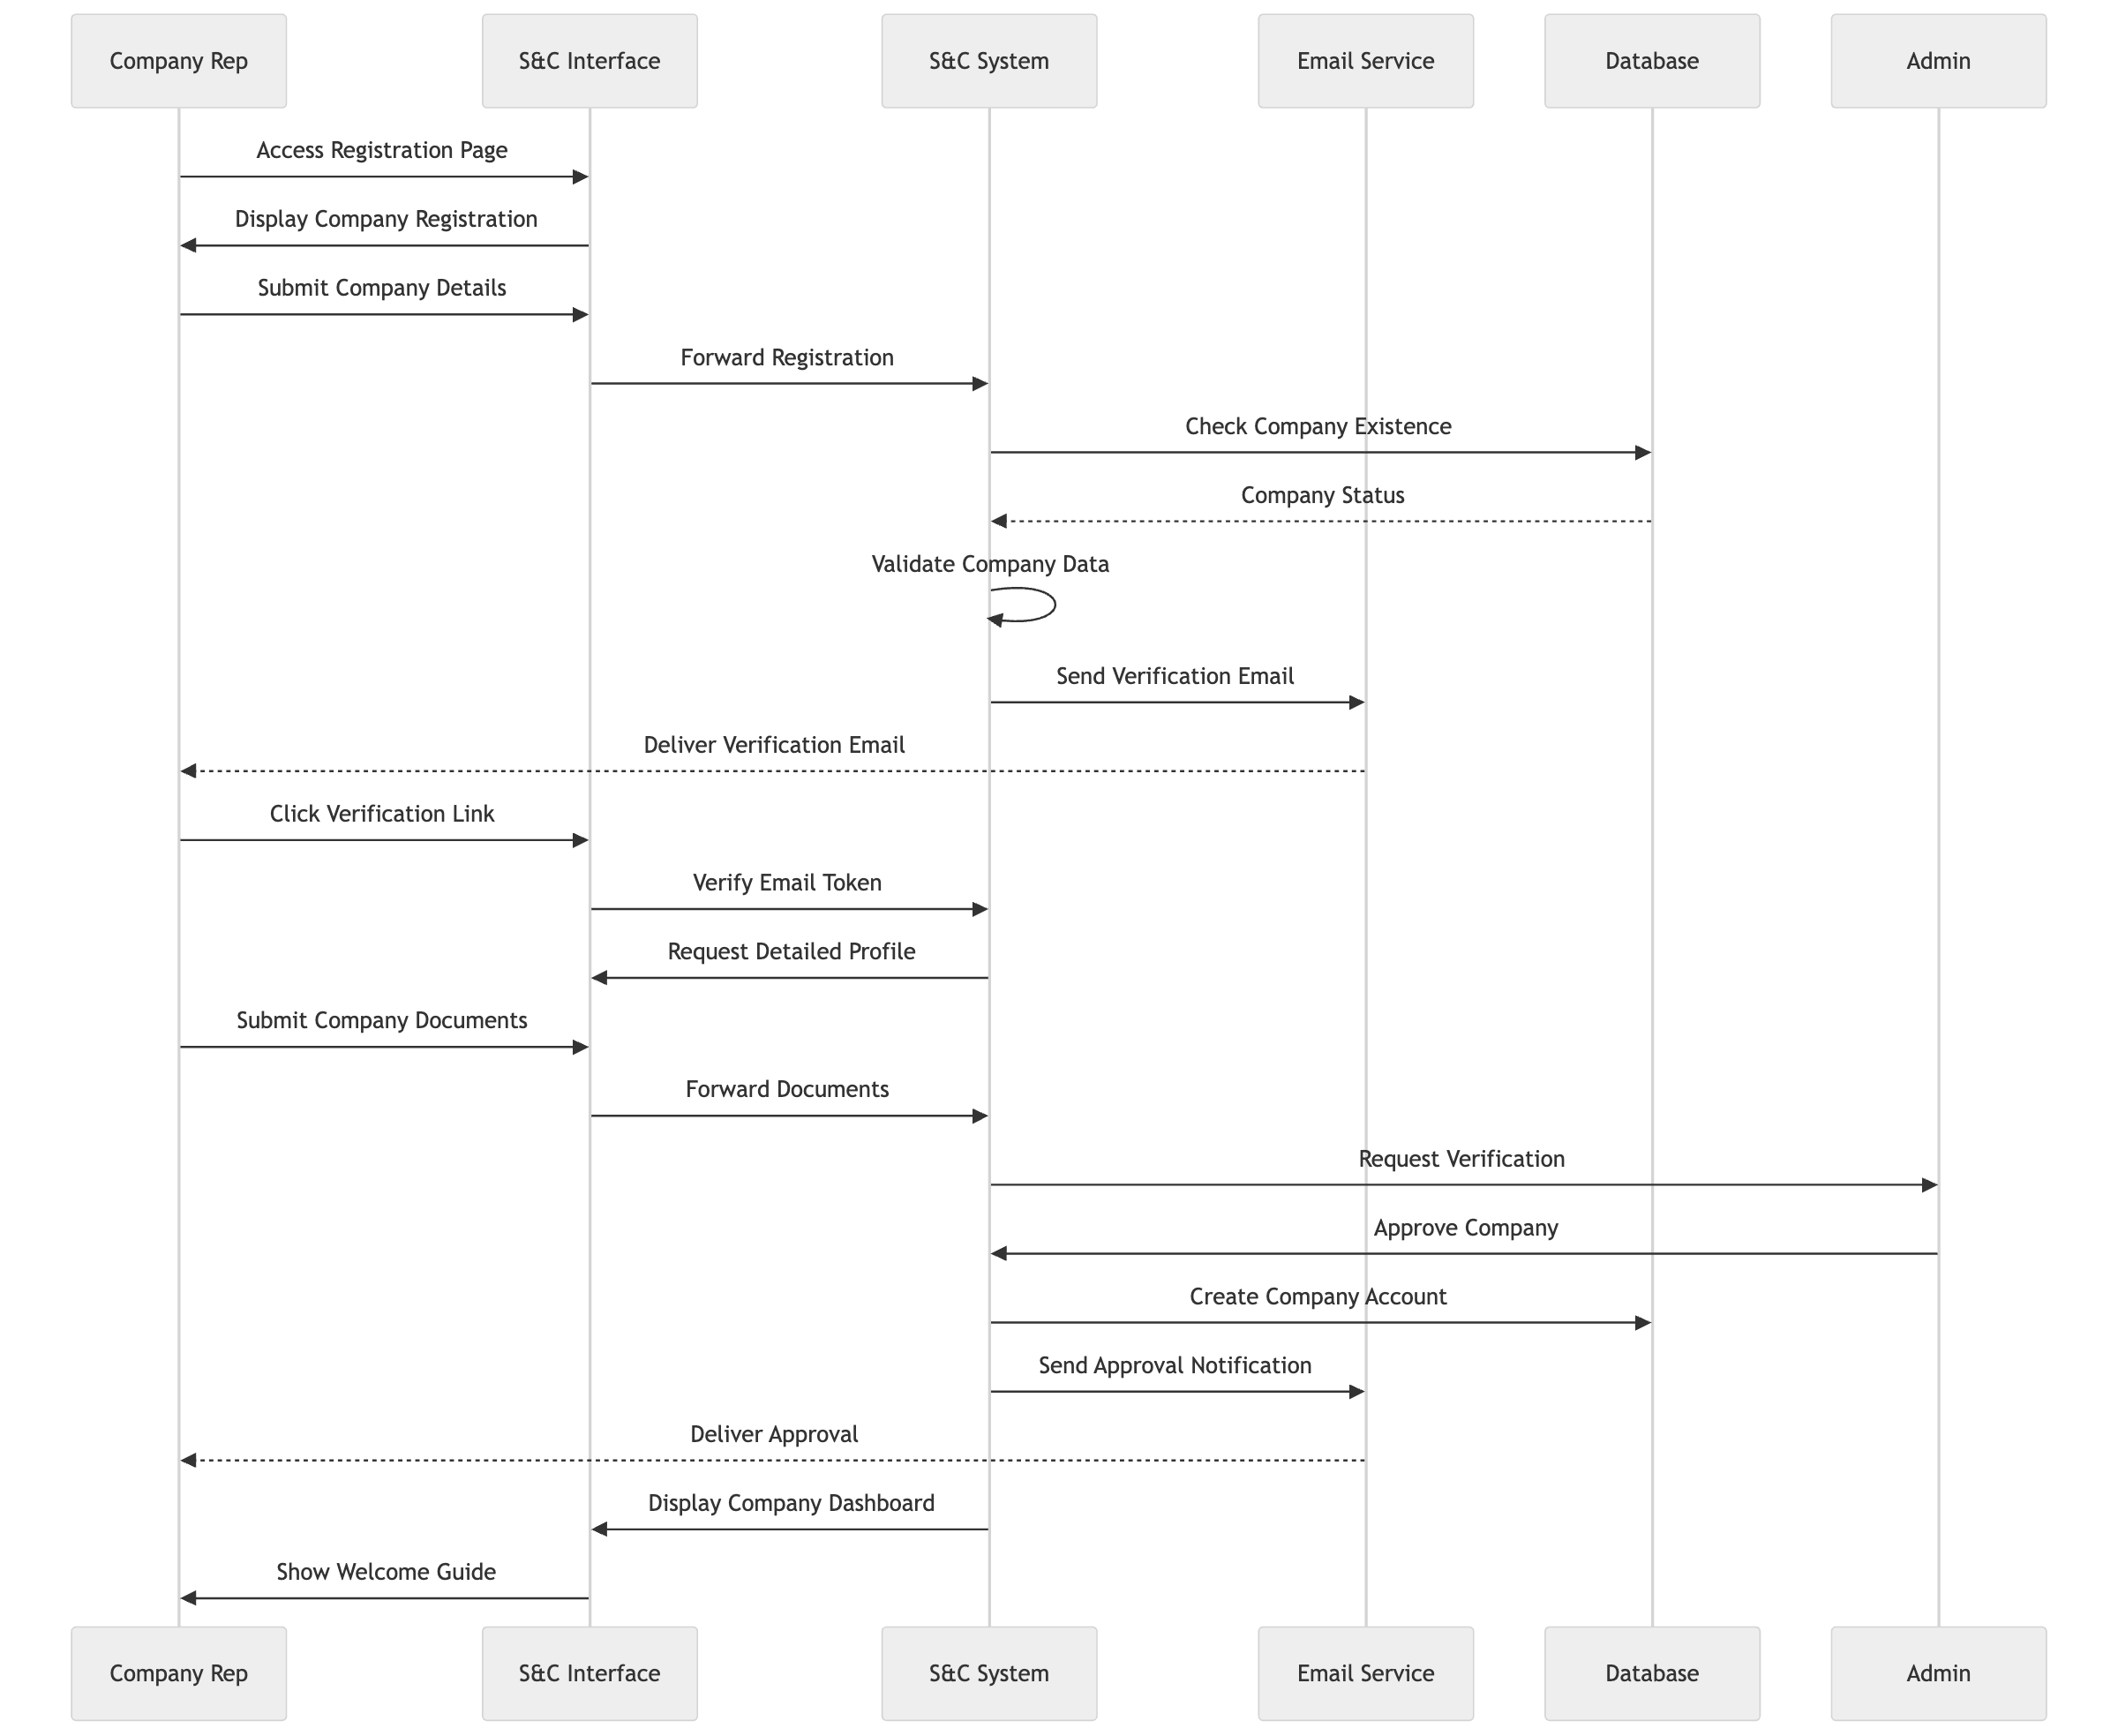
\includegraphics[width=1\linewidth]{JhaBhatiaSharma/Images/Sequence Diagrams/CompanyRegistration.png}
        \caption{Sequence Diagram for Company Registration}
        \label{fig:signup_as_ST_seqd}%
    \end{center}
\end{figure}

\subsubsection*{UC\cuc . Internship Posting}
\begin{center}
    \begin{longtable}{|l|p{0.75\linewidth}|}
        \hline
        \textbf{Actor}            & Company Representative \\
        \hline
        \textbf{Entry Conditions} & 
        \begin{itemize}
            \item Company is verified and logged in
            \item Company profile is complete
            \item Company has posting privileges
        \end{itemize} \\
        \hline
        \textbf{Event Flow}       & 
        \begin{enumerate}
            \item Company accesses internship management dashboard.
            \item Clicks "Post New Internship" button.
            \item S\&C displays internship creation form.
            \item Company enters internship details:
            \begin{itemize}
                \item Position Title
                \item Department
                \item Duration
                \item Start Date
                \item Required Skills
                \item Preferred Skills
                \item Educational Requirements
                \item Responsibilities
                \item Compensation Details
                \item Application Deadline
                \item Number of Positions
                \item Location/Remote Status
            \end{itemize}
            \item Company sets additional preferences:
            \begin{itemize}
                \item Interview Process Steps
                \item Required Documents
                \item Assessment Criteria
            \end{itemize}
            \item S\&C validates all input fields.
            \item Company previews posting.
            \item Company submits for review.
            \item S\&C performs automated checks:
            \begin{itemize}
                \item Content appropriateness
                \item Completeness
                \item Compliance with platform rules
            \end{itemize}
            \item S\&C processes posting:
            \begin{itemize}
                \item Indexes for search
                \item Matches with student profiles
                \item Generates recommendations
            \end{itemize}
            \item S\&C activates posting.
            \item Notifies matching students.
        \end{enumerate} \\
        \hline
        \textbf{Exit Conditions}   & 
        \begin{itemize}
            \item Internship is posted and visible
            \item Matching students are notified
            \item Position appears in search results
        \end{itemize} \\
        \hline
        \textbf{Exceptions}       & 
        \begin{enumerate}
            \item \textbf{Incomplete Required Fields:} \begin{itemize}
                \item Highlight missing fields.
                \item Save as draft.
            \end{itemize} 
            \item \textbf{Invalid Date Combinations:} 
            \begin{itemize}
                \item Show date validation error.
                \item Suggest valid date ranges.
            \end{itemize} 
            \item \textbf{Non-Compliant Content:} 
            \begin{itemize}
                \item Flag specific issues.
                \item Provide compliance guidelines.
            \end{itemize} 
            \item \textbf{Duplicate Posting:} 
            \begin{itemize}
                \item Show existing posting.
                \item Offer update option.
            \end{itemize} 
            \item \textbf{Posting Limit Reached:} 
            \begin{itemize}
                \item Show upgrade options.
                \item Manage existing posts.
            \end{itemize} 
        \end{enumerate} \\
        \hline
        \caption{Internship Posting Use Case.}
        \label{tab:internship_posting_use_case}
    \end{longtable}
\end{center}

\begin{figure}[H]
    \begin{center}
        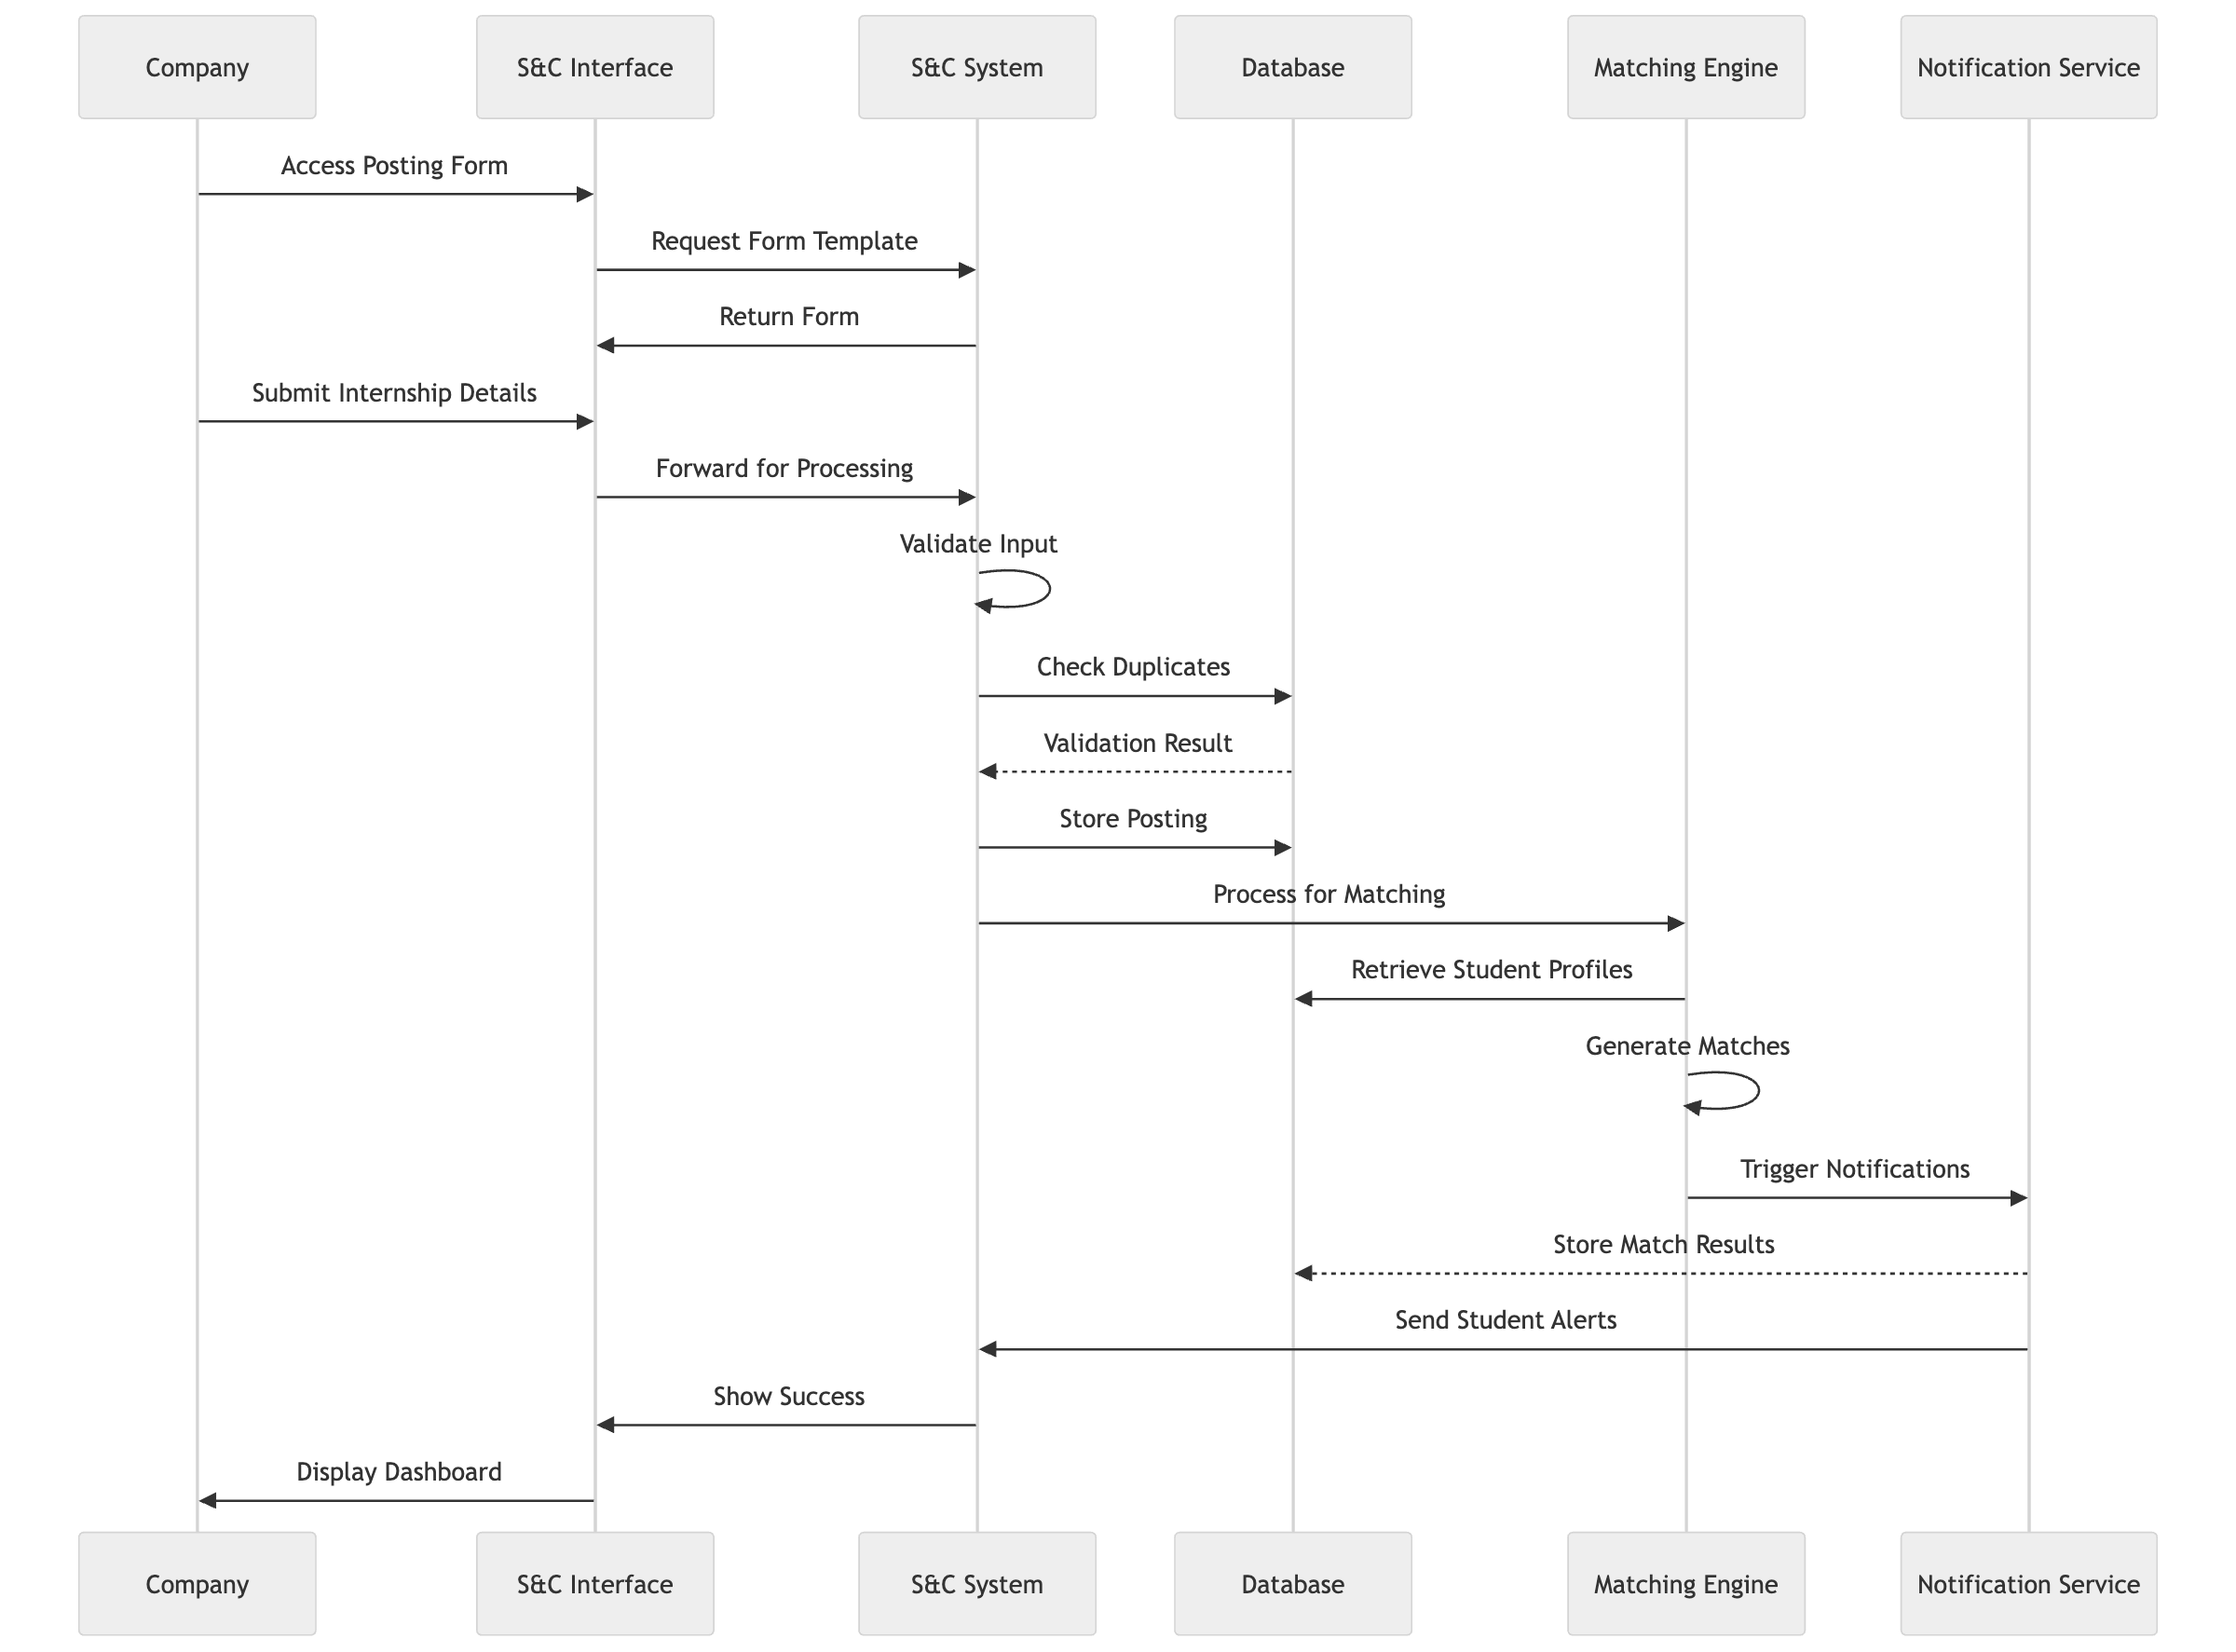
\includegraphics[width=1\linewidth]{JhaBhatiaSharma/Images/Sequence Diagrams/InternshipPosting.png}
        \caption{Sequence Diagram for Internship Posting}
        \label{fig:InternPost}%
    \end{center}
\end{figure}

\subsubsection*{UC\cuc . Student Application Process}
\begin{center}
    \begin{longtable}{|l|p{0.75\linewidth}|}
        \hline
        \textbf{Actor}            & Student \\
        \hline
        \textbf{Entry Conditions} & 
        \begin{itemize}
            \item Student is logged in
            \item Profile and CV are complete
            \item Meets basic internship requirements
        \end{itemize} \\
        \hline
        \textbf{Event Flow}       & 
        \begin{enumerate}
            \item Student finds internship through:
            \begin{itemize}
                \item Direct search
                \item Recommendations
                \item Email notification
            \end{itemize}
            \item Student reviews internship details:
            \begin{itemize}
                \item Company information
                \item Position requirements
                \item Terms and conditions
            \end{itemize}
            \item Student initiates application:
            \begin{itemize}
                \item Selects CV version
                \item Customizes cover letter
                \item Answers screening questions
                \item Provides additional documents
            \end{itemize}
            \item S\&C performs preliminary checks:
            \begin{itemize}
                \item Eligibility verification
                \item Previous applications
                \item Document completeness
            \end{itemize}
            \item Student reviews application package.
            \item Student submits application.
            \item S\&C processes application:
            \begin{itemize}
                \item Updates application counter
                \item Indexes for company search
                \item Generates application ID
            \end{itemize}
            \item Company receives notification.
            \item S\&C updates student dashboard.
            \item Application tracking begins.
        \end{enumerate} \\
        \hline
        \textbf{Exit Conditions}   & 
        \begin{itemize}
            \item Application is submitted
            \item Company is notified
            \item Student can track status
        \end{itemize} \\
        \hline
        \textbf{Exceptions}       & 
        \begin{enumerate}
            \item \textbf{Incomplete Profile:} 
            \begin{itemize}
                \item Redirect to profile completion.
                \item Save application draft.
            \end{itemize} 
            \item \textbf{Missing Required Documents:} \begin{itemize}
                \item List required documents.
                \item Provide upload options.
            \end{itemize} 
            \item \textbf{Previous Application Exists:} \begin{itemize}
                \item Show existing application.
                \item Offer update option.
            \end{itemize} 
            \item \textbf{Deadline Passed:} 
            \begin{itemize}
                \item Show expired notice.
                \item Suggest similar positions.
            \end{itemize} 
            \item \textbf{Requirements Not Met:} 
            \begin{itemize}
                \item Show specific gaps.
                \item Suggest skill development.
            \end{itemize} 
        \end{enumerate} \\
        \hline
        \caption{Student Application Process Use Case.}
        \label{tab:student_application_process_use_case}
    \end{longtable}
\end{center}


\begin{figure}[H]
    \begin{center}
        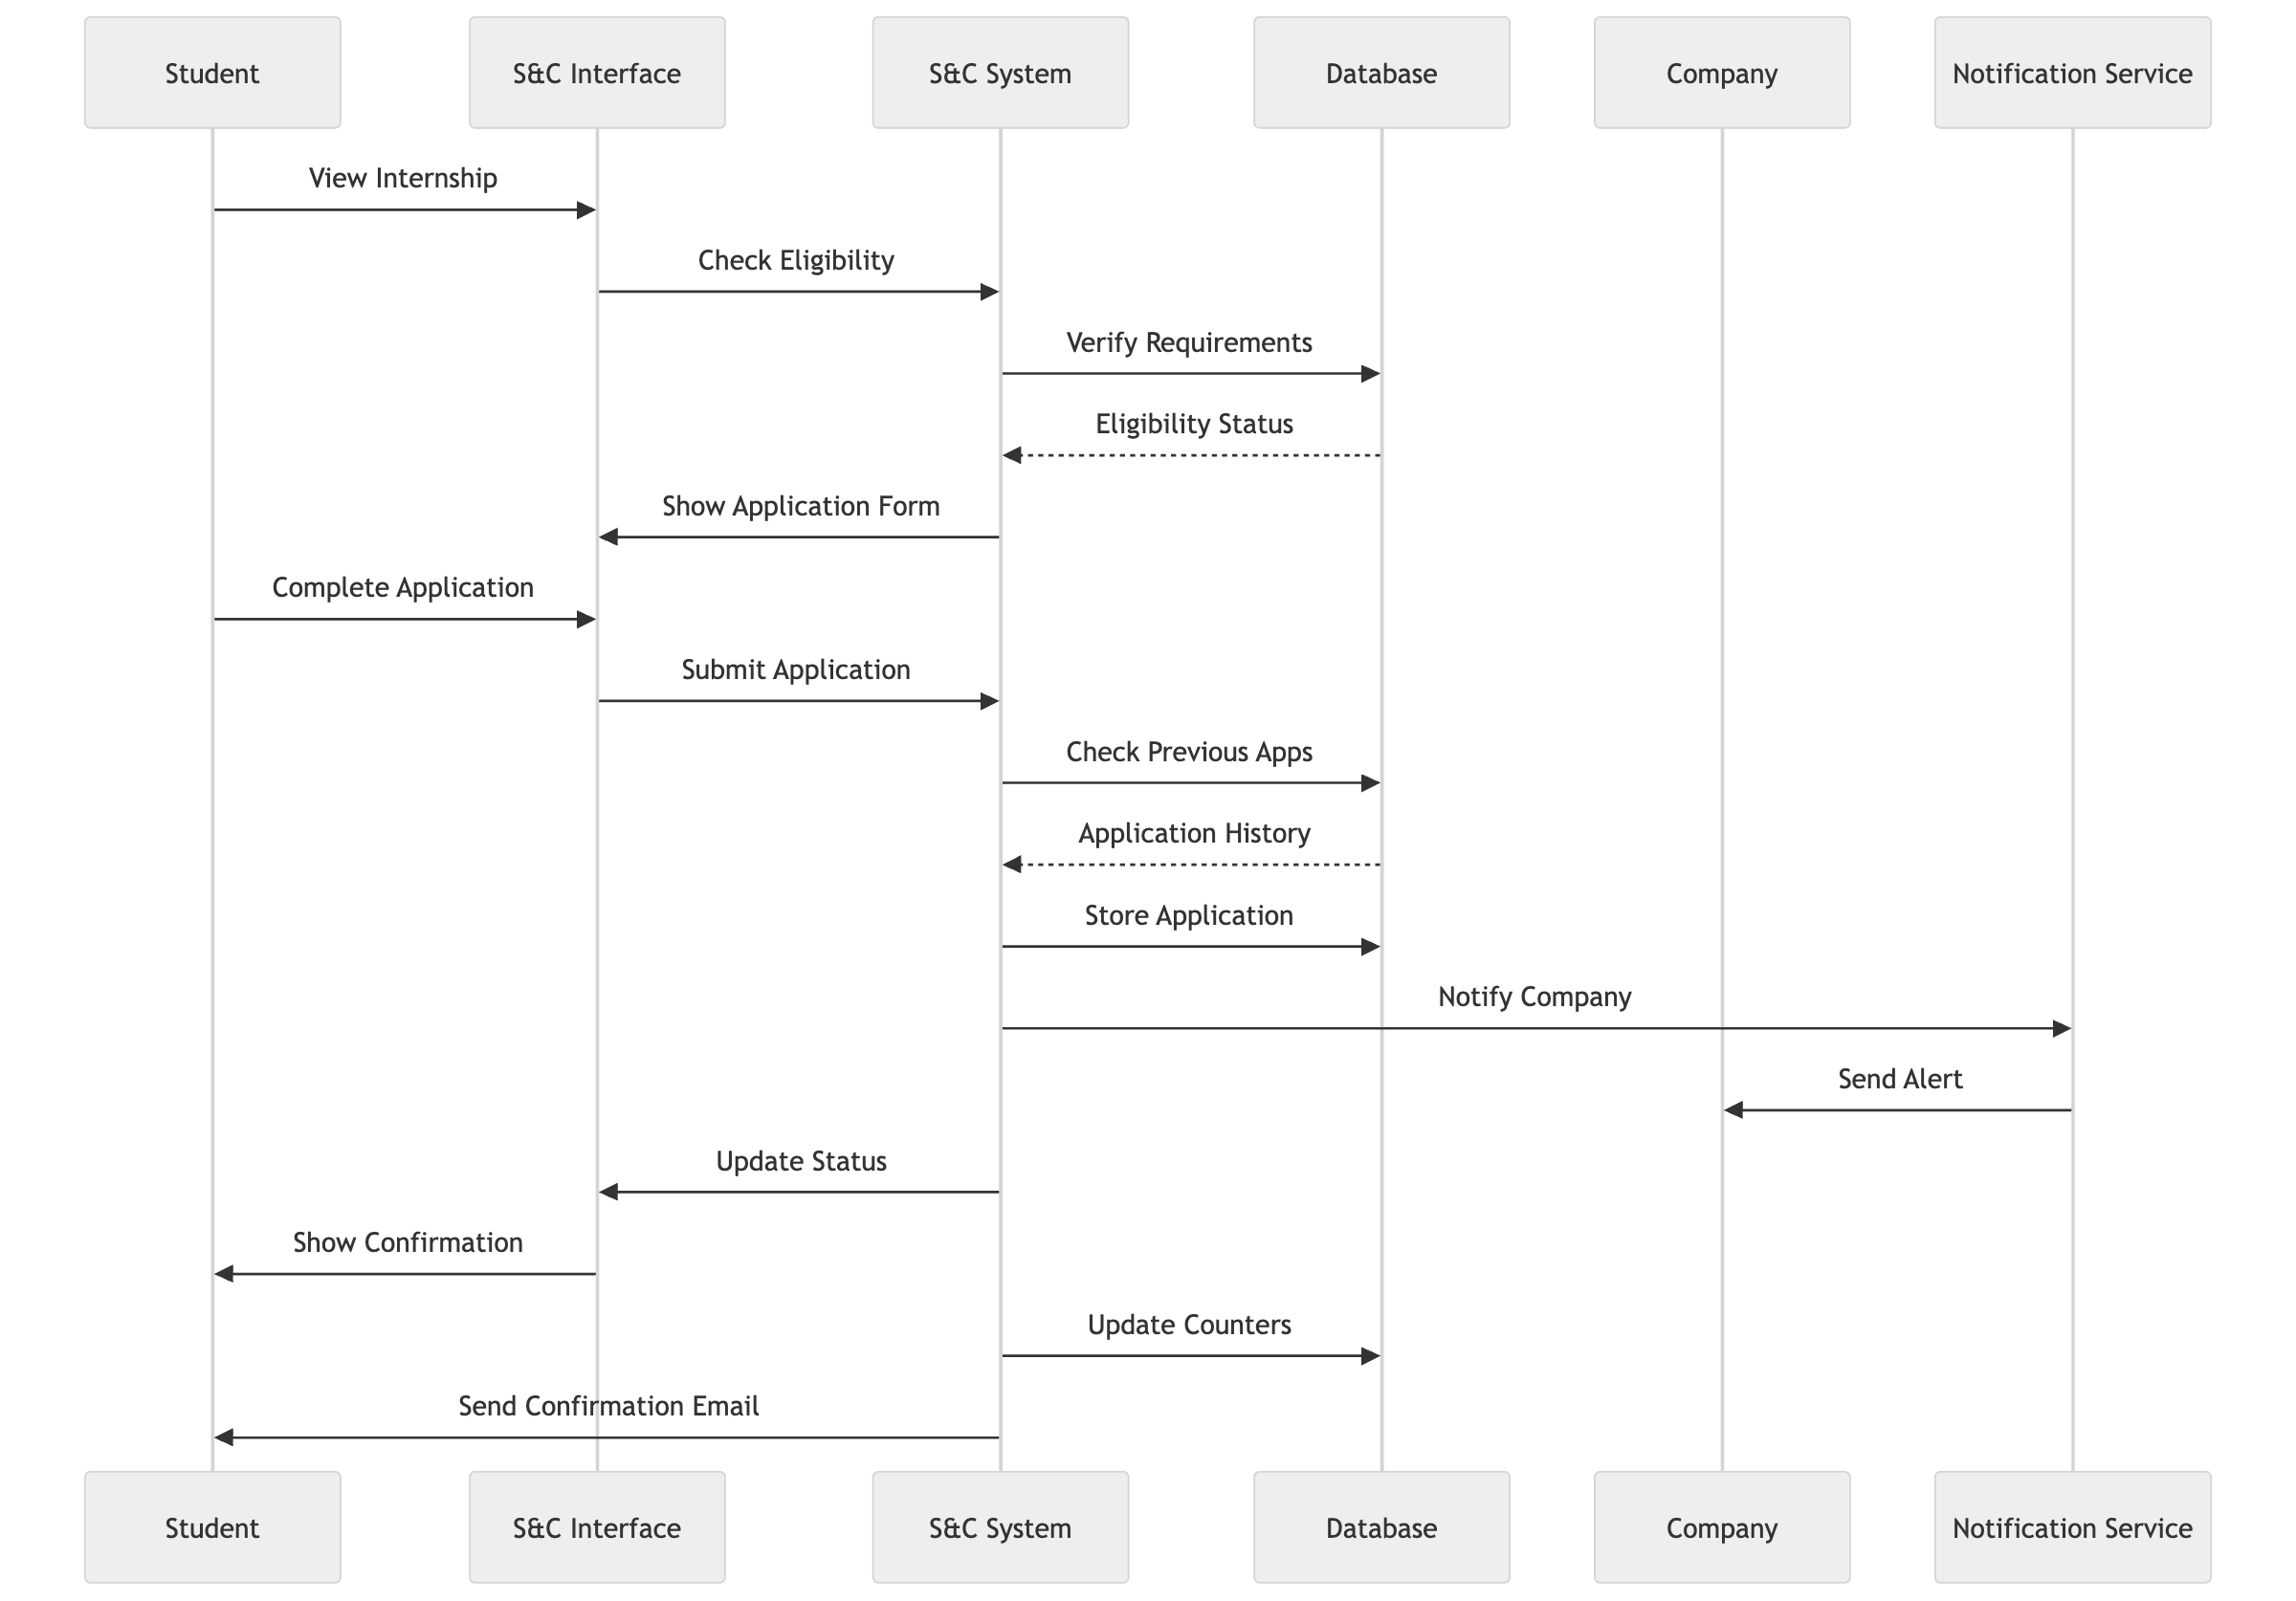
\includegraphics[width=1\linewidth]{JhaBhatiaSharma/Images/Sequence Diagrams/StudentApplication.png}
        \caption{Sequence Diagram for Student Application Process}
        \label{fig:create_a_Tournament_seqd}%
    \end{center}
\end{figure}

\subsubsection*{UC\cuc . Interview Management}
\begin{center}
    \begin{longtable}{|l|p{0.75\linewidth}|}
        \hline
        \textbf{Actor}            & Company Representative, Student \\
        \hline
        \textbf{Entry Conditions} & 
        \begin{itemize}
            \item Application is shortlisted
            \item Both parties are active users
            \item Interview stage is initiated
        \end{itemize} \\
        \hline
        \textbf{Event Flow}       & 
        \begin{enumerate}
            \item Company reviews application.
            \item Company initiates interview process:
            \begin{itemize}
                \item Selects interview type
                \item Proposes time slots
                \item Sets interview format
            \end{itemize}
            \item S\&C sends interview request to student.
            \item Student receives notification:
            \begin{itemize}
                \item Views proposed slots
                \item Checks interview details
                \item Reviews preparations
            \end{itemize}
            \item Student responds:
            \begin{itemize}
                \item Accepts time slot or
                \item Proposes alternatives
            \end{itemize}
            \item S\&C coordinates scheduling:
            \begin{itemize}
                \item Confirms final time
                \item Sends calendar invites
                \item Provides meeting links
            \end{itemize}
            \item Both parties prepare:
            \begin{itemize}
                \item Access interview materials
                \item Review guidelines
                \item Check technical setup
            \end{itemize}
            \item Interview conducted.
            \item Company provides feedback:
            \begin{itemize}
                \item Evaluation form
                \item Notes and ratings
                \item Decision input
            \end{itemize}
            \item S\&C processes results:
            \begin{itemize}
                \item Updates application status
                \item Notifies student
                \item Records outcomes
            \end{itemize}
        \end{enumerate} \\
        \hline
        \textbf{Exit Conditions}   & 
        \begin{itemize}
            \item Interview is completed
            \item Feedback is recorded
            \item Next steps are initiated
        \end{itemize} \\
        \hline
        \textbf{Exceptions}       & 
        \begin{enumerate}
            \item \textbf{Schedule Conflicts:}
            \begin{itemize}
                \item Rescheduling process
                \item Alternative slot suggestions
            \end{itemize}
            \item \textbf{Technical Issues:}
            \begin{itemize}
                \item Backup contact methods
                \item Rescheduling options
            \end{itemize}
            \item \textbf{No-Show Scenarios:}
            \begin{itemize}
                \item Record incident
                \item Reschedule policy
            \end{itemize}
            \item \textbf{Cancellation Requests:}
            \begin{itemize}
                \item Process cancellation
                \item Update status
            \end{itemize}
            \item \textbf{Feedback Deadline Missed:}
            \begin{itemize}
                \item Send reminders
                \item Escalation process
            \end{itemize}
        \end{enumerate} \\
        \hline
        \caption{Interview Management Use Case.}
        \label{tab:interview_management_use_case}
    \end{longtable}
\end{center}


\begin{figure}[H]
    \begin{center}
        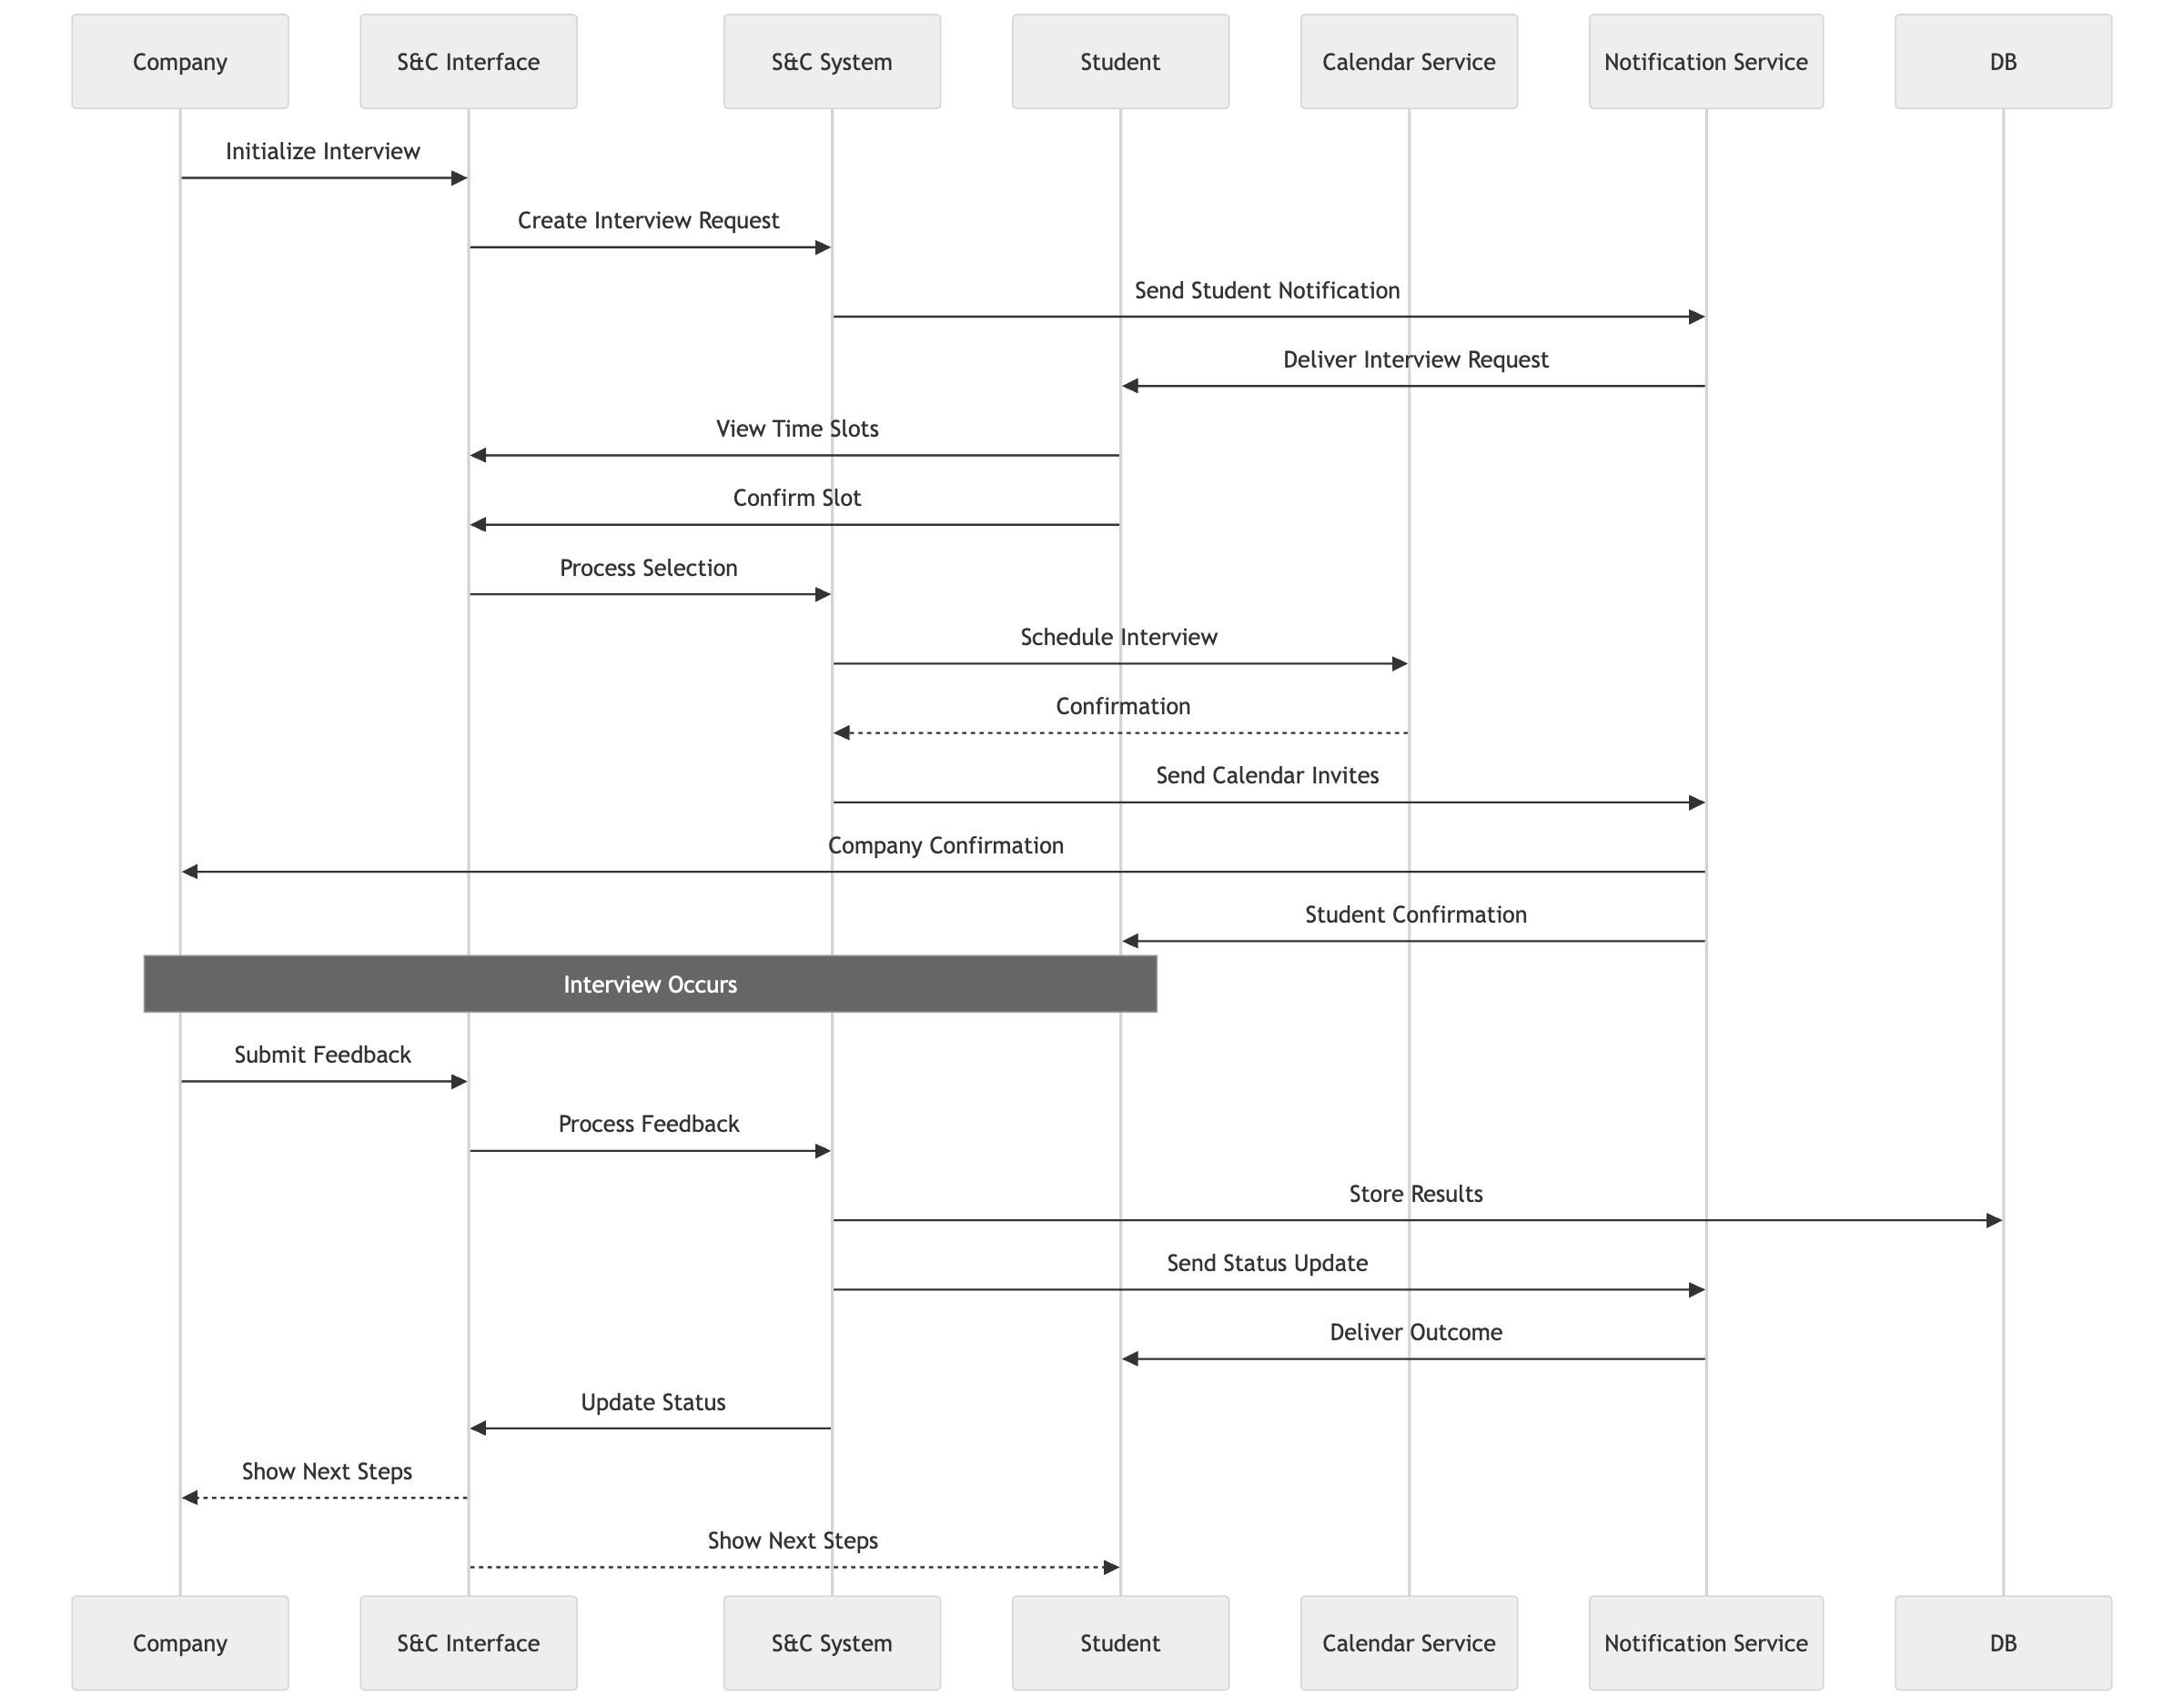
\includegraphics[width=1\linewidth]{JhaBhatiaSharma/Images/Sequence Diagrams/InterviewManagement.png}
        \caption{Sequence Diagram for Interview Management}
        \label{fig:join_a_Tournament_seqd}%
    \end{center}
\end{figure}

\subsubsection*{UC\cuc . Complaint Handling}
\begin{center}
    \begin{longtable}{|l|p{0.75\linewidth}|}
        \hline
        \textbf{Actor}            & Student/Company, University Administrator \\
        \hline
        \textbf{Entry Conditions} & 
        \begin{itemize}
            \item User is registered and active
            \item Incident is within platform scope
            \item Related internship is active/recent
        \end{itemize} \\
        \hline
        \textbf{Event Flow}       & 
        \begin{enumerate}
            \item User initiates complaint:
            \begin{itemize}
                \item Selects complaint type
                \item Identifies involved parties
                \item Describes incident
                \item Provides evidence
            \end{itemize}
            \item S\&C processes submission:
            \begin{itemize}
                \item Assigns complaint ID
                \item Categorizes severity
                \item Routes to appropriate admin
            \end{itemize}
            \item Administrator receives case:
            \begin{itemize}
                \item Reviews details
                \item Assesses priority
                \item Initiates investigation
            \end{itemize}
            \item S\&C facilitates investigation:
            \begin{itemize}
                \item Gathers additional information
                \item Contacts involved parties
                \item Documents communications
            \end{itemize}
            \item Administrator actions:
            \begin{itemize}
                \item Reviews all evidence
                \item Consults policies
                \item Determines resolution
            \end{itemize}
            \item Resolution implementation:
            \begin{itemize}
                \item Notifies all parties
                \item Records decisions
                \item Implements actions
            \end{itemize}
            \item Follow-up process:
            \begin{itemize}
                \item Monitors compliance
                \item Collects feedback
                \item Updates records
            \end{itemize}
        \end{enumerate} \\
        \hline
        \textbf{Exit Conditions}   & 
        \begin{itemize}
            \item Complaint is resolved
            \item Actions are implemented
            \item Resolution is documented
        \end{itemize} \\
        \hline
        \textbf{Exceptions}       & 
        \begin{enumerate}
            \item \textbf{Insufficient Information:} 
            \begin{itemize}
                \item Request additional details.
                \item Hold complaint status.
            \end{itemize} 
            \item \textbf{Multiple Parties Involved:} 
            \begin{itemize}
                \item Expand investigation scope.
                \item Coordinate responses.
            \end{itemize} 
            \item \textbf{Policy Violations Found:}
            \begin{itemize}
                \item Escalate to higher authority.
                \item Implement immediate actions.
            \end{itemize} 
            \item \textbf{Appeal Submitted:} 
            \begin{itemize}
                \item Review appeal grounds.
                \item Reassign to different admin.
            \end{itemize} 
            \item \textbf{Resolution Deadline Missed:} 
            \begin{itemize}
                \item Escalate to supervisor.
                \item  Update timeline.
            \end{itemize}
        \end{enumerate} \\
        \hline
        \caption{Complaint Handling Use Case.}
        \label{tab:complaint_handling_use_case}
    \end{longtable}
\end{center}


\begin{figure}[H]
    \begin{center}
        \includegraphics[width=1\linewidth]{JhaBhatiaSharma/Images/Sequence Diagrams/ComplaintHandling.png}
        \caption{Sequence Diagram for Complaint Handling}
        \label{fig:ComplainHandling}%
    \end{center}
\end{figure}

\subsubsection*{UC\cuc . Admin Privileges}
\begin{longtable}{|l|p{0.75\linewidth}|}
    \hline
    \textbf{Actor}            & University Administrator \\
    \hline
    \textbf{Entry Conditions} & 
    \begin{itemize}
        \item Admin is logged in with verification privileges
        \item Items pending verification exist
        \item Access to verification tools available
    \end{itemize} \\
    \hline
    \textbf{Event Flow}       & 
    \begin{enumerate}
        \item Admin accesses verification dashboard:
        \begin{itemize}
            \item Views pending items
            \item Checks verification queue
            \item Reviews priority items
        \end{itemize}
        \item For each verification request:
        \begin{itemize}
            \item Reviews company details
            \item Checks documentation
            \item Validates credentials
            \item Assesses compliance
        \end{itemize}
        \item Document verification:
        \begin{itemize}
            \item Company registration
            \item Business licenses
            \item Insurance certificates
            \item Tax documentation
        \end{itemize}
        \item Compliance check:
        \begin{itemize}
            \item University policies
            \item Legal requirements
            \item Industry standards
            \item Safety regulations
        \end{itemize}
        \item Decision process:
        \begin{itemize}
            \item Approves application
            \item Requests modifications
            \item Rejects with reason
        \end{itemize}
        \item Post-approval actions:
        \begin{itemize}
            \item Sets verification status
            \item Assigns trust score
            \item Enables features
            \item Sets review date
        \end{itemize}
        \item Communication:
        \begin{itemize}
            \item Notifies company
            \item Updates records
            \item Documents decision
        \end{itemize}
    \end{enumerate} \\
    \hline
    \textbf{Exit Conditions}   & 
    \begin{itemize}
        \item Verification decision made
        \item Company notified
        \item Records updated
    \end{itemize} \\
    \hline
    \textbf{Exceptions}       & 
    \begin{enumerate}
        \item \textbf{Missing Documentation:}
        \begin{itemize}
            \item Request specific documents
            \item Set pending status
        \end{itemize}
        \item \textbf{Compliance Issues:}
        \begin{itemize}
            \item Detail requirements
            \item Provide guidance
        \end{itemize}
        \item \textbf{Verification Timeout:}
        \begin{itemize}
            \item Extend deadline
            \item Notify parties
        \end{itemize}
        \item \textbf{Suspicious Activity:}
        \begin{itemize}
            \item Flag for investigation
            \item Suspend processing
        \end{itemize}
        \item \textbf{Appeal Request:}
        \begin{itemize}
            \item Review appeal
            \item Escalate if needed
        \end{itemize}
    \end{enumerate} \\
    \hline
    \caption{Admin Privileges Use Case.}
    \label{tab:admin_privileges_use_case}
\end{longtable}

\begin{figure}[H]
    \begin{center}
        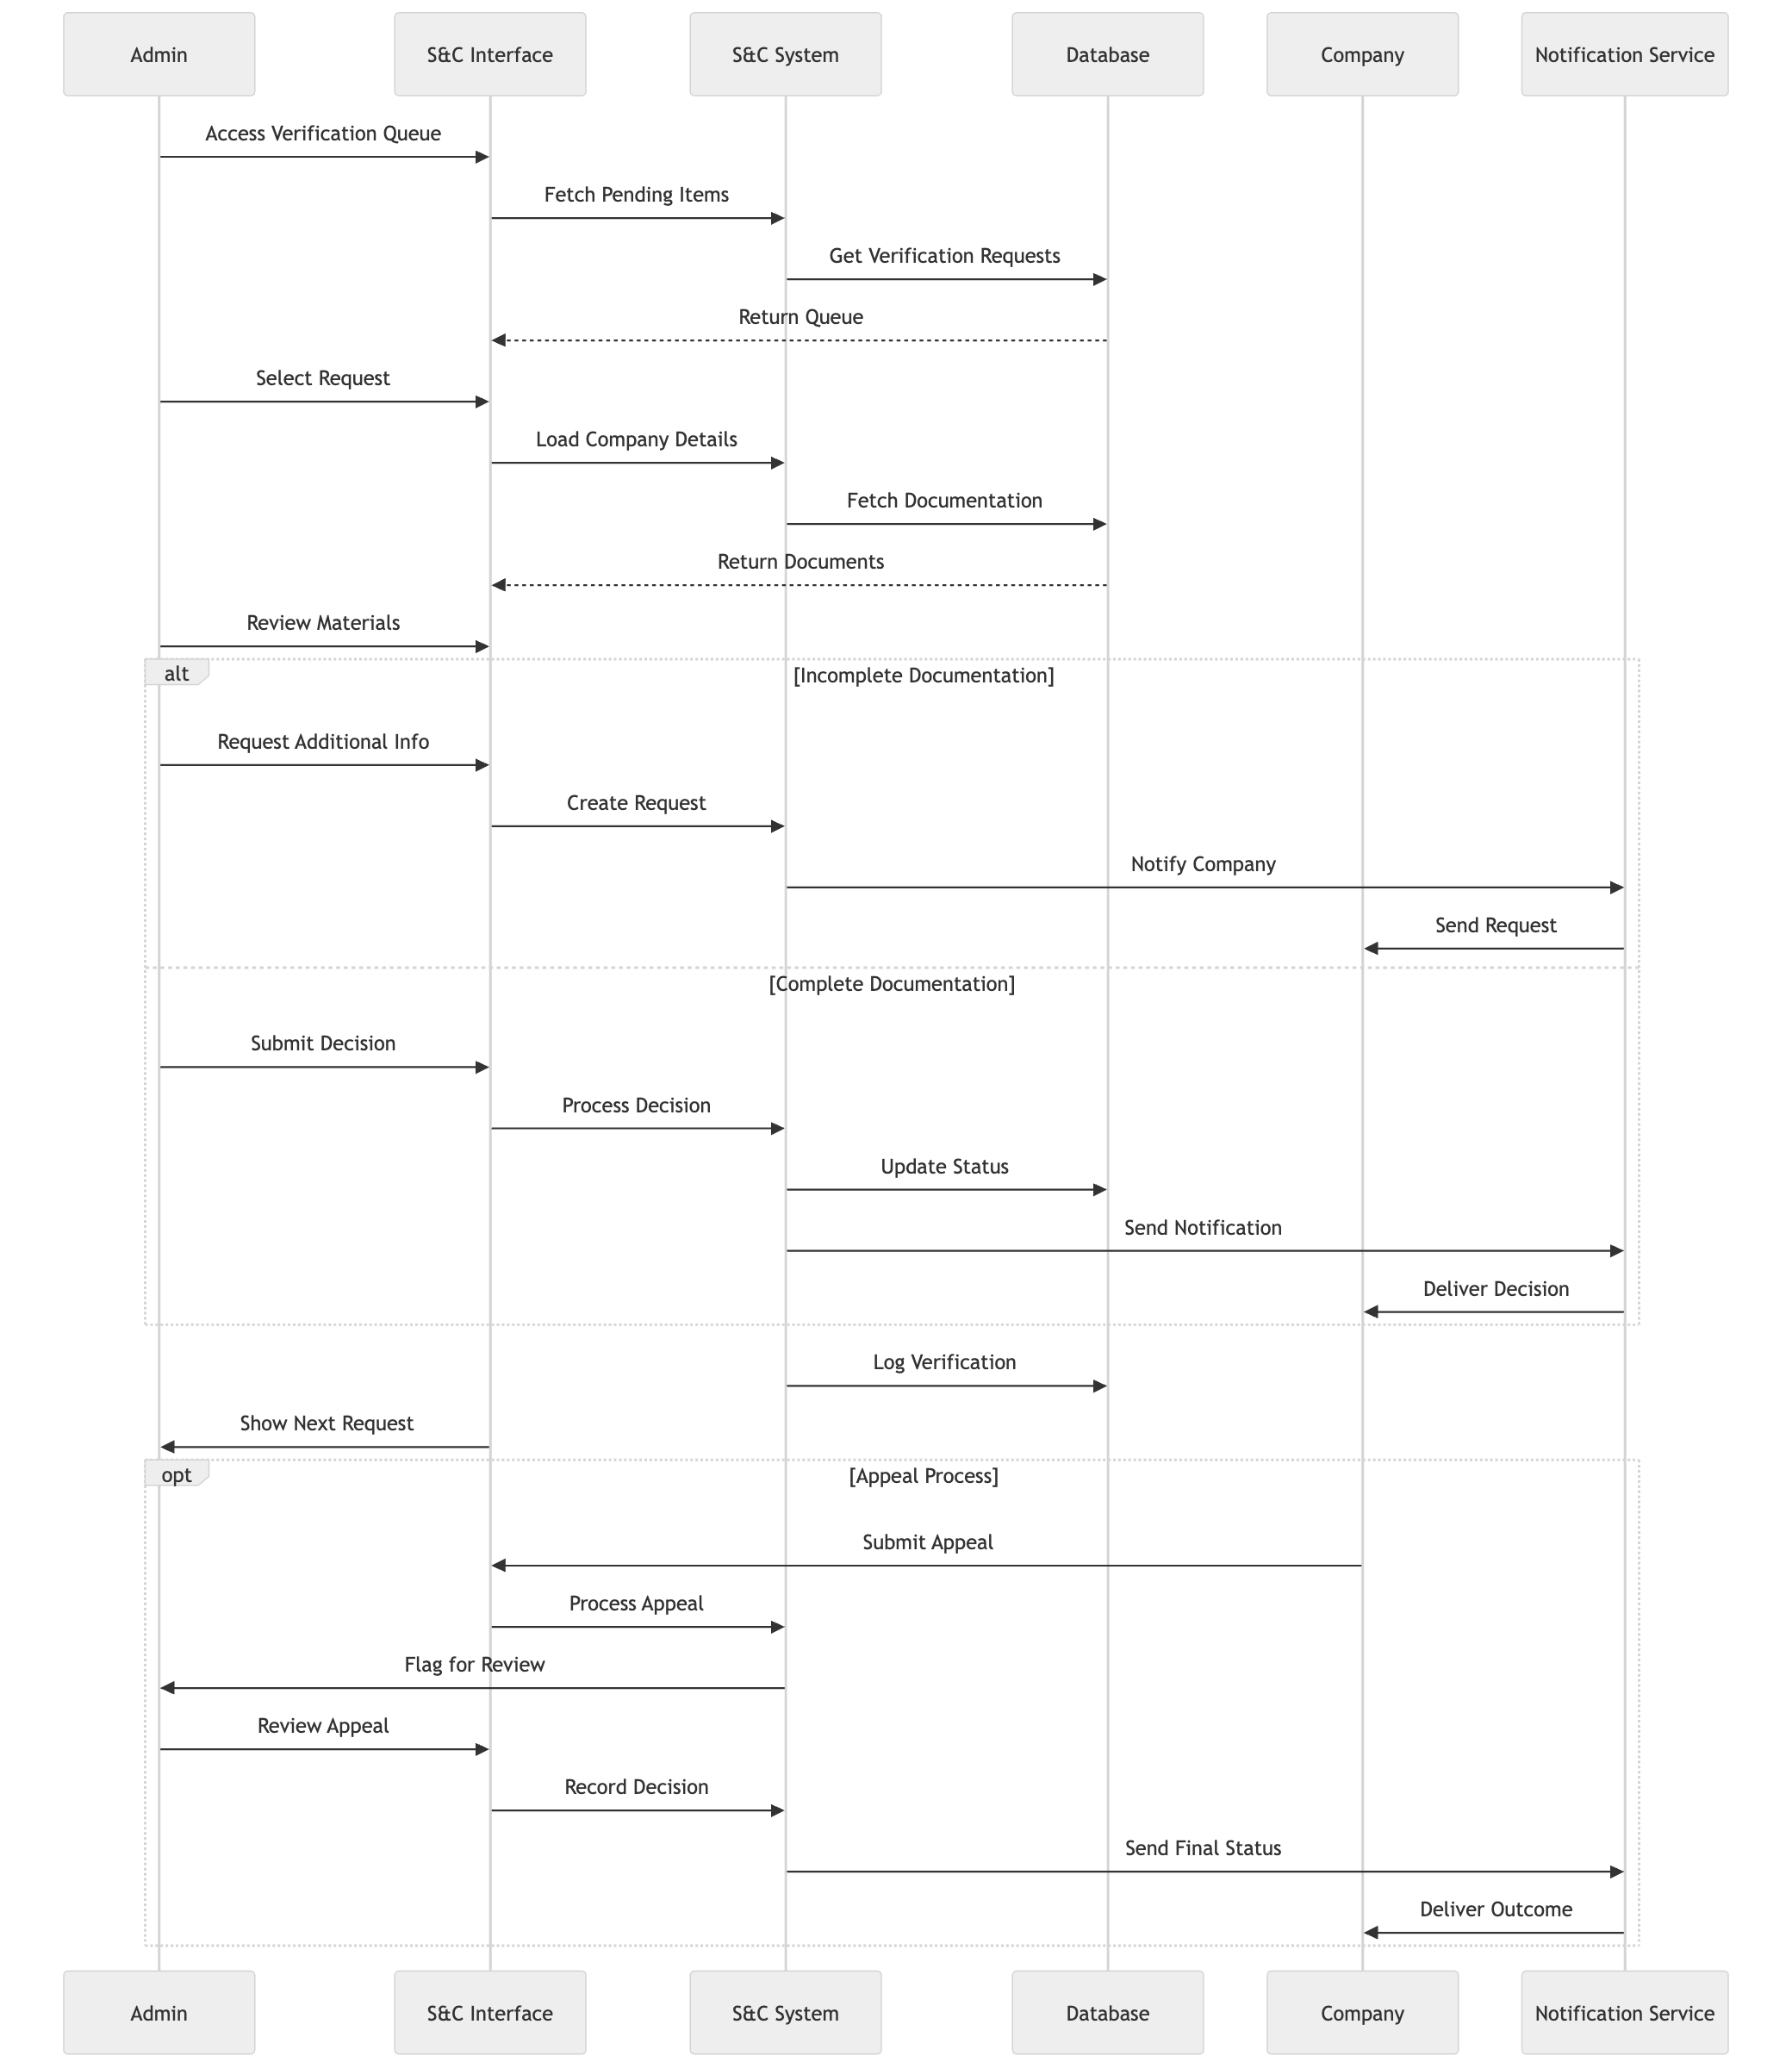
\includegraphics[width=1\linewidth]{JhaBhatiaSharma/Images/Sequence Diagrams/AdminPriviliges.png}
        \caption{Sequence Diagram for Admin Privileges}
        \label{fig:adminPrivileges}%
    \end{center}
\end{figure}
\newpage

\subsection{Performance Requirements}
\label{subsec:performance_requirements}

\subsubsection*{Response Time}
\begin{itemize}
    \item \textbf{Page Load:} Less than \textbf{5 seconds} for typical pages during testing.
    \item \textbf{Search Results:} Less than \textbf{2 seconds} for small-scale datasets.
    \item \textbf{File Upload:} Less than \textbf{10 seconds} for files up to \textbf{10MB}.
    \item \textbf{Real-time Updates:} Less than \textbf{1 second} for key interactive features.
\end{itemize}

\subsubsection*{System Capacity}
\begin{itemize}
    \item \textbf{Concurrent Users:} Support for up to \textbf{50 simultaneous users}.
    \item \textbf{Database Transactions:} Designed to handle \textbf{10 transactions per second} under typical usage.
    \item \textbf{File Storage:} Capacity for up to \textbf{10GB}, suitable for project scope and testing.
    \item \textbf{Backup Frequency:} \textbf{Weekly or manual backups} for data protection during development.
\end{itemize}

\subsubsection*{Availability}
\begin{itemize}
    \item \textbf{Uptime:} \textbf{Target of 95\%}, considering potential downtime for development and testing.
    \item \textbf{Scheduled Maintenance:} As needed during the project lifecycle.
    \item \textbf{Backup Recovery:} Recovery within \textbf{12 hours for small-scale data}.
    \item \textbf{Error Rate:} Less than \textbf{1\% for prototype-level functionality}.
\end{itemize}


\newpage
\section{Design constraints}
\label{sec:design_constraints}%


\subsection{Design Constraints}
\label{subsec:design_constraints}

\subsubsection*{Standards Compliance}
\begin{itemize}
    \item \textbf{GDPR Compliance:} 
    The platform must comply with the \textbf{General Data Protection Regulation} to ensure the protection of user data and privacy. This includes explicit consent mechanisms, data anonymization, and secure data processing protocols.
    \item \textbf{WCAG 2.1 Accessibility:} 
    Adheres to the \textbf{Web Content Accessibility Guidelines 2.1} to ensure inclusivity. This involves providing support for screen readers, keyboard navigation, and ensuring sufficient color contrast.
    \item \textbf{ISO/IEC 27001 Security:} 
    Implements security management practices aligned with \textbf{ISO/IEC 27001} to safeguard information assets and prevent data breaches. This includes encryption, secure authentication, and incident response planning.
    \item \textbf{Browser Standards:} 
    Ensures \textbf{cross-browser compatibility} by adhering to \textbf{HTML5, CSS3, and modern JavaScript standards}. This allows the platform to work seamlessly on popular browsers like Chrome, Firefox, and Edge.
\end{itemize}

\subsubsection*{Development Constraints}
\begin{itemize}
    \item \textbf{Web-based Architecture:} 
    The system will be fully web-based, designed to run on a server and accessible via web browsers without the need for additional software installations.
    \item \textbf{Responsive Design:} 
    The platform must be responsive, ensuring an optimal user experience on devices of varying screen sizes, including desktops, tablets, and mobile phones.
    \item \textbf{Modular Components:} 
    The architecture will be modular, facilitating easier debugging, testing, and future enhancements by breaking functionality into independent, reusable components.
    \item \textbf{API-First Approach:} 
    Development will follow an API-first methodology, prioritizing a well-documented API layer that enables easy integration with external systems and scalability for future mobile app development.
\end{itemize}

\newpage
\subsection{Software System Attributes}
\label{subsec:software_system_attributes}

\subsubsection*{Reliability}
\begin{itemize}
    \item \textbf{Error handling} to ensure data integrity.
    \item \textbf{Input validation} for all user entries.
    \item \textbf{Transaction integrity} for financial processes.
    \item \textbf{System recovery} after failures.
\end{itemize}

\subsubsection*{Availability}
\begin{itemize}
    \item \textbf{Redundant Systems:} Ensure continuous, round-the-clock functioning of the platform.
    \item \textbf{Failover Mechanism:} Enables the system to handle server disruptions by automatically switching to backup systems.
\end{itemize}

\subsubsection*{Security}
\begin{itemize}
    \item \textbf{Robust} authentication systems.
    \item \textbf{Authorization for sensitive operations} based on roles.
    \item \textbf{Data encryption} from beginning to end.
\end{itemize}

\subsubsection*{Maintainability}
\begin{itemize}
    \item \textbf{Modular design} for easier updates.
    \item \textbf{Comprehensive documentation} for developers and users.
    \item \textbf{Version control} for all software components.
    \item \textbf{Automated testing} frameworks.
\end{itemize}

\subsubsection*{Portability}
\begin{itemize}
    \item \textbf{Cross-browser} compatibility.
    \item \textbf{Mobile responsiveness.}
    \item \textbf{Platform independence} to run on various operating systems.
    \item \textbf{Easy deployment} for scaling and updates.
\end{itemize}




    \chapter{Requirements Traceability} \label{ch:requirements_tracability}%
    \section{System Requirements}
\label{sec:system_requirements}

This section outlines the functional requirements of the InternHub – Students \& Companies (S\&C) platform, categorized by the major system components.

\subsection{Login Manager}
\label{subsec:login_manager}
\begin{enumerate}[label=R\arabic*:, itemsep=0.2em]
    \item The system allows registered students to log in.
    \item The system allows registered companies to log in.
    \item The system ensures secure access to accounts through credential verification.
    \item The system validates user input during login.
    \item The system provides error messages for invalid credentials.
\end{enumerate}

\subsection{Registration Manager}
\label{subsec:registration_manager}
\begin{enumerate}[label=R\arabic*:, itemsep=0.2em, start=6]
    \item The system allows unregistered users (students and companies) to sign up.
    \item The system verifies user details before creating accounts.
    \item The system communicates with the mailing system to send verification emails during registration.
    \item The system ensures unique email addresses during registration.
    \item The system allows recruiters to register company profiles with required information fields.
\end{enumerate}

\subsection{Internship Manager}
\label{subsec:internship_manager}
\begin{enumerate}[label=R\arabic*:, itemsep=0.2em, start=11]
    \item The system allows companies to create new internship postings.
    \item The system allows companies to update existing internship details.
    \item The system enables recruiters to delete internships.
    \item The system fetches all internship postings associated with a specific recruiter.
    \item The system provides students with the ability to search and filter internships based on preferences.
    \item The system supports adding multiple job roles under a single internship posting.
    \item The system tracks the total number of internships posted by a company.
\end{enumerate}

\subsection{Application Manager}
\label{subsec:application_manager}
\begin{enumerate}[label=R\arabic*:, itemsep=0.2em, start=18]
    \item The system allows students to submit applications for internships.
    \item The system enables recruiters to review student applications.
    \item The system tracks the status of submitted applications.
    \item The system supports updating the status of an application (e.g., accepted, rejected).
    \item The system provides recruiters with filters to search through applications.
    \item The system notifies students of changes in their application status.
\end{enumerate}

\subsection{Interview Manager}
\label{subsec:interview_manager}
\begin{enumerate}[label=R\arabic*:, itemsep=0.2em, start=24]
    \item The system allows recruiters to schedule interviews for shortlisted candidates.
    \item The system notifies students of upcoming interviews.
    \item The system tracks interview details and schedules.
    \item The system sends reminders to students and recruiters for scheduled interviews.
    \item The system allows students to view interview details, including time and interviewer.
    \item The system supports rescheduling of interviews by recruiters.
\end{enumerate}

\subsection{Complaint Manager}
\label{subsec:complaint_manager}
\begin{enumerate}[label=R\arabic*:, itemsep=0.2em, start=30]
    \item The system allows users (students and companies) to file complaints regarding issues.
    \item The system ensures proper logging of all complaints for administrative review.
    \item The system enables administrators to resolve complaints and update their status.
    \item The system notifies users about updates to their complaints.
    \item The system maintains a history of resolved complaints for audit purposes.
\end{enumerate}

\subsection{Profile Manager}
\label{subsec:profile_manager}
\begin{enumerate}[label=R\arabic*:, itemsep=0.2em, start=35]
    \item The system allows students to manage their profiles, including uploading resumes and updating details.
    \item The system allows companies to manage their profiles and update organization details.
    \item The system supports the ability to view profiles of other users (students or companies).
    \item The system provides recommendations for internships based on student profiles.
    \item The system highlights incomplete profiles for users and prompts them to complete missing details.
\end{enumerate}

\subsection{Search and Filter}
\label{subsec:search_and_filter}
\begin{enumerate}[label=R\arabic*:, itemsep=0.2em, start=40]
    \item The system provides students and companies with advanced search and filter options for internships, candidates, or postings.
    \item The system ensures search results are relevant and aligned with user preferences.
    \item The system supports search by location, duration, stipend, and skills.
    \item The system allows recruiters to filter student applications by skills and experience.
    \item The system enables sorting of search results by relevance or other criteria.
\end{enumerate}

\subsection{Dashboard Manager}
\label{subsec:dashboard_manager}
\begin{enumerate}[label=R\arabic*:, itemsep=0.2em, start=45]
    \item The system provides students with an overview of their active applications, upcoming interviews, and recent internship matches.
    \item The system provides companies with an overview of active postings, total applicants, and scheduled interviews.
    \item The system allows administrators to monitor platform activities, including user engagement and complaint handling.
    \item The system displays key metrics for students, such as total applications and new messages.
    \item The system allows companies to see statistics on applicants and hires.
\end{enumerate}

\subsection{Notification Manager}
\label{subsec:notification_manager}
\begin{enumerate}[label=R\arabic*:, itemsep=0.2em, start=50]
    \item The system sends notifications to students when their application status is updated.
    \item The system notifies students and companies of scheduled interviews.
    \item The system sends reminders for upcoming deadlines, including applications and interviews.
    \item The system notifies users about updates to their complaints.
    \item The system alerts students about new internship matches based on their profiles.
\end{enumerate}

\subsection{Model}
\label{subsec:model}
\begin{enumerate}[label=R\arabic*:, itemsep=0.2em, start=55]
    \item The system securely stores user data, including profiles, applications, and complaints.
    \item The system ensures the integrity and security of all data through encryption and access controls.
    \item The system logs all user actions for security and audit purposes.
    \item The system supports scalable storage for managing increasing user data.
    \item The system ensures efficient data retrieval for dashboard and search functionalities.
\end{enumerate}


 \chapter{Implementation, Integration and Test Plan}
\label{ch:implementation_integration_test_plan}
\section{Overview and Implementation Plan}
\label{sec:overview_implementation}

This chapter describes the InternHub – Students \& Companies (S\&C) platform's integration strategy, test plan, and implementation procedure. A systematic and effective development process will be ensured by using the \textbf{Bottom-Up approach}.

The implementation will start with basic, independent modules that do not need additional modules to work. Drivers for testing each module separately will be created. Modules will gradually be added to the system, taking the place of their associated drivers as they are implemented and tested. For further testing, each integrated module will need its own driver.

Before a system is fully integrated, smaller functional subsystems can be created using the Bottom-Up approach. With this incremental approach:
\begin{itemize}
    \item Testing is performed on smaller parts of the system initially and continues for each module as it becomes ready, making debugging and error tracking easier.
    \item Parallel development is facilitated, allowing separate teams to work on various elements simultaneously.
\end{itemize}

\section{Features Identification}
\label{sec:features_identification}

The features of the platform are prioritized based on their dependencies and importance, as outlined below:

\subsection{[F1] Login and Registration Features}
\begin{itemize}
    \item These are the core features required for students, companies, and administrators to access the platform.
    \item Include user registration, login, and secure authentication.
    \item As foundational features, they will be implemented first to support the functioning of subsequent features.
\end{itemize}

\subsection{[F2] Profile Management Features}
\begin{itemize}
    \item This set of features includes creating and managing profiles for students, companies, and administrators.
    \item Students can update personal details, upload CVs, and showcase skills.
    \item Companies can maintain organization profiles.
    \item These features serve as the foundation for the search and application functionalities.
\end{itemize}

\subsection{[F3] Internship Management Features}
\begin{itemize}
    \item Includes the ability for companies to create, update, and delete internship postings.
    \item Involves managing applications received for these internships.
    \item Requires proper implementation of profile management ([F2]).
    \item Will be developed subsequently after [F1] and [F2].
\end{itemize}

\subsection{[F4] Search and Filter Features}
\begin{itemize}
    \item Includes advanced search and filter functionalities:
    \begin{itemize}
        \item Students can find relevant internships.
        \item Companies can search through applicants.
    \end{itemize}
    \item These features depend on the successful implementation of profile and internship management ([F2] and [F3]).
\end{itemize}

\subsection{[F5] Application and Interview Features}
\begin{itemize}
    \item Includes submitting applications, reviewing them, scheduling interviews, and notifying users about interview updates.
    \item These features depend on internship management ([F3]) and profile management ([F2]).
\end{itemize}

\subsection{[F6] Complaint Handling Features}
\begin{itemize}
    \item Allows students and companies to lodge complaints and administrators to review and resolve them.
    \item Ensures user satisfaction and platform reliability.
    \item Relies on the proper implementation of profile management ([F2]) and dashboard functionalities ([F8]).
\end{itemize}

\subsection{[F7] Notification Features}
\begin{itemize}
    \item Ensures that students, companies, and administrators are notified about critical events:
    \begin{itemize}
        \item Interview schedules.
        \item Application updates.
        \item Complaint resolutions.
    \end{itemize}
    \item These features will be developed last as they depend on the correct functioning of all other features.
\end{itemize}

\subsection{[F8] Dashboard Features}
\begin{itemize}
    \item The dashboard provides an overview of active internships, applications, interviews, and platform activities for students, companies, and administrators.
    \item Consolidates data from various modules.
    \item Critical for system usability.
\end{itemize}

\subsection{Development Dependencies}
\label{subsec:development_dependencies}

The dependencies between the features ensure a structured and incremental implementation:
\begin{enumerate}
    \item [F1] Login and Registration Features serve as the foundation for all other functionalities.
    \item [F2] Profile Management Features are prerequisites for Internship Management ([F3]) and Search and Filter ([F4]).
    \item [F3] Internship Management Features depend on Profile Management ([F2]) and support Application and Interview Features ([F5]).
    \item [F4] Search and Filter Features depend on both Profile Management ([F2]) and Internship Management ([F3]).
    \item [F5] Application and Interview Features depend on Profile Management ([F2]), Internship Management ([F3]), and Search and Filter ([F4]).
    \item [F6] Complaint Handling Features rely on Profile Management ([F2]) and Dashboard Features ([F8]).
    \item [F7] Notification Features depend on the correct functioning of all other features.
    \item [F8] Dashboard Features consolidate data from all modules and rely on their successful implementation.
\end{enumerate}

This dependency-based plan ensures that features are developed systematically, reducing errors and facilitating incremental testing.

\section{Implementation Strategy}
\label{subsec:implementation_strategy}

\subsection{Overview and Integration Plan}
\label{subsubsec:integration_plan}

A systematic \textbf{bottom-up method} is used to integrate the system's components. The emphasis will be on developing solid foundational modules that can be gradually combined, starting with the essential elements. Before each module is integrated into the larger system, it will be tested using the relevant drivers. This approach enables:
\begin{itemize}
    \item Parallel programming.
    \item Effective debugging.
    \item Incremental functional validation.
\end{itemize}

The following crucial areas will be included in the integration process:

\paragraph{Core Model Integration}

The core model integration serves as the system's cornerstone, incorporating the data models necessary for the platform's operation. These include:
\begin{itemize}
    \item \textbf{User Model:} Manages user-related information.
    \item \textbf{Resume Model:} Handles CVs and profile details.
    \item \textbf{Internship Model:} Stores internship data.
    \item \textbf{Application Model:} Tracks internship applications.
    \item \textbf{Interview Model:} Manages interview scheduling and feedback.
    \item \textbf{Complaint Model:} Logs and tracks complaints.
\end{itemize}
\begin{figure}[H]
    \begin{center}
        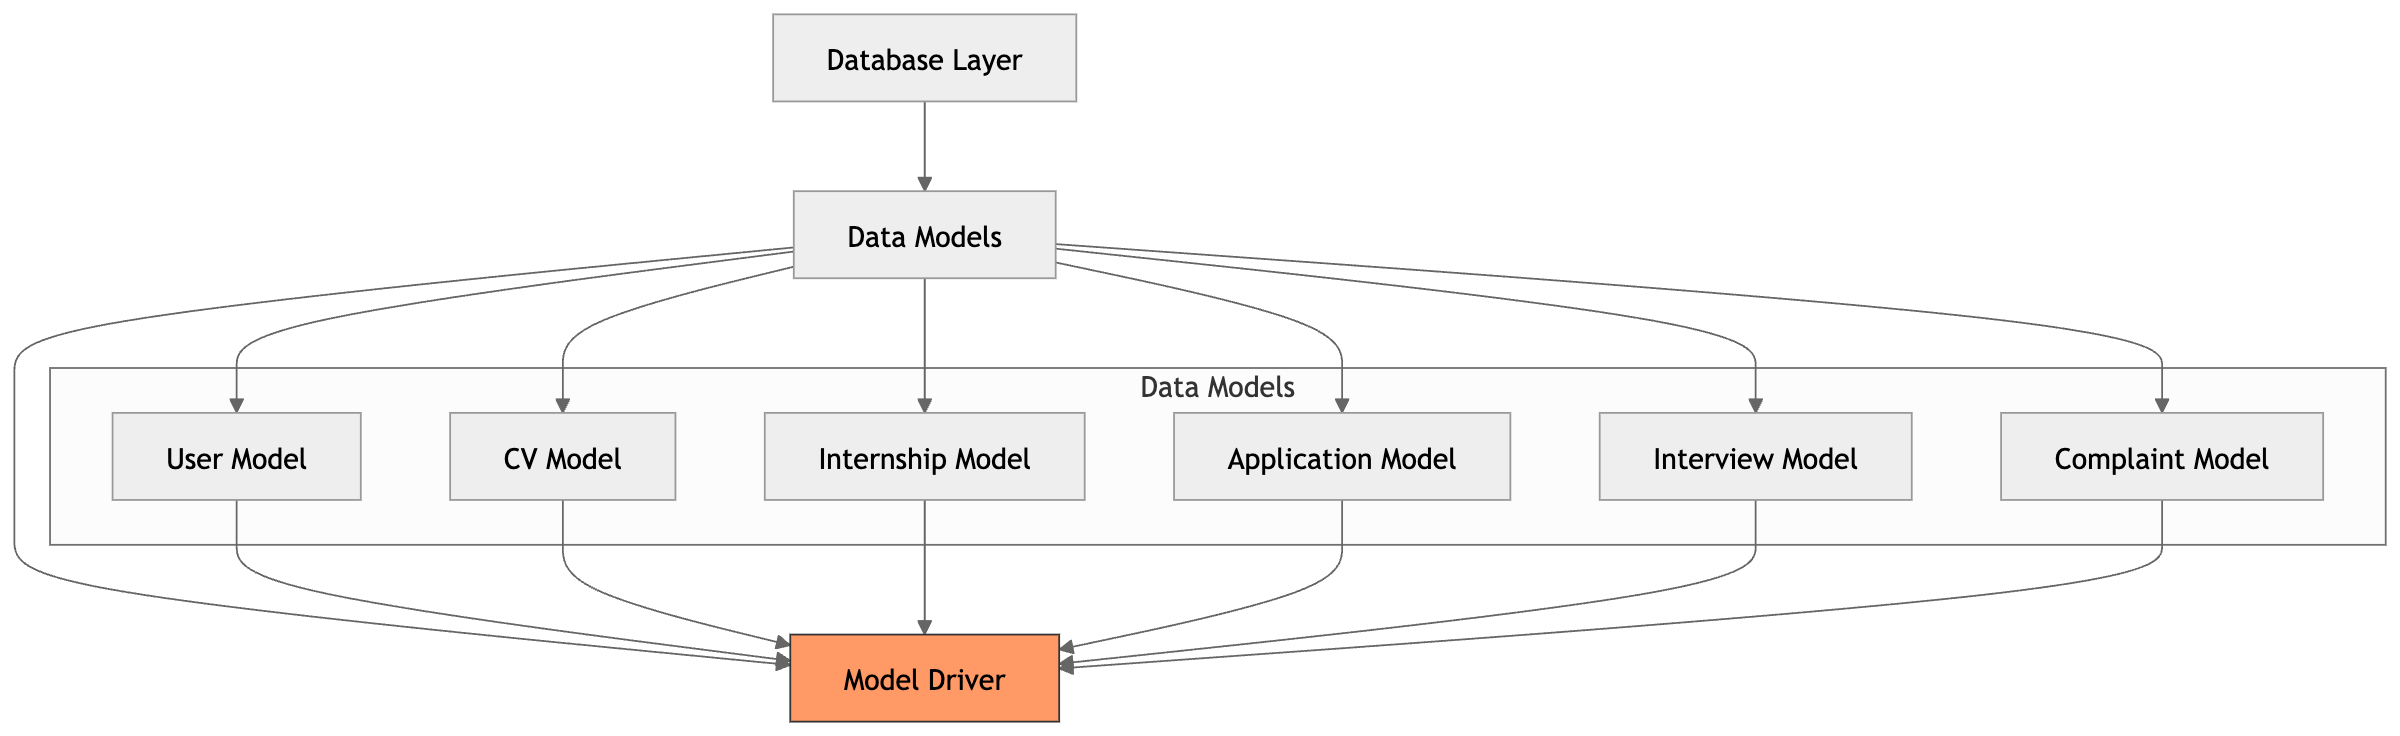
\includegraphics[width=0.79\linewidth]{JhaBhatiaSharma/imagesDD/CoreModelIntegration.png}
        \caption{Core Model Integration}
        \label{fig:coreModelIntegration}
    \end{center}
\end{figure}
Each model will communicate with the database layer to perform CRUD operations and ensure data consistency and integrity. A \textbf{Model Driver} will be implemented to test these models individually and verify their efficient interaction with the database layer. Once validated, these models will be integrated into their corresponding manager components.

\paragraph{Authentication Integration}

Authentication integration focuses on user registration and login procedures. The \textbf{Authentication Manager} will handle interactions between the data models and the user interfaces for registration and login. Key functionalities include:
\begin{itemize}
    \item Secure communication with the Registration System.
    \item Data validation.
    \item Access token generation.
    \item Credential validation workflows.
\end{itemize}
\begin{figure}[H]
    \begin{center} 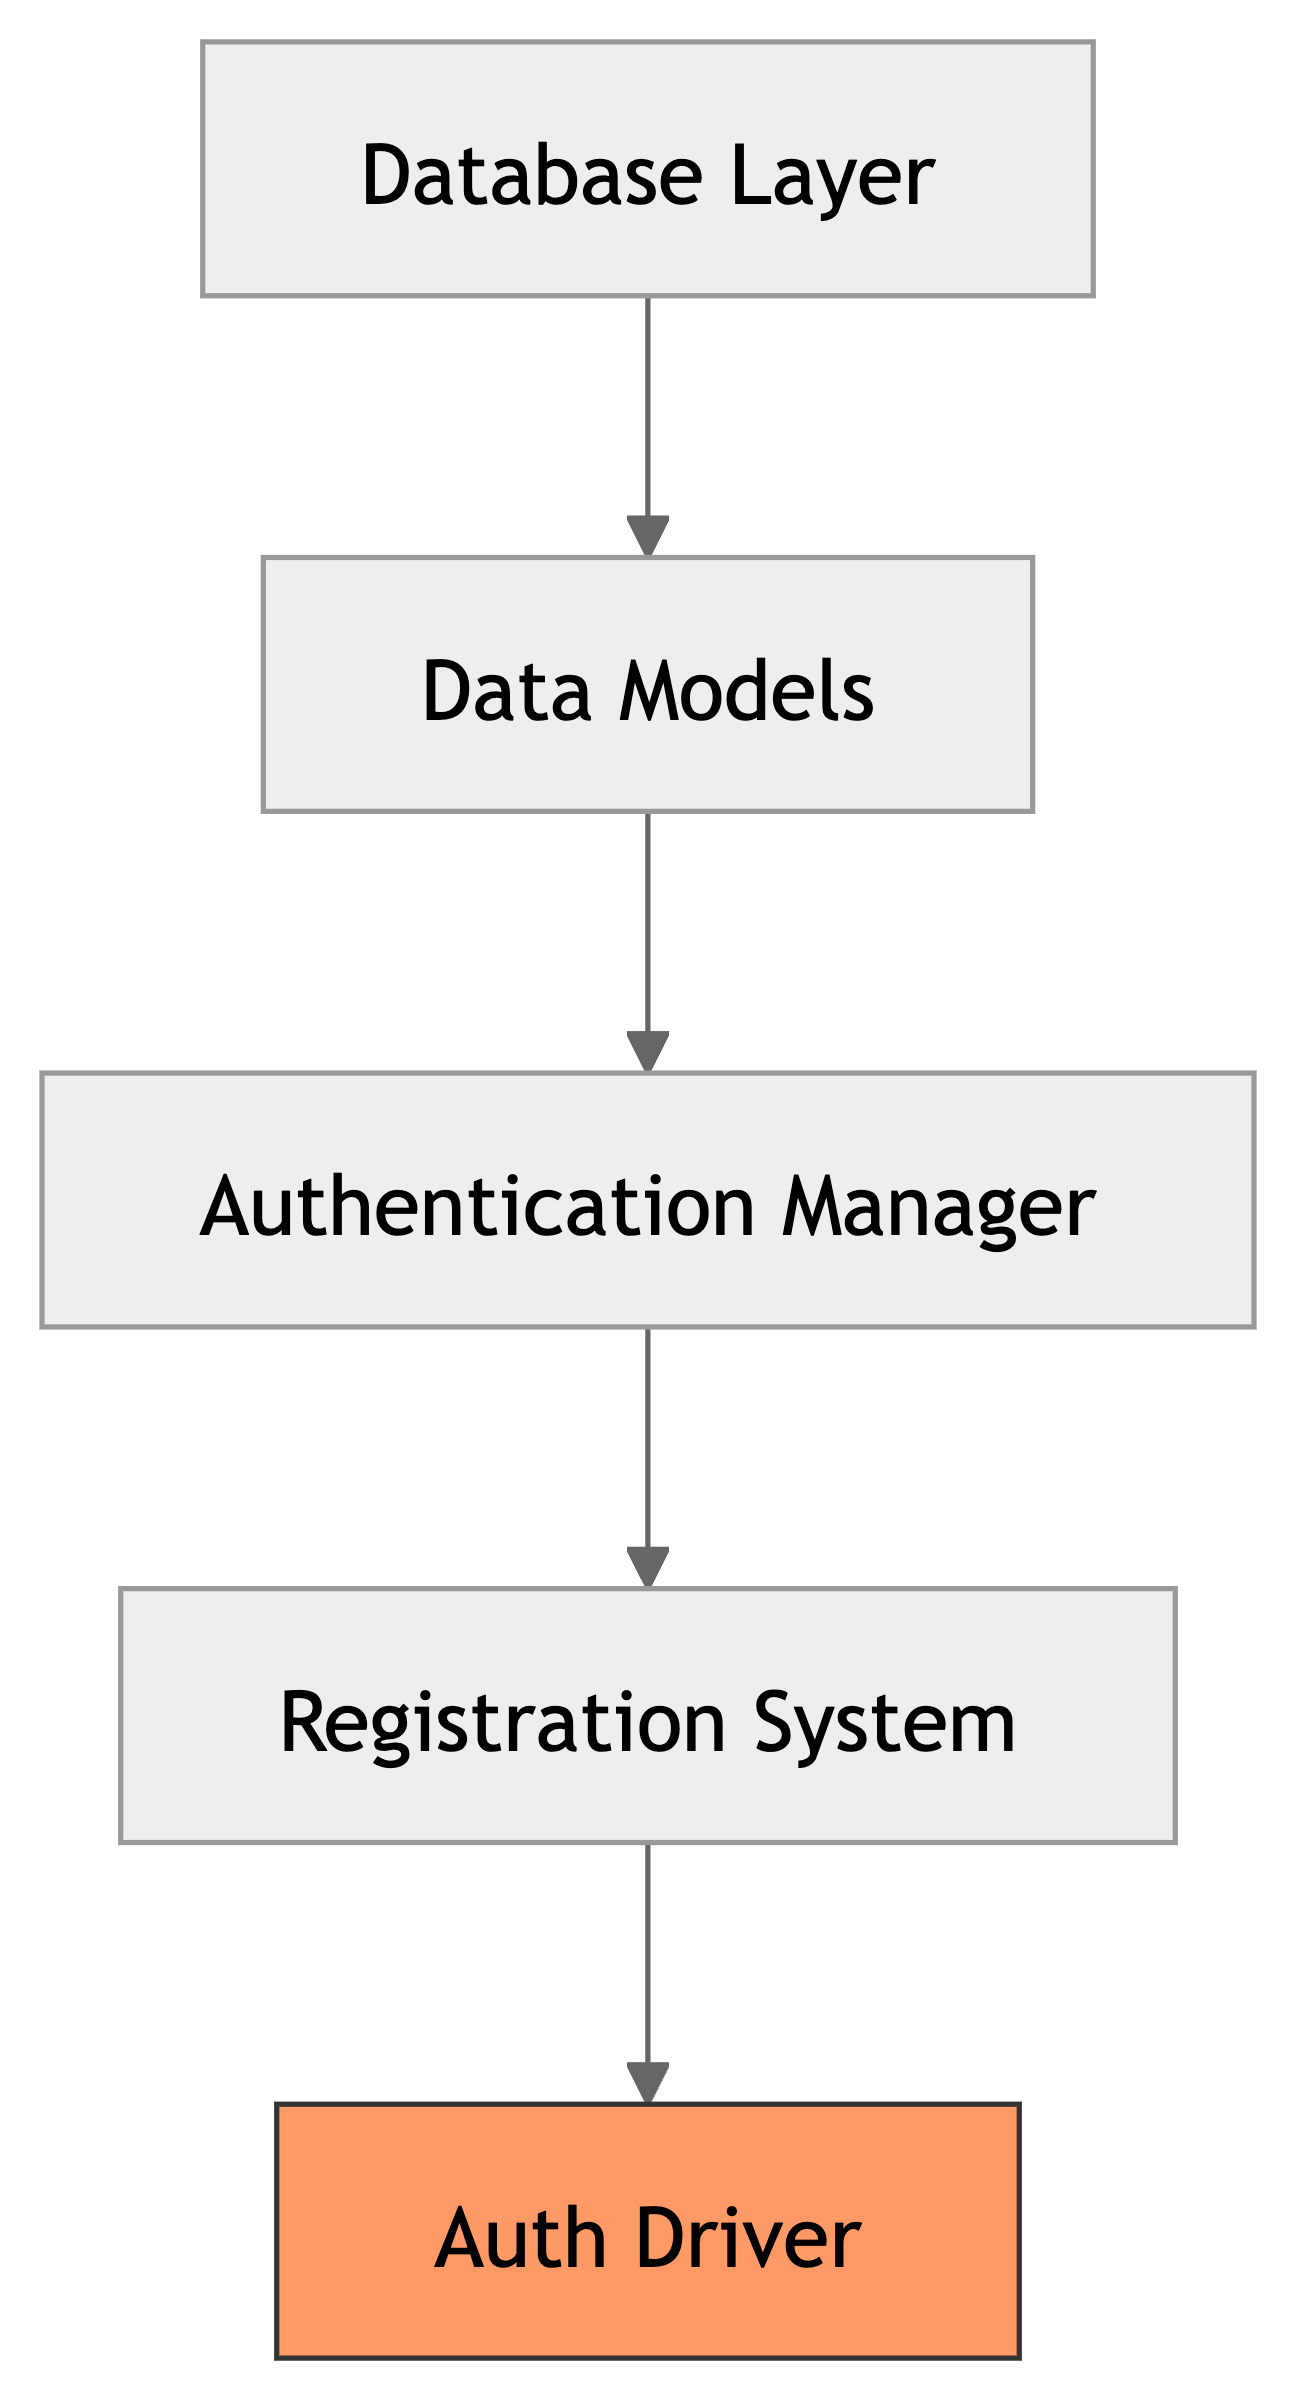
\includegraphics[width=0.18\linewidth]{JhaBhatiaSharma/imagesDD/AuthenticationIntegration.png}
    \caption{Authentication Integration}
        \label{fig:authenticationIntegration}
    \end{center}
\end{figure}

A driver will test the authentication workflows, ensuring stability before integrating the Authentication Manager with the larger system to facilitate secure user authentication and seamless login.

\paragraph{Profile Management Integration}
The \textbf{Profile Manager} handles the creation and management of profiles for administrators, companies, and students. This module will interact directly with the Authentication Manager to ensure only authorized users can manage profiles. Key features include:
\begin{itemize}
    \item Profile creation.
    \item Profile editing.
    \item Profile retrieval.
\end{itemize}
\begin{figure}[H]
    \begin{center}
        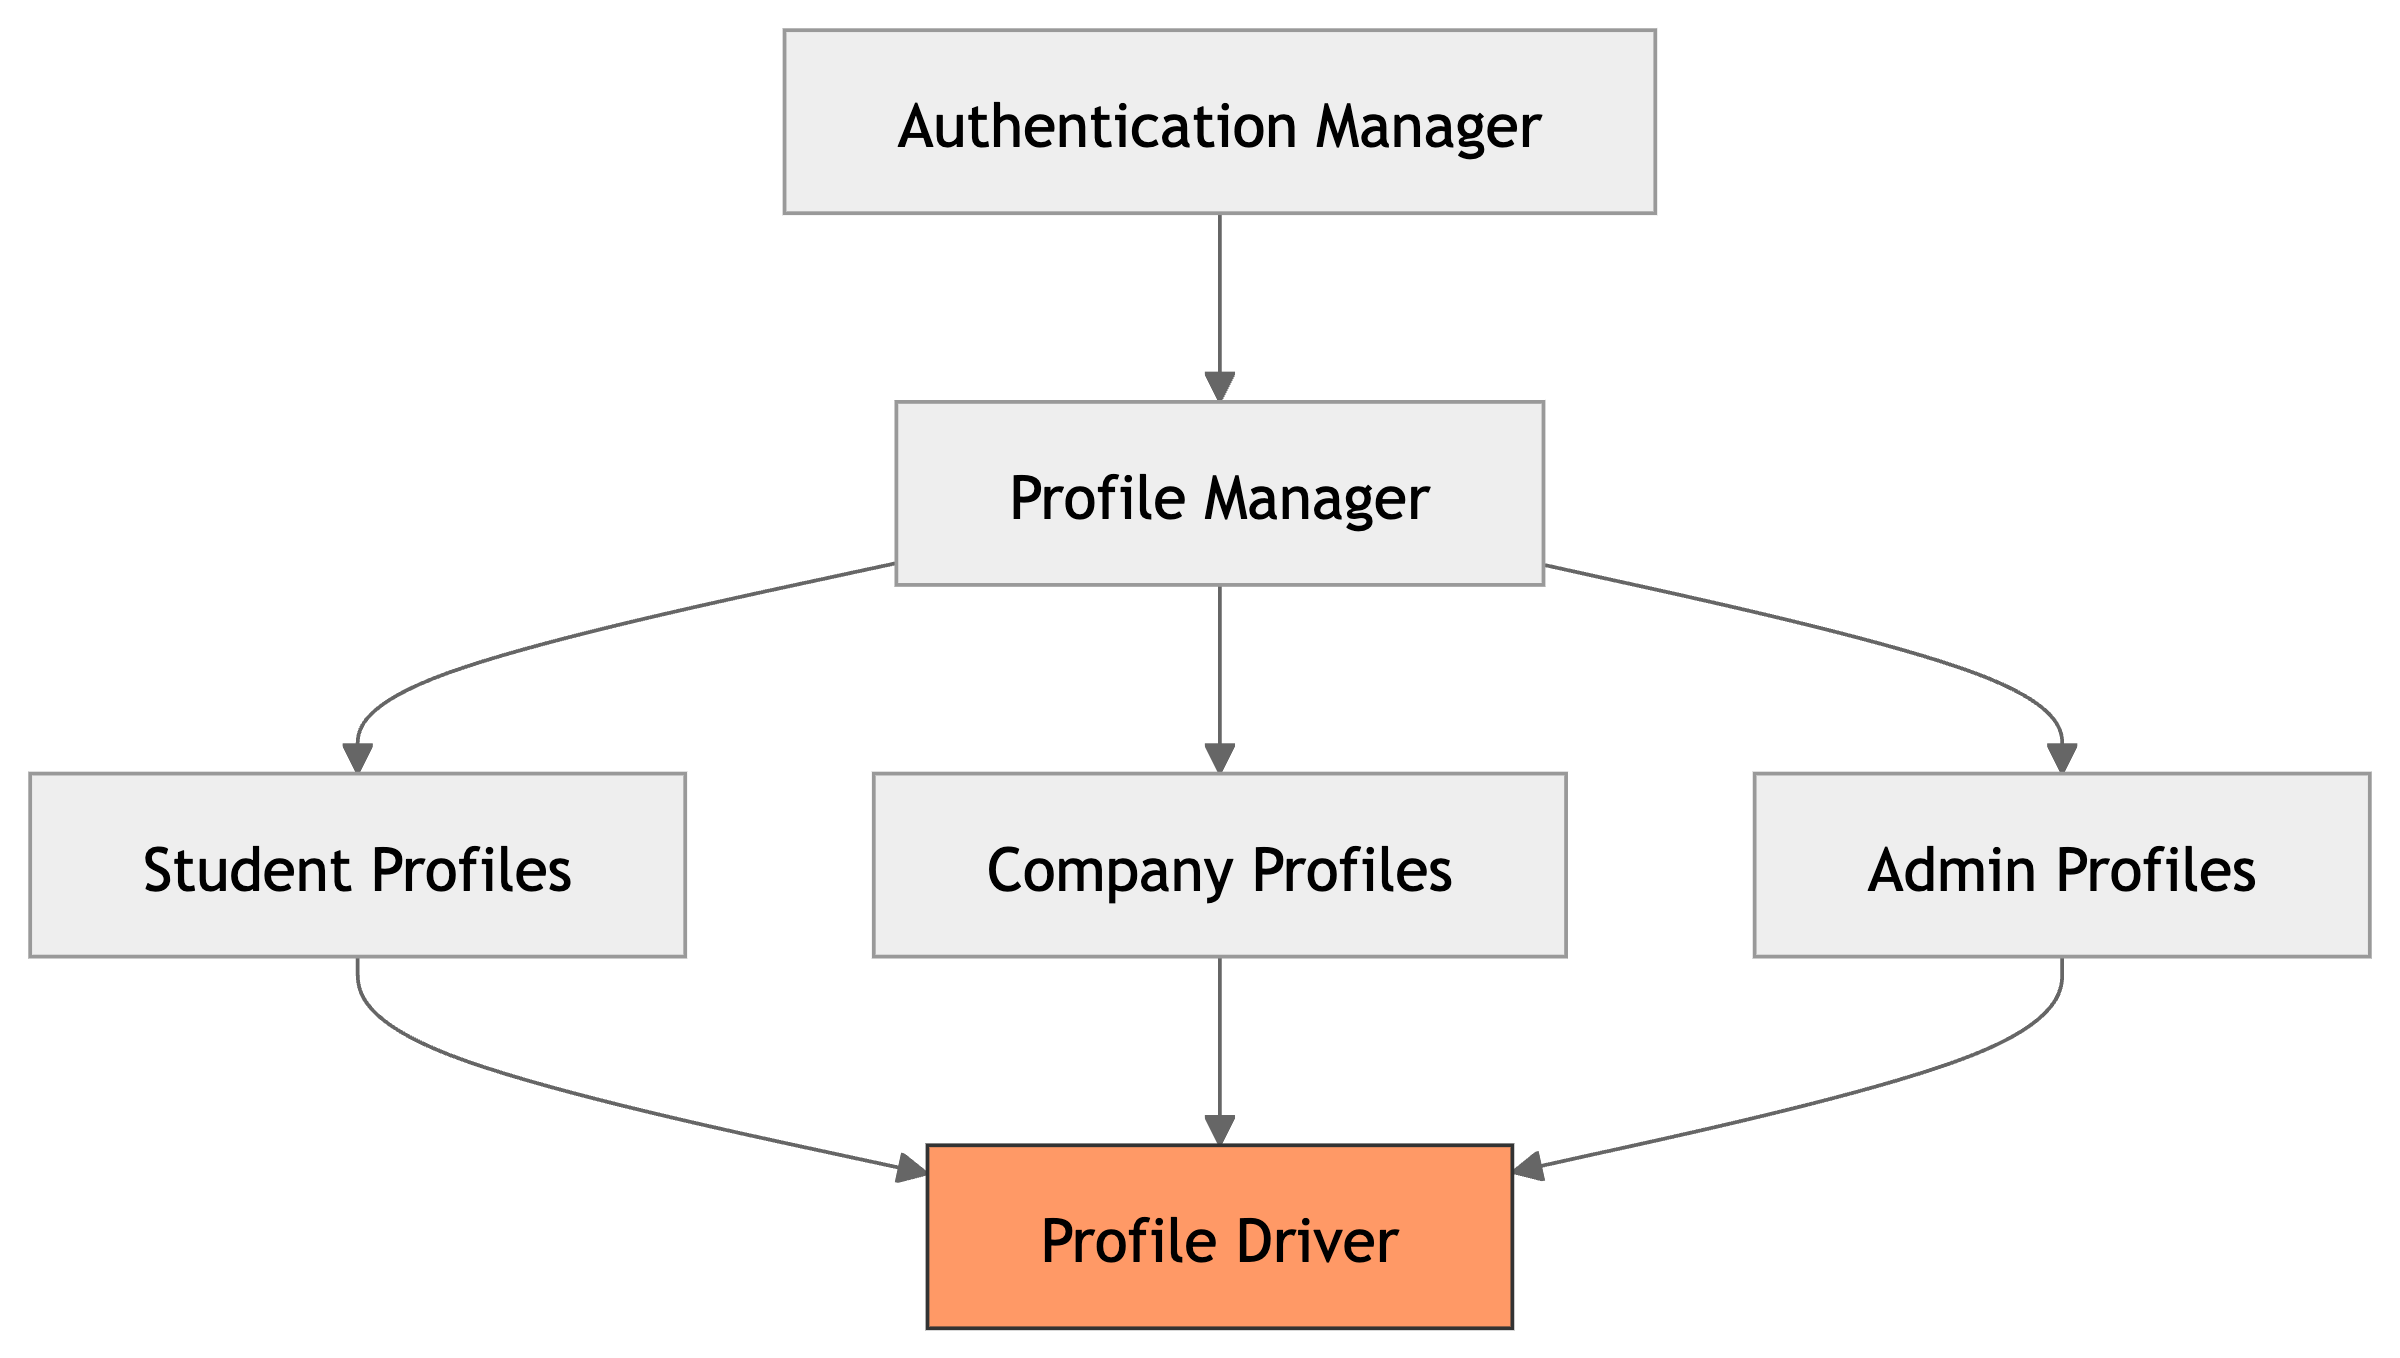
\includegraphics[width=0.79\linewidth]{JhaBhatiaSharma/imagesDD/ProfileIntegration.png}
        \caption{Profile Management Integration}
        \label{fig:profileManagement}
    \end{center}
\end{figure}
The \textbf{Profile Driver} will test these features to validate functionality. This integration is critical for enabling personalized user experiences and creating user identification across the platform.

\paragraph{Internship Management Integration}
The \textbf{Internship Manager} is central to coordinating the posting and management of internship opportunities. It integrates with:
\begin{itemize}
    \item The Profile Manager to verify recruiter responsibilities and permissions.
    \item The Application System to manage student applications and facilitate filtering and internship searches.
\end{itemize}
\begin{figure}[H]
    \begin{center}
        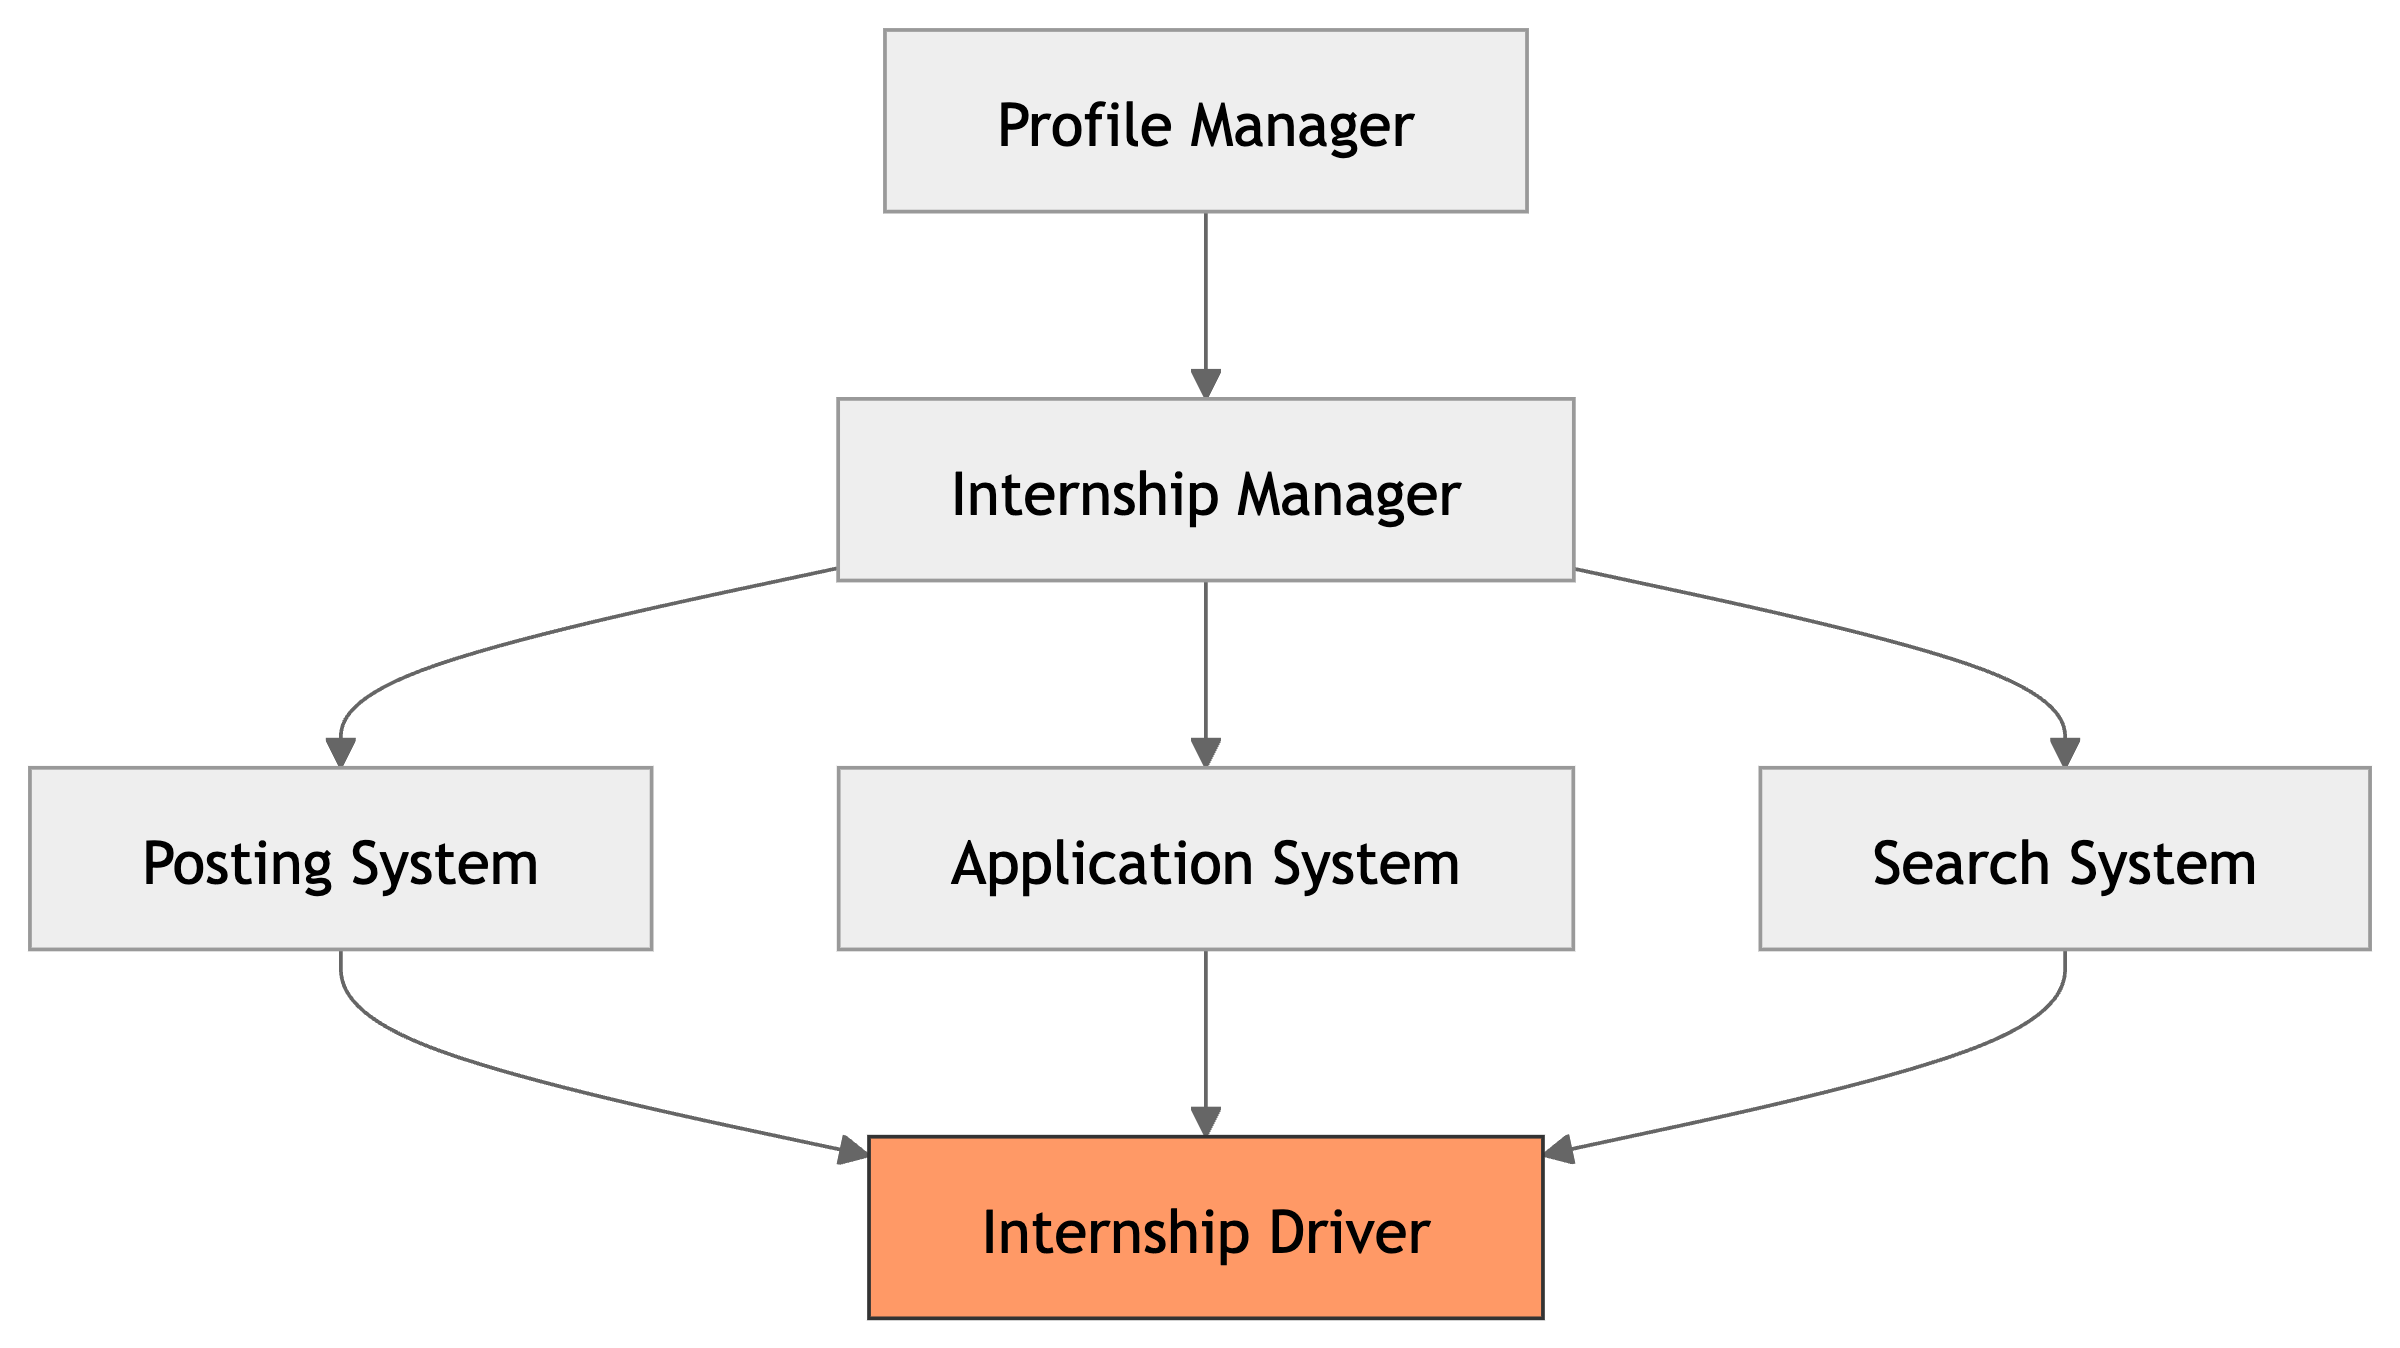
\includegraphics[width=0.79\linewidth]{JhaBhatiaSharma/imagesDD/InternshipManagementIntegration.png}
        \caption{Internship Management Integration}
        \label{fig:internshipManagement}
    \end{center}
\end{figure}
A driver will test functionalities such as posting, deleting, and searching for internships to ensure safe and effective internship management.

\paragraph{Interview and Communication Integration}
The \textbf{Interview Manager} and \textbf{Communication Manager} are responsible for interview scheduling and stakeholder communication. The integration includes:
\begin{itemize}
    \item The Scheduling System to handle interview setups.
    \item The Feedback System to collect post-interview feedback.
\end{itemize}
\begin{figure}[H]
    \begin{center}
        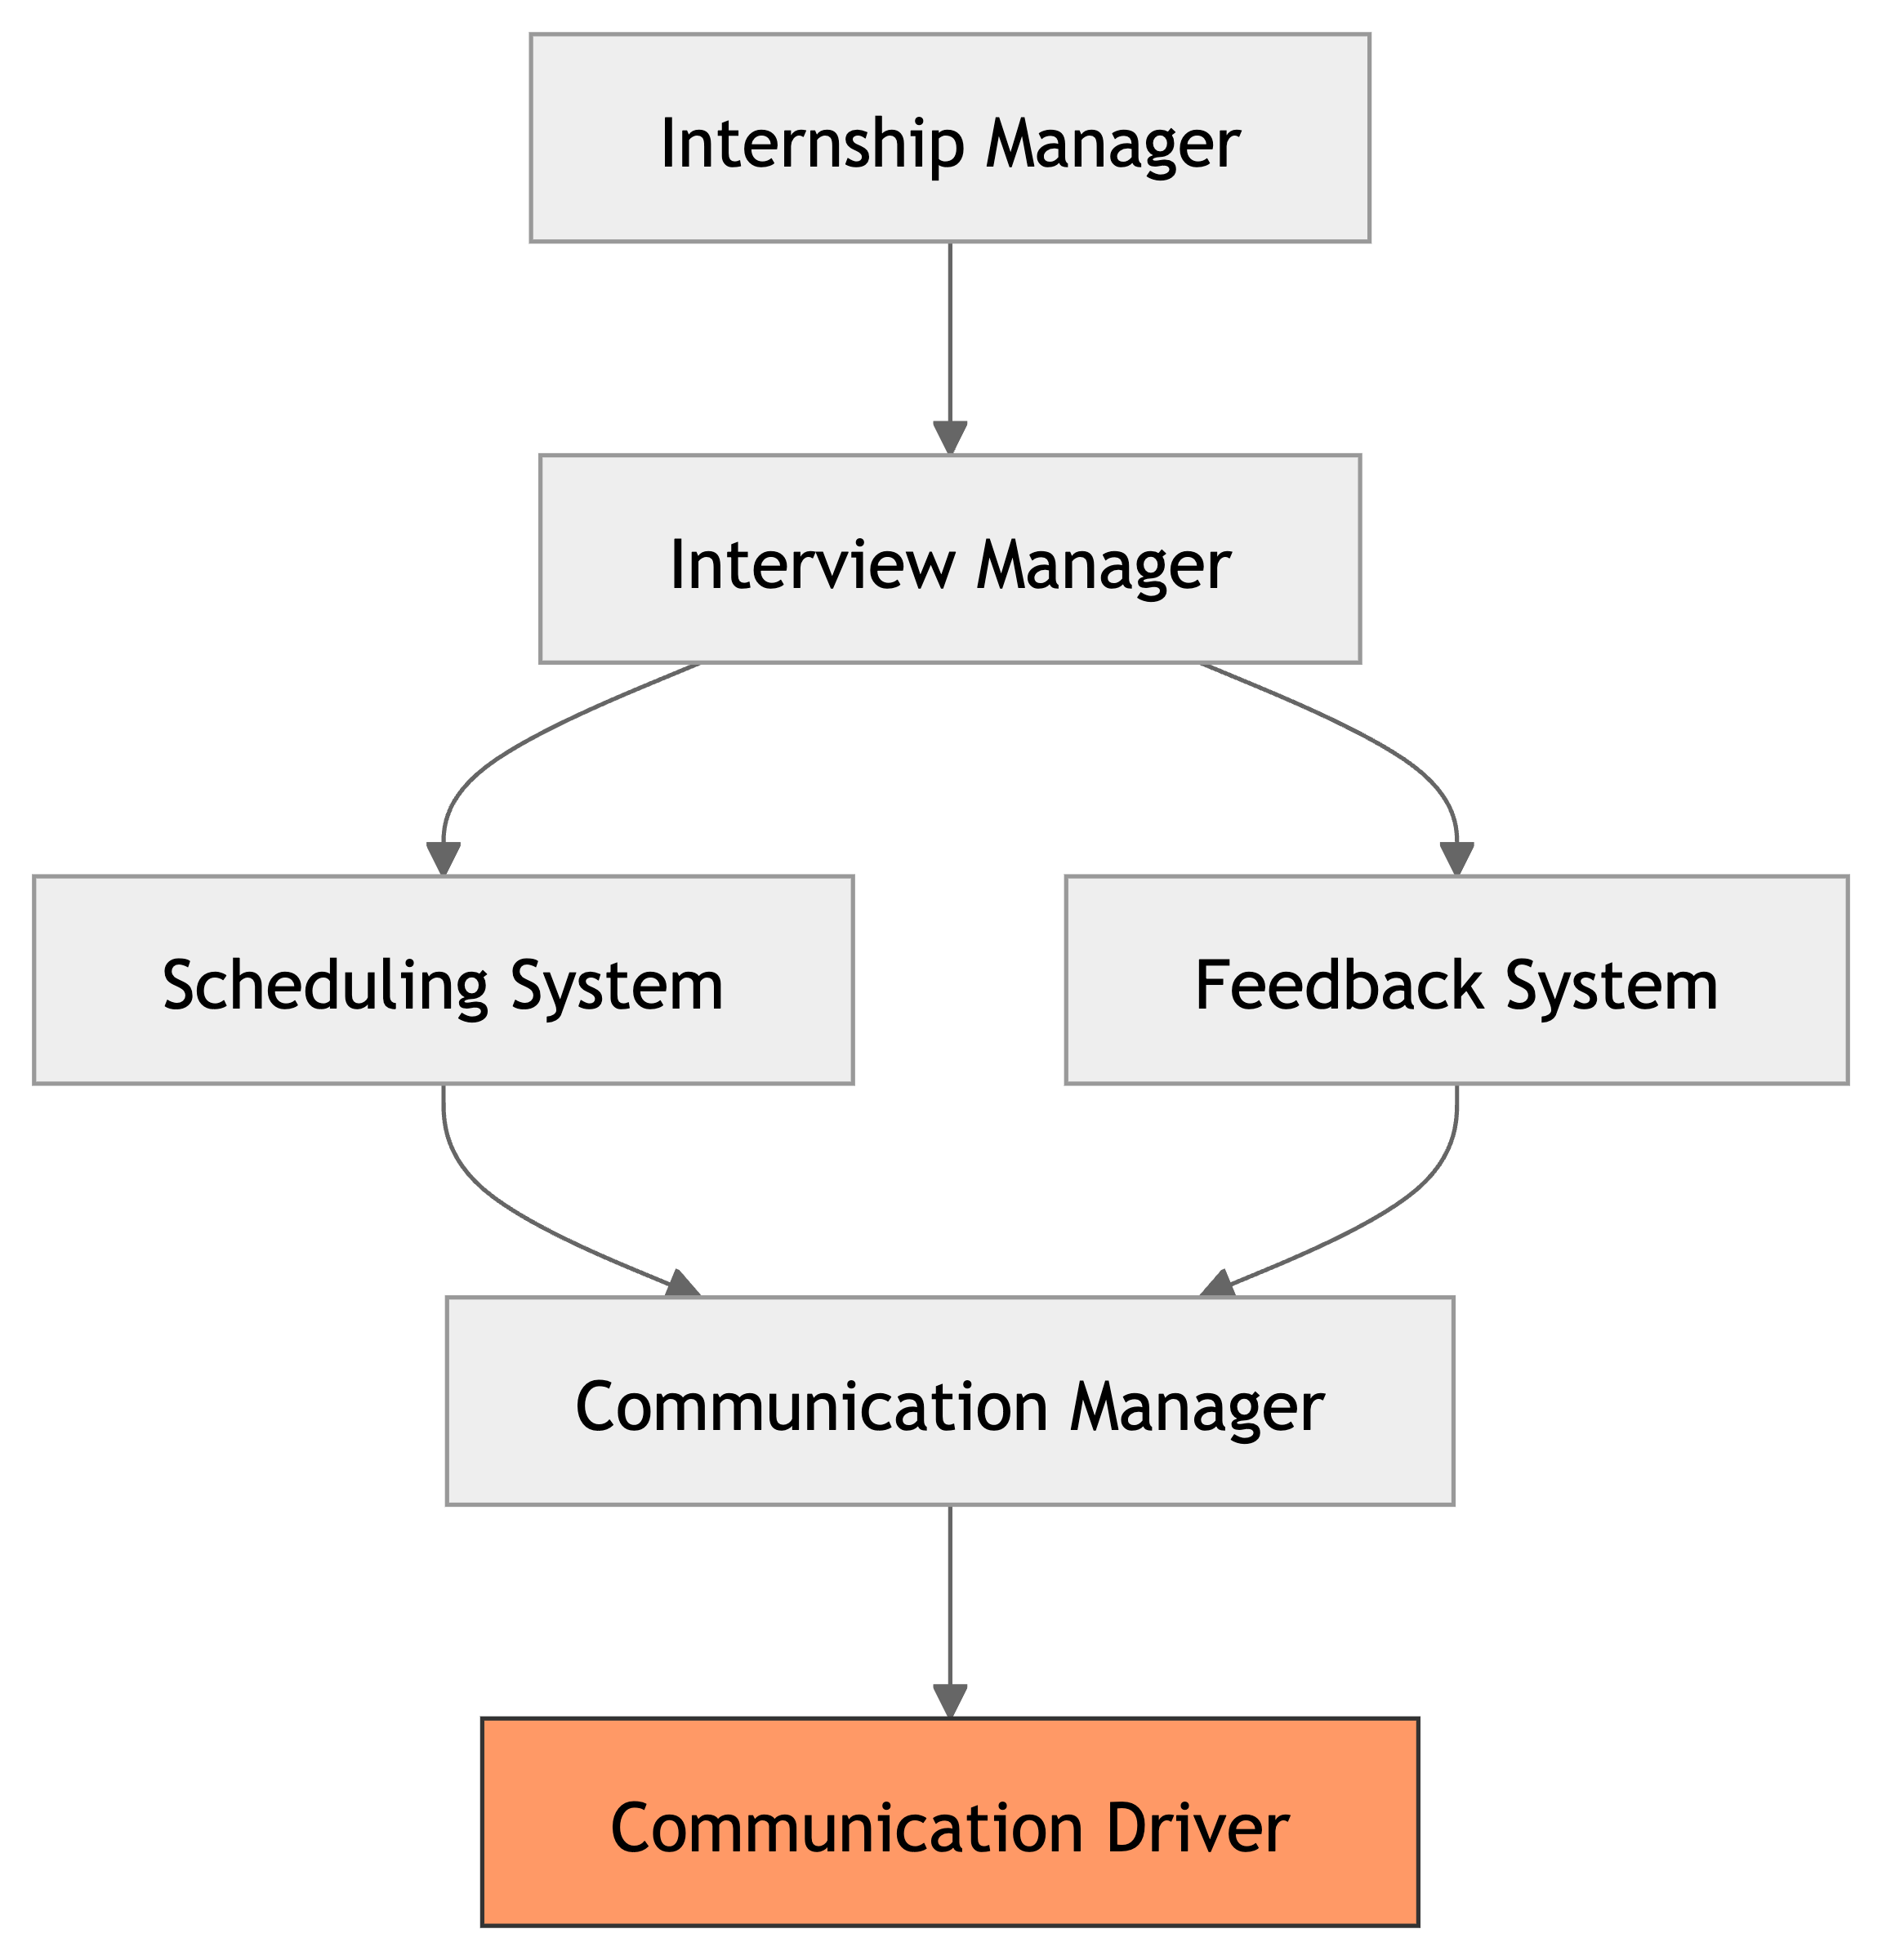
\includegraphics[width=0.59\linewidth]{JhaBhatiaSharma/imagesDD/InterviewandCommunicationIntegration.png}
        \caption{Internship and Communication Integration}
        \label{fig:internshipManagement}
    \end{center}
\end{figure}
The Communication Manager ensures smooth communication and notifications. A \textbf{Communication Driver} will test information flow between the user interface and interview management systems.

\paragraph{Administrative Features Integration}
The \textbf{Admin Manager} is integrated with the following systems:
\begin{itemize}
    \item Monitoring System.
    \item Reporting System.
    \item Complaint System.
\end{itemize}
\begin{figure}[H]
    \begin{center}
      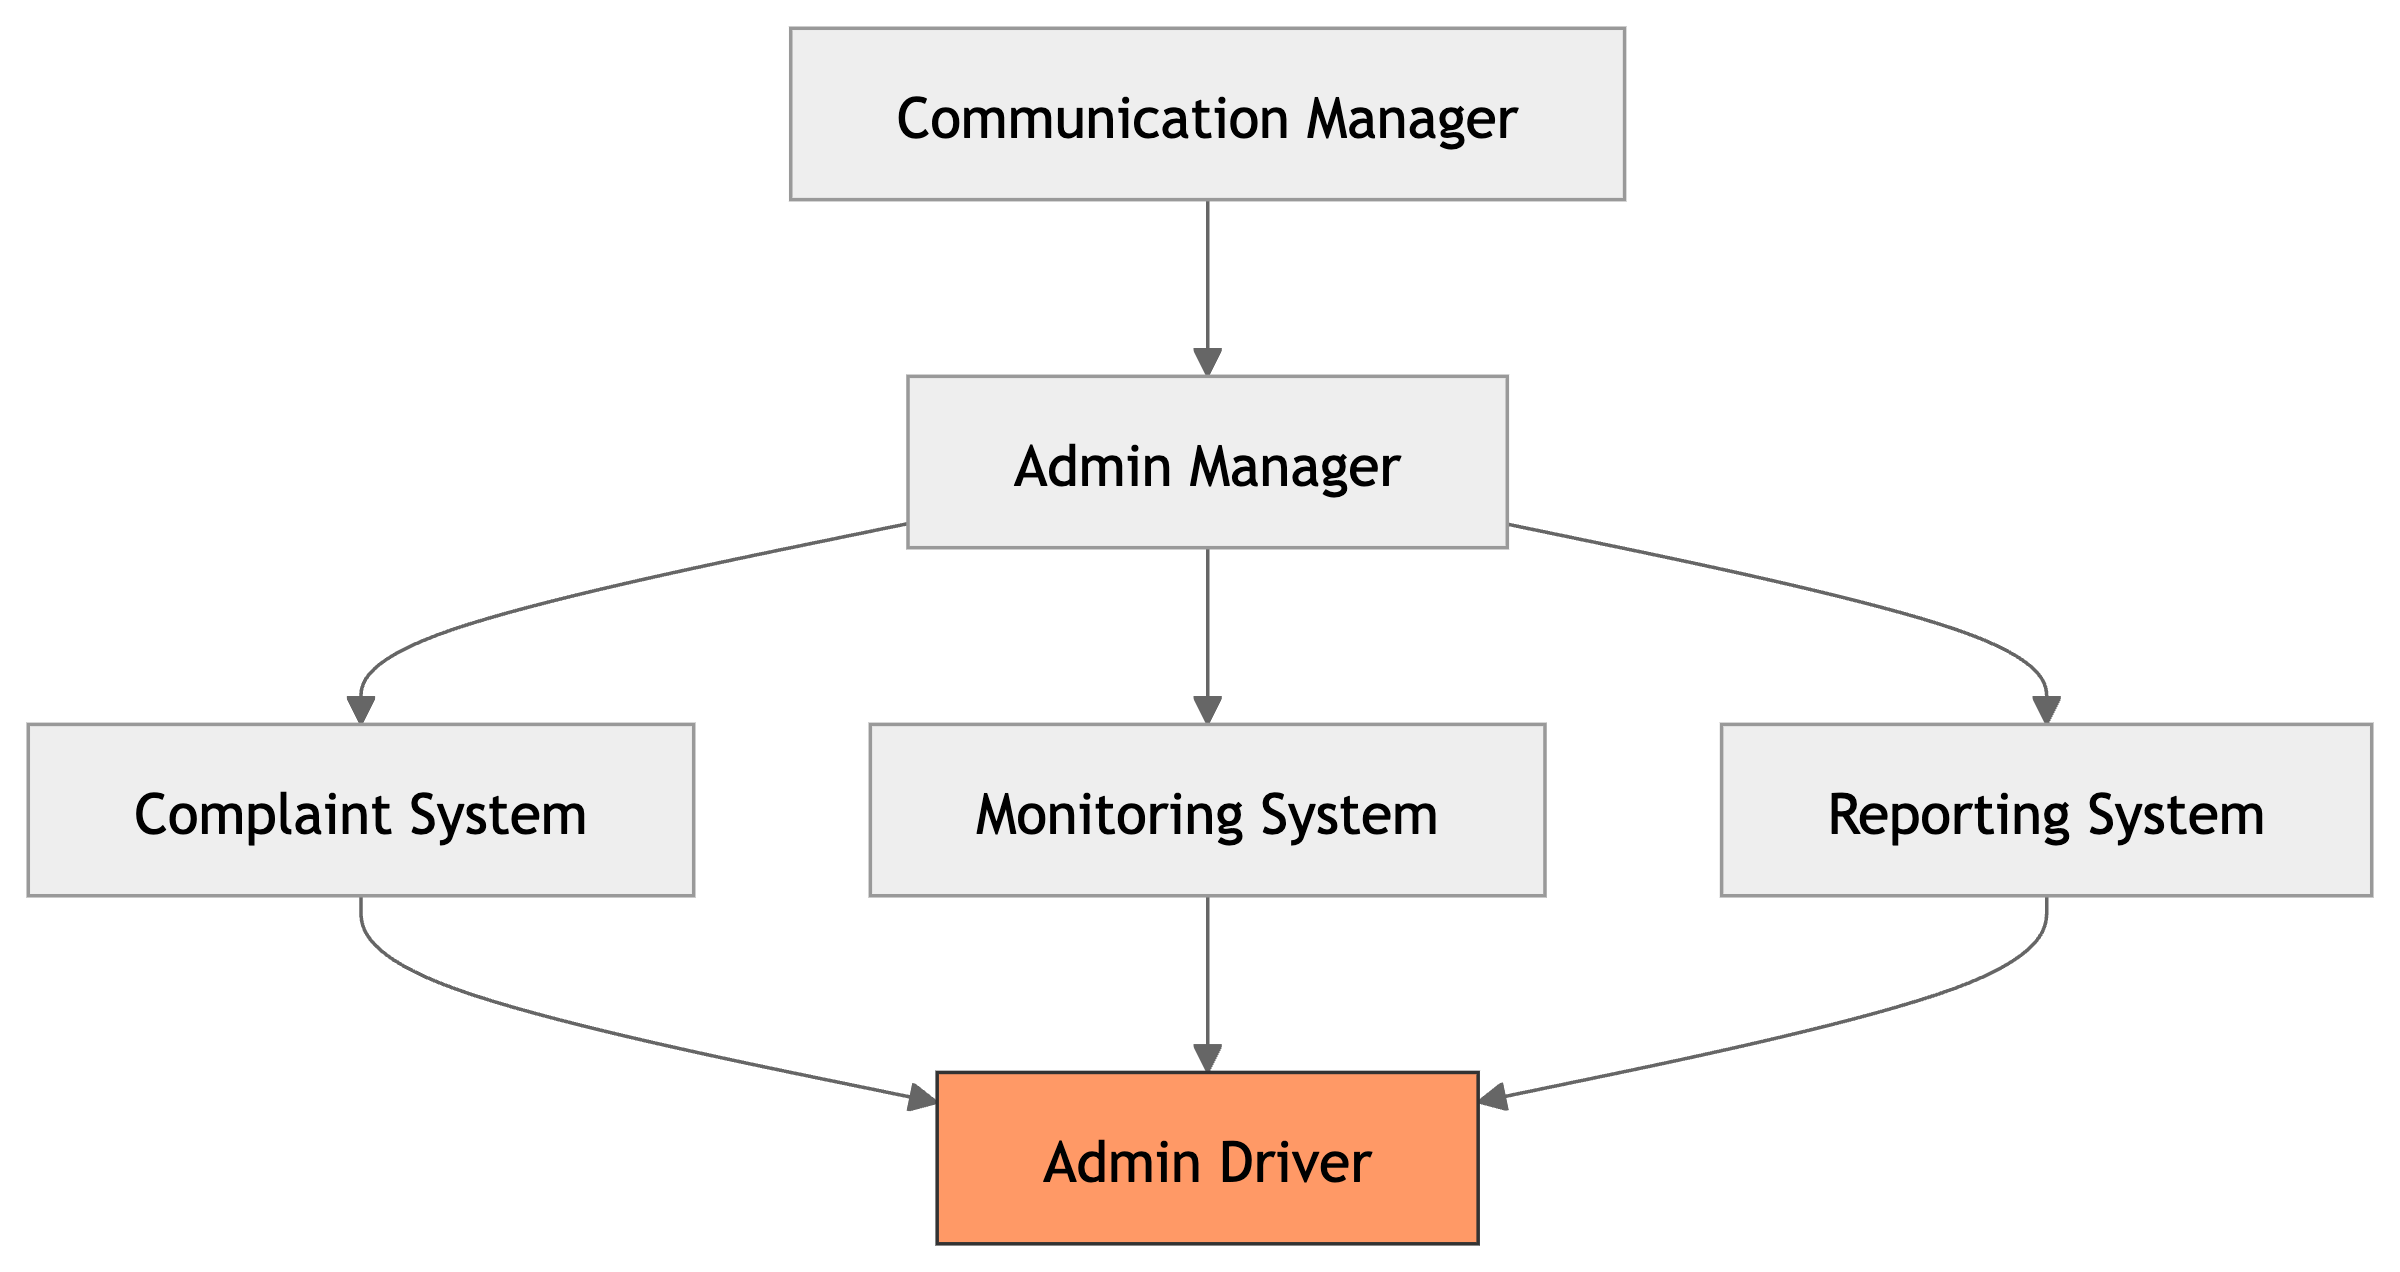
\includegraphics[width=0.59\linewidth]{JhaBhatiaSharma/imagesDD/AdministrativeFeaturesIntegration.png}
        \caption{Administrative Features Integration}
        \label{fig:adminstrativefeatures}
    \end{center}
\end{figure}
This integration includes the Communication Manager to facilitate administrative communication. Functionalities such as complaint management, platform activity monitoring, and report generation will be tested using the \textbf{Admin Driver}. This ensures stability and efficiency in administrative functions.

\paragraph{Final System Integration}
In the final integration phase, all primary managers—Authentication Manager, Profile Manager, Internship Manager, Interview Manager, Communication Manager, and Admin Manager—will be connected to the \textbf{Dashboard Manager}. This integration ensures:
\begin{itemize}
    \item Seamless coordination of data and processes across the platform.
    \item A unified user experience.
\end{itemize}
\begin{figure}[H]
    \begin{center}
      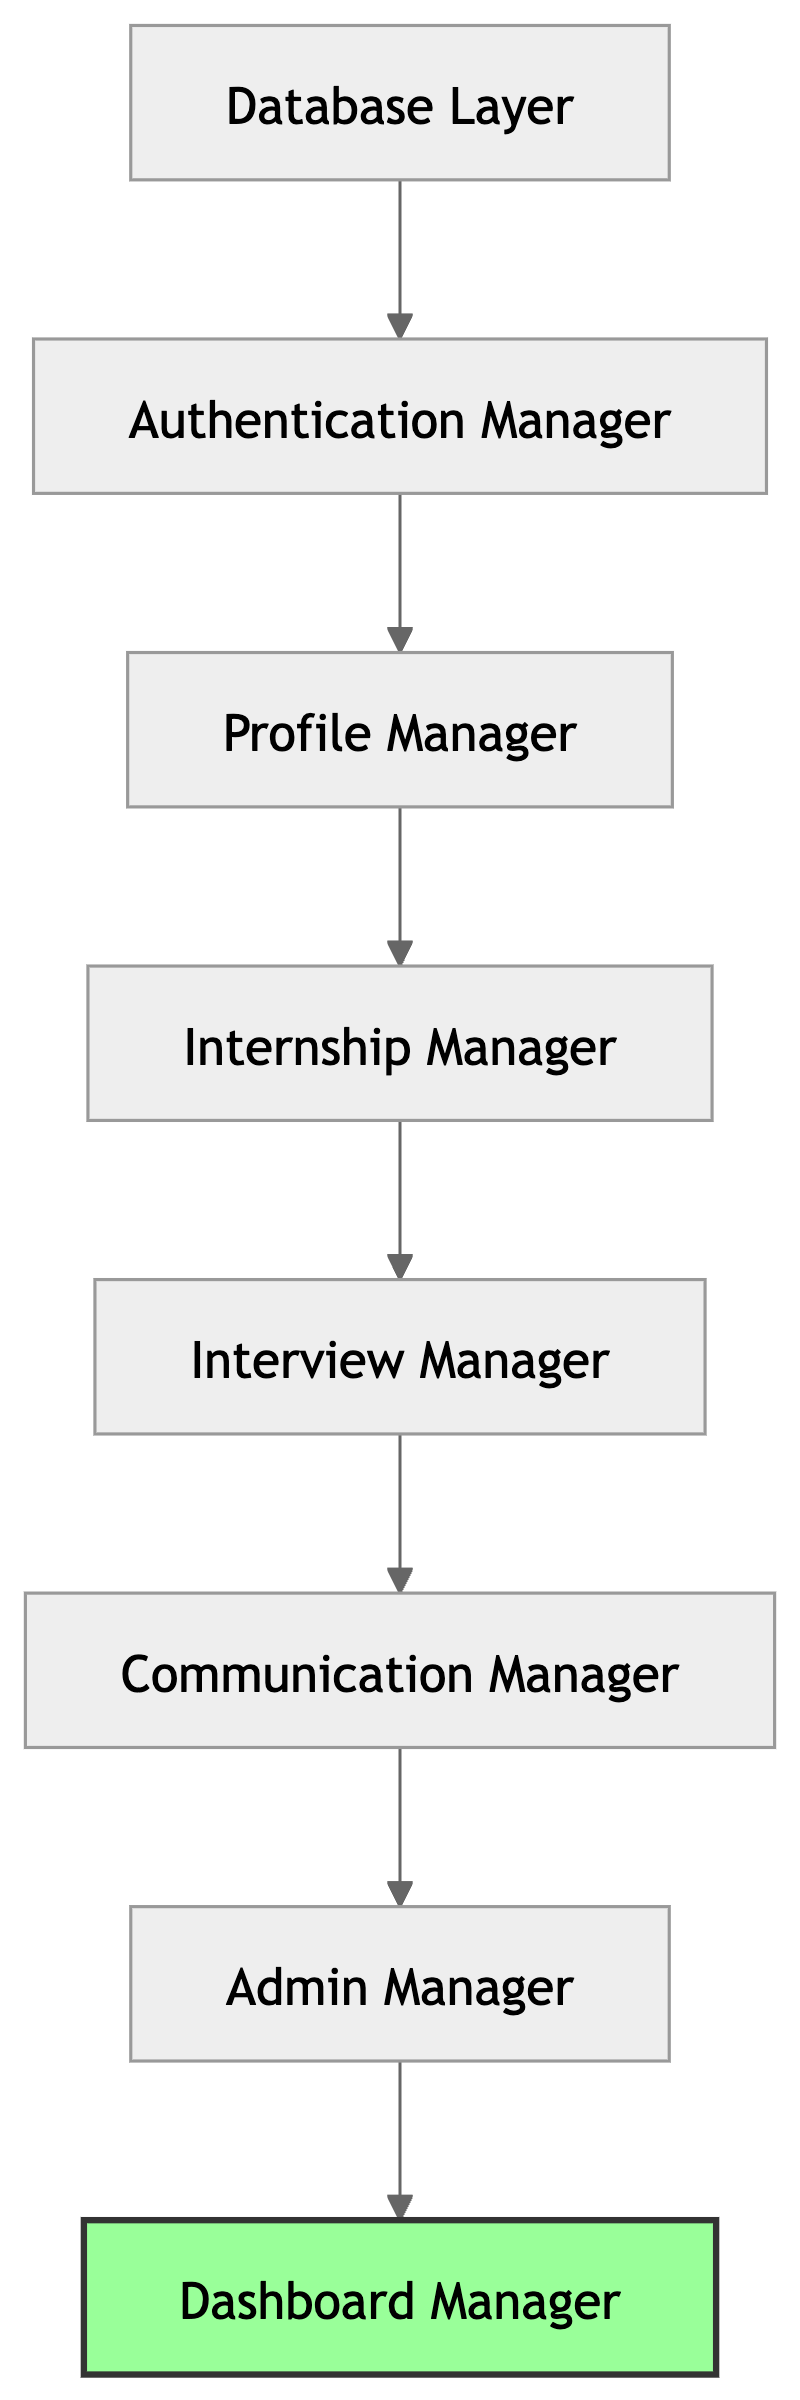
\includegraphics[width=0.18\linewidth]{JhaBhatiaSharma/imagesDD/FinalSystemIntegration.png}
        \caption{Final System Integration}
        \label{fig:finalsystemintegration}
    \end{center}
\end{figure}

The Dashboard Manager acts as the main interface, consolidating data and system processes. This phase marks the completion of the integration process, delivering a fully functional and user-friendly platform.

\section{System Testing Strategy}
\label{sec:system_testing_strategy}

Every newly created component will go through extensive testing before being incorporated into the system to guarantee the platform's accuracy and dependability. To verify each component's unique functionality, drivers will be utilized. After integration, a new driver will test the compatibility of the new component with the existing system, ensuring that module properties are maintained and the overall workflow remains unaffected. Once all components have been integrated, the entire system will undergo testing to confirm its proper operation and ensure the absence of flaws. The following testing methods will be employed:

\subsection{Functional Testing}
Functional testing will confirm that all objectives, specifications, and use cases are satisfied and that the platform complies with the capabilities described in the RASD document. This testing will simulate user scenarios and confirm the system's proper workflow by verifying expected results. Key elements that will be tested include:
\begin{itemize}
    \item Applications
    \item Internship postings
    \item Profile management
    \item Login
    \item Interview scheduling
    \item Complaint handling
\end{itemize}

\subsection{Load Testing}
The system's behavior under various workloads will be evaluated through load testing to identify:
\begin{itemize}
    \item Memory leaks
    \item Buffer overflows
    \item Inefficient memory management
\end{itemize}
This testing ensures that the platform can efficiently manage multiple requests simultaneously and remains stable during periods of high user activity.

\subsection{Performance Testing}
Performance testing will identify bottlenecks and assess how quickly the system responds to demanding workloads. This ensures that:
\begin{itemize}
    \item The platform supports many users concurrently with minimal latency.
    \item Optimization opportunities in the underlying algorithms are identified to improve overall system performance.
\end{itemize}

\subsection{Stress Testing}
Stress testing will simulate extreme scenarios such as:
\begin{itemize}
    \item A large number of users accessing the system simultaneously.
    \item A reduction in processing power.
\end{itemize}
This testing will confirm the platform's robustness and resilience, ensuring minimal user disruption during emergencies or unexpected peak loads.

\subsection{User Interface Testing}
User interface testing will validate the platform's usability and accessibility across a variety of devices and browsers. This testing will:
\begin{itemize}
    \item Ensure a smooth and uniform experience for all user types—students, companies, and administrators.
    \item Verify compatibility with various screen sizes and resolutions.
\end{itemize}

\subsection{Comprehensive Testing Approach}
The system's functionality, reliability, and scalability will be fully verified by combining the following testing techniques:
\begin{itemize}
    \item Functional Testing
    \item Load Testing
    \item Performance Testing
    \item Stress Testing
    \item User Interface Testing
\end{itemize}
This comprehensive approach guarantees:
\begin{itemize}
    \item A flawless user experience.
    \item Compliance with the specifications outlined in the RASD document.
\end{itemize}


    \chapter{Effort Spent}
    \label{ch:effort_spent}%
    \begin{table}[H]
    \centering
    \begin{tabular}{|p{0.25\textwidth}|p{0.5\textwidth}|c|}
        \hline
        \textbf{Team Member} & \textbf{Task} & \textbf{Hours Spent} \\ 
        \hline
        Shreesh Kumar Jha & 
        \begin{enumerate}
            \item Introduction
            \item Architectural Design
            \item User Interface Design
            \item Requirements Traceability
            \item Implementation, Integration, and Test Plan
            \item Effort Spent
            \item References
        \end{enumerate} & 35 \\ 
        \hline
        Samarth Bhatia & 
        \begin{enumerate}
            \item Introduction
            \item Architectural Design
            \item User Interface Design
            \item Requirements Traceability
            \item Implementation, Integration, and Test Plan
            \item Effort Spent
            \item References
        \end{enumerate} & 33 \\ 
        \hline
        Satvik Sharma & 
        \begin{enumerate}
            \item Requirements Analysis
            \item UML Diagrams
            \item Backend Setup
            \item Backend Implementation
            \item API Refactor
        \end{enumerate} & 32 \\ 
        \hline
    \end{tabular}
    \caption{Effort spent by each member of the group.}
    \label{tab:effort_spent}
\end{table}



    \chapter{References}
    \label{ch:references}%
    \section{References}
\label{sec:references}%

\begin{itemize}
    \item Software Engineering 2 Course Materials, A.Y. 2024-2025.
    \item Daniel Jackson, \textit{Software Abstractions: Logic, Language, and Analysis}.
    \item Assignment RDD AY 2024-2025.pdf.
    \item  MongoDB, Inc. (n.d.). \href{https://www.mongodb.com/docs/manual/}{MongoDB Manual}.
    \item Node.js Foundation. (n.d.). \href{https://nodejs.org/en/docs/}{Node.js Documentation.}

\end{itemize}


% LIST OF FIGURES
    \listoffigures

% LIST OF TABLES
    \listoftables
    \cleardoublepage


\end{document}
